% ============================================================
% MediSuivi — Rapport de stage (Overleaf)
% Compiler avec : pdfLaTeX  (Menu > Compiler > pdfLaTeX)
% ============================================================
\documentclass[12pt,a4paper,oneside]{report}

\usepackage[T1]{fontenc}
\usepackage[utf8]{inputenc}
\usepackage[french]{babel}
\usepackage{lmodern}
\usepackage{microtype}
\usepackage[margin=2.5cm]{geometry}
\usepackage{setspace}
\usepackage{graphicx}
\usepackage{float}
\usepackage{xcolor}
\usepackage{array}
\usepackage{booktabs}
\usepackage{longtable}
\usepackage{enumitem}
\usepackage{titlesec}
\usepackage{tocloft}
\usepackage{fancyhdr}
\usepackage{tikz}
\usetikzlibrary{arrows.meta,positioning,shapes.geometric,fit,calc}

% ---------- Styles UML réutilisables (TikZ) ----------
\tikzset{
  uc/.style={draw, thick, ellipse, minimum width=3.6cm, minimum height=1.1cm,
             align=center, fill=teal!10, font=\small},
  seqobj/.style={draw, thick, fill=teal!10, font=\small, align=center,
                 minimum height=0.8cm, minimum width=2.4cm},
  umlbox/.style={draw, thick, align=left, font=\small, fill=white, inner sep=4pt},
  umlsys/.style={draw, thick, dashed, rounded corners},
}
% Acteur UML (bonhomme bâton) : #1=nom de coordinate, #2=position, #3=libellé
\newcommand{\umlactor}[3]{%
  \coordinate (#1) at (#2);
  \draw[thick] (#1) circle (0.16cm);
  \draw[thick] ([yshift=-0.16cm]#1) -- ++(0,-0.5cm);
  \draw[thick] ([yshift=-0.3cm]#1) ++(-0.32cm,0) -- ++(0.64cm,0);
  \draw[thick] ([yshift=-0.66cm]#1) -- ++(-0.26cm,-0.46cm);
  \draw[thick] ([yshift=-0.66cm]#1) -- ++(0.26cm,-0.46cm);
  \node[font=\small, anchor=north] at ([yshift=-1.25cm]#1) {#3};
}
% Classe UML : #1=id node, #2=titre, #3=attributs, #4=opérations
\newcommand{\umlclass}[4]{%
  \node[umlbox] (#1) {%
    \begin{tabular}{l}
      \multicolumn{1}{c}{\textbf{#2}} \\ \hline
      #3 \\ \hline
      #4
    \end{tabular}};
}
\usepackage{hyperref}
\usepackage{bookmark}

\hypersetup{
  colorlinks=true,
  linkcolor=black,
  urlcolor=blue,
  pdftitle={Rapport de stage — MediSuivi},
  pdfauthor={Stage ESPRIT --- Mme Imene Trabelsi}
}

% ---------- Titres en français ----------
\addto\captionsfrench{%
  \renewcommand{\contentsname}{Sommaire}%
  \renewcommand{\listfigurename}{Table des figures}%
  \renewcommand{\listtablename}{Liste des tableaux}%
  \renewcommand{\chaptername}{Chapitre}%
}

% ---------- Style des chapitres ----------
\titleformat{\chapter}[display]
  {\normalfont\huge\bfseries}
  {\chaptertitlename\ \thechapter}
  {14pt}
  {\Huge}
\titlespacing*{\chapter}{0pt}{-20pt}{28pt}

% ---------- Sommaire : points de conduite ----------
\renewcommand{\cftchapdotsep}{\cftdotsep}
\renewcommand{\cftchapleader}{\cftdotfill{\cftchapdotsep}}
\renewcommand{\cftsecleader}{\cftdotfill{\cftdotsep}}
\renewcommand{\cftsubsecleader}{\cftdotfill{\cftdotsep}}
\renewcommand{\cftfigleader}{\cftdotfill{\cftdotsep}}
\renewcommand{\cfttableader}{\cftdotfill{\cftdotsep}}
\setlength{\cftbeforechapskip}{8pt}
\setlength{\cftbeforesecskip}{2pt}
\setcounter{tocdepth}{2}
\setcounter{secnumdepth}{3}

% ---------- En-têtes ----------
\pagestyle{fancy}
\fancyhf{}
\fancyhead[L]{\small\textit{Rapport de stage — MediSuivi}}
\fancyhead[R]{\small\thepage}
\renewcommand{\headrulewidth}{0.4pt}

% ---------- Placeholder de figure ----------
\newcommand{\figplaceholder}[2]{%
  \begin{figure}[htbp]
    \centering
    \fcolorbox{gray!50}{gray!8}{%
      \begin{minipage}{0.88\textwidth}
        \centering
        \vspace{1.8cm}
        {\large\textit{[Insérer la figure]}}\\[0.4em]
        {\small #2}
        \vspace{1.8cm}
      \end{minipage}%
    }
    \caption{#2}
    \label{#1}
  \end{figure}
}

\begin{document}

% ============================================================
% PAGE DE GARDE (à personnaliser)
% ============================================================
\begin{titlepage}
\centering
\vspace*{1.2cm}
{\Large République Tunisienne}\\[0.3em]
{\large Ministère de l'Enseignement Supérieur et de la Recherche Scientifique}\\[1.4cm]
{\Large \textbf{École Supérieure Privée d'Ingénierie et de Technologies}}\\
{\Large \textbf{ESPRIT}}\\[1.6cm]
{\huge\bfseries Rapport de stage}\\[0.6cm]
{\LARGE Conception et réalisation d'une plateforme}\\[0.2cm]
{\LARGE de suivi médical intelligent \textbf{MediSuivi}}\\[1.4cm]
{\large Application web médecin \textbullet\ application mobile patient}\\[0.15cm]
{\large microservices Spring \textbullet\ prédiction IA}\\[2cm]
\begin{tabular}{rl}
\textbf{Réalisé par :} & \textit{À compléter} \\[0.4em]
\textbf{Encadrante :} & Mme Imene Trabelsi \\[0.4em]
\textbf{Organisme d'accueil :} & ESPRIT \\[0.4em]
\textbf{Année universitaire :} & 2025 -- 2026 \\
\end{tabular}
\vfill
\end{titlepage}

\onehalfspacing
\pagenumbering{roman}

\tableofcontents
\clearpage
\listoffigures
\clearpage
\listoftables
\clearpage

\pagenumbering{arabic}

% ============================================================
\chapter*{Introduction générale}
\addcontentsline{toc}{chapter}{Introduction générale}

Le suivi des patients atteints de maladies chroniques (diabète, hypertension, asthme, insuffisance cardiaque) reste fragmenté entre le cabinet médical et le quotidien du patient. \textbf{MediSuivi} vise à relier le médecin et le patient autour d'un même dossier de constantes, de symptômes et d'alertes, enrichi d'une prédiction de gravité.

Ce rapport présente le cadre du stage, la conception globale, puis la réalisation sprint par sprint : authentification, gestion des patients et pathologies, suivi médical, alertes SOS, intelligence artificielle, application mobile, et chaîne DevOps.

% ============================================================
\chapter{Cadre du projet}

Ce premier chapitre situe le stage, réalisé \textbf{au sein d'ESPRIT} sous l'encadrement de \textbf{Mme Imene Trabelsi} : présentation de l'école, organigramme, besoin métier auquel répond \textbf{MediSuivi}, objectifs, démarche Scrum et product backlog.

% ---------- 1.1 ----------
\section{Présentation de l'organisme d'accueil}

Le présent rapport s'inscrit dans le cadre d'un \textbf{stage académique de fin d'études}, effectué à l'\textbf{École Supérieure Privée d'Ingénierie et de Technologies (ESPRIT)}, sous l'encadrement de \textbf{Mme Imene Trabelsi}. L'objet du stage est la conception et la réalisation de la plateforme \textbf{MediSuivi}, destinée au suivi à distance de patients atteints de maladies chroniques.

\subsection{Identité d'ESPRIT}
ESPRIT est un établissement d'enseignement supérieur privé tunisien, créé en 2003 et situé à Charguia~II (Ariana). L'école forme des ingénieurs dans plusieurs filières, notamment l'\textbf{informatique}, le génie civil et le génie électromécanique. Elle appartient au réseau \textbf{Honoris United Universities}. Sa pédagogie combine cours académiques, projets tutorés et mises en situation professionnelles (PFE, stages, ateliers DevOps, développement web et mobile).

Le département d'informatique, au sein duquel ce stage a été réalisé, prépare les étudiants à concevoir des systèmes d'information distribués : applications web et mobiles, architectures microservices, qualité logicielle et intégration continue. MediSuivi s'inscrit directement dans cette orientation.

\subsection{Encadrement}
L'encadrement pédagogique et technique a été assuré par \textbf{Mme Imene Trabelsi}, enseignante à ESPRIT. Son rôle a couvert :
\begin{itemize}[leftmargin=1.4em]
  \item la validation du périmètre et du product backlog ;
  \item le suivi des sprints (revues, priorisation, retours sur la conception UML et le code) ;
  \item l'exigence de qualité (tests, SonarQube, industrialisation Jenkins / Docker).
\end{itemize}
Il n'y a pas d'organisme industriel distinct : l'école est à la fois \textbf{établissement de formation} et \textbf{organisme d'accueil} du stage.

\subsection{Intérêt du projet pour ESPRIT}
Pour l'école, MediSuivi constitue un \textbf{projet intégrateur} : il articule le métier (télésuivi médecin--patient) et la stack enseignée (Spring Cloud, React, React Native, FastAPI, Jenkins, SonarQube, Docker). Il peut servir de démonstrateur pédagogique (architecture microservices, client web et mobile, module d'intelligence artificielle).

\subsection{Missions confiées au stagiaire}
Les missions confiées par Mme Trabelsi correspondent au périmètre livré :
\begin{itemize}[leftmargin=1.4em]
  \item concevoir l'architecture microservices (Config Server, Eureka, Gateway, \texttt{user-service}, \texttt{patient-service}) ;
  \item réaliser le portail médecin (\texttt{medsuivifront}) ;
  \item réaliser l'application patient Expo / React Native (\texttt{medsuivi\_patient\_mobile}) ;
  \item exposer un service de prédiction de gravité (\texttt{medisuivi\_predict\_api}) ;
  \item industrialiser les builds (Jenkins, tests, SonarQube, images Docker).
\end{itemize}

% ---------- 1.2 ----------
\section{Organigramme de l'organisme}

La figure~\ref{fig:organigramme} situe le projet MediSuivi dans l'organisation d'ESPRIT : le stage relève du \textbf{département Informatique}, sous l'encadrement de \textbf{Mme Imene Trabelsi}.

\begin{figure}[htbp]
\centering
\begin{tikzpicture}[
  font=\small,
  box/.style={draw, rounded corners=2pt, align=center, inner sep=6pt, minimum width=3.35cm, minimum height=1.05cm},
  dg/.style={box, fill=teal!18, font=\bfseries\small, minimum width=4.2cm},
  dir/.style={box, fill=blue!12},
  eq/.style={box, fill=orange!15, minimum width=3.2cm},
  arr/.style={-{Latex}, thick}
]
\node[dg] (dg) {Direction générale\\ESPRIT};
\node[dir, below left=1.2cm and 0.35cm of dg] (etudes) {Direction\\des études};
\node[dir, below=1.2cm of dg] (info) {Département\\Informatique};
\node[dir, below right=1.2cm and 0.35cm of dg] (pfe) {Pôle PFE /\\stages};
\node[eq, below=1.1cm of info] (enc) {\textbf{Mme Imene Trabelsi}\\Encadrante};
\node[eq, below=1.05cm of enc] (proj) {\textbf{Projet MediSuivi}\\Stagiaire};
\draw[arr] (dg) -- (etudes);
\draw[arr] (dg) -- (info);
\draw[arr] (dg) -- (pfe);
\draw[arr] (info) -- (enc);
\draw[arr] (enc) -- (proj);
\draw[arr] (pfe.south) -- ++(0,-0.35) -| (enc.east);
\end{tikzpicture}
\caption{Organigramme d'ESPRIT et positionnement du stage MediSuivi}
\label{fig:organigramme}
\end{figure}

Le stagiaire est rattaché au département Informatique. Les échanges avec Mme Trabelsi portent sur le backlog, les revues de sprint et la validation des incréments (web, mobile, API, DevOps).

% ---------- 1.3 ----------
\section{Contexte et problématique}

Les maladies chroniques (diabète, hypertension artérielle, asthme, insuffisance cardiaque) exigent un suivi régulier des constantes et des symptômes, souvent en dehors du cabinet. Dans la pratique actuelle, ce suivi reste \textbf{fragmenté} : le patient note ses valeurs sur papier ou dans une application grand public, tandis que le médecin ne les voit qu'au prochain rendez-vous. Une aggravation (pic de glycémie, dyspnée, alerte vitale) peut donc passer inaperçue.

Plusieurs limites concrètes motivent MediSuivi :
\begin{itemize}[leftmargin=1.4em]
  \item \textbf{Absence de fil continu} entre le domicile et le dossier médecin ;
  \item \textbf{Pas de canal d'urgence simple} : le patient n'a pas toujours un moyen immédiat de signaler une situation critique à \emph{son} médecin ;
  \item \textbf{Lecture tardive du risque} : le niveau de gravité est souvent estimé trop tard, sans s'appuyer sur la tendance des mesures (moyenne, dispersion, pente sur plusieurs jours) ni sur les symptômes récents ;
  \item \textbf{Outils cloisonnés} : un portail métier pour le soignant et une application mobile pour le patient sont rarement conçus comme un même système.
\end{itemize}

La problématique peut se formuler ainsi : \emph{comment concevoir une plateforme unique, sûre et évolutive, qui permette au patient de saisir ses constantes et d'alerter, et au médecin de suivre, prioriser et anticiper le risque, y compris à l'aide d'un modèle prédictif ?}

MediSuivi y répond par quatre piliers : un \textbf{portail web médecin}, une \textbf{application mobile patient}, un \textbf{backend microservices} (comptes, patients, mesures, symptômes, alertes) et une \textbf{API de prédiction de gravité} (Random Forest, FastAPI), le tout industrialisé (tests, SonarQube, Jenkins, Docker).

% ---------- 1.4 ----------
\section{Objectifs du projet MediSuivi}

L'objectif général est de réaliser une plateforme de \textbf{suivi médical intelligent} reliant médecin et patient autour d'un même dossier.

\paragraph{Objectifs fonctionnels.}
\begin{itemize}[leftmargin=1.4em]
  \item Authentifier les utilisateurs (médecin et patient), gérer l'inscription, le mot de passe oublié, le profil et la photo.
  \item Permettre au médecin de gérer ses patients, le catalogue de pathologies et l'affectation d'une maladie à un patient.
  \item Enregistrer des constantes (tension, glycémie, fréquence cardiaque, température, poids, SpO$_2$) et des symptômes, puis les consulter sous forme d'historique et de courbe.
  \item Offrir une alerte SOS côté patient et un centre d'alertes côté médecin (consultation et traitement).
  \item Proposer une prédiction de gravité à partir des caractéristiques cliniques et de la tendance des relevés.
\end{itemize}

\paragraph{Objectifs techniques.}
\begin{itemize}[leftmargin=1.4em]
  \item Découper le backend en microservices Spring Cloud (configuration centralisée, découverte Eureka, API Gateway).
  \item Séparer le métier « comptes » (\texttt{user-service}) du métier « dossier médical » (\texttt{patient-service}).
  \item Exposer le modèle d'IA via un service Python indépendant, appelé par le \texttt{patient-service}.
  \item Couvrir le code par des tests (JUnit, Vitest, pytest) et une analyse SonarQube.
  \item Automatiser l'intégration continue et la publication d'images Docker.
\end{itemize}

\paragraph{Objectifs pédagogiques.}
Le stage vise à mettre en pratique le cycle de vie d'un produit logiciel (analyse, conception UML, implémentation, tests, déploiement) et le travail en sprints Scrum.

% ---------- 1.5 ----------
\section{Méthodologie Scrum}

Face à un périmètre large (deux clients, plusieurs services, un module IA, une chaîne DevOps), une démarche \textbf{prédictive} (cycle en V intégral avant tout code) aurait figé trop tôt les choix. La méthode \textbf{Scrum} a été retenue : le besoin est découpé en \emph{user stories}, livrées par sprints, avec un incrément démontrable à chaque revue.

Les rôles Scrum ont été adaptés au contexte d'un stage académique à ESPRIT :
\begin{itemize}[leftmargin=1.4em]
  \item \textbf{Product Owner} : \textbf{Mme Imene Trabelsi} (priorisation du backlog, validation métier et pédagogique) ;
  \item \textbf{Scrum Master} : animation des cérémonies et levée des obstacles (rôle partagé avec le stagiaire) ;
  \item \textbf{Équipe de développement} : le stagiaire, responsable de la conception et de la réalisation des incréments.
\end{itemize}

Les artefacts utilisés sont le \textbf{product backlog} (section~\ref{sec:backlog}), le \textbf{sprint backlog} et l'\textbf{incrément} (portail, application, API). Les cérémonies suivies sont la planification, le daily (point court), la revue et la rétrospective. Chaque sprint vise un thème cohérent (authentification, patients, suivi, alertes, IA, mobile) afin de limiter le travail en cours et de pouvoir démontrer une fonctionnalité de bout en bout.

% ---------- 1.6 ----------
\section{Cycle de vie Scrum}

Le cycle Scrum est itératif : à partir du product backlog, un sprint backlog est constitué ; pendant le sprint, l'équipe développe, teste et intègre ; la revue inspecte l'incrément ; la rétrospective améliore le processus ; le backlog est ensuite réordonné.

\begin{figure}[htbp]
\centering
\begin{tikzpicture}[
  font=\small,
  node distance=0.55cm and 0.7cm,
  phase/.style={draw, rounded corners=3pt, align=center, inner sep=7pt, minimum width=2.55cm, minimum height=1.15cm, fill=teal!12},
  art/.style={draw, rounded corners=2pt, align=center, inner sep=5pt, fill=orange!12, minimum width=2.35cm},
  arr/.style={-{Latex}, thick}
]
\node[phase] (pb) {Product\\backlog};
\node[phase, right=of pb] (plan) {Sprint\\planning};
\node[phase, right=of plan] (spr) {Sprint\\(dev + tests)};
\node[phase, below=1.35cm of spr] (rev) {Sprint\\review};
\node[phase, left=of rev] (ret) {Rétro-\\spective};
\node[art, below=1.35cm of pb] (inc) {Incrément\\livrable};
\draw[arr] (pb) -- (plan);
\draw[arr] (plan) -- (spr);
\draw[arr] (spr) -- (rev);
\draw[arr] (rev) -- (ret);
\draw[arr] (ret.west) -- ++(-0.85,0) |- (pb.west);
\draw[arr] (spr) -- (inc);
\node[art, above=0.55cm of spr] (sb) {Sprint backlog};
\draw[arr] (plan) |- (sb);
\end{tikzpicture}
\caption{Cycle de vie Scrum appliqué au projet MediSuivi}
\label{fig:scrum}
\end{figure}

Dans MediSuivi, un sprint se termine typiquement par : des API stables derrière la Gateway, un écran web et/ou mobile utilisable, et des tests automatisés. Le sprint suivant s'appuie sur cet incrément (par exemple : sans authentification JWT, pas de dossier patient ; sans mesures, pas de prédiction de gravité).

% ---------- 1.7 ----------
\section{Product Backlog}
\label{sec:backlog}

Le product backlog rassemble les besoins, exprimés en \emph{user stories}, classés par épic et par priorité. Il a servi de contrat de périmètre tout au long du stage. Le tableau~\ref{tab:backlog} en donne une vue macro ; le tableau~\ref{tab:stories} détaille les stories réalisées.

\begin{table}[htbp]
\centering
\begin{tabular}{@{}clp{7.6cm}c@{}}
\toprule
\textbf{ID} & \textbf{Épic} & \textbf{Description} & \textbf{Priorité} \\
\midrule
E1 & Authentification & Inscription, connexion JWT, mot de passe oublié, profil & Haute \\
E2 & Patients        & CRUD patients, filtre par niveau de risque, profil médecin & Haute \\
E3 & Pathologies     & Catalogue de maladies et affectation à un patient & Haute \\
E4 & Suivi           & Mesures, symptômes, historique, courbes d'évolution & Haute \\
E5 & Alertes         & SOS patient, centre d'alertes médecin, traitement & Haute \\
E6 & Prédiction IA   & Features, Random Forest, FastAPI, scoring médecin & Moyenne \\
E7 & Application mobile & Accueil, saisie, SOS, historique, profil patient & Haute \\
E8 & Qualité / DevOps & Tests, SonarQube, Jenkins, Docker Hub & Moyenne \\
\bottomrule
\end{tabular}
\caption{Product backlog MediSuivi --- vue par épics}
\label{tab:backlog}
\end{table}

\begin{table}[htbp]
\centering
\small
\begin{tabular}{@{}clp{8.4cm}c@{}}
\toprule
\textbf{ID} & \textbf{En tant que} & \textbf{Je veux} & \textbf{Sprint} \\
\midrule
US01 & Médecin  & m'inscrire et me connecter au portail & 1 \\
US02 & Utilisateur & réinitialiser mon mot de passe par e-mail & 1 \\
US03 & Utilisateur & mettre à jour mon profil et ma photo & 1 \\
US04 & Patient & me connecter à l'application mobile & 1 / 6 \\
US05 & Médecin  & consulter une vue d'ensemble de mon activité & 2 \\
US06 & Médecin  & créer, rechercher et filtrer mes patients & 2 \\
US07 & Médecin  & gérer le catalogue de pathologies & 2 \\
US08 & Médecin  & affecter une maladie à un patient & 2 \\
US09 & Médecin / Patient & saisir une constante (tension, glycémie, \ldots) & 3 \\
US10 & Médecin  & consigner un symptôme et sa gravité & 3 \\
US11 & Patient & consulter l'historique et la courbe d'évolution & 3 / 6 \\
US12 & Patient & envoyer une alerte SOS à mon médecin & 4 \\
US13 & Médecin  & consulter et traiter les alertes & 4 \\
US14 & Médecin  & lancer une prédiction de gravité (IA) & 5 \\
US15 & Système  & publier les services via Jenkins et Docker & 5 / DevOps \\
\bottomrule
\end{tabular}
\caption{Extrait du product backlog --- user stories}
\label{tab:stories}
\end{table}

Ces stories seront détaillées, sprint par sprint, dans les chapitres de réalisation (diagrammes de cas d'utilisation, de séquence et de classes, puis interfaces). Le chapitre suivant présente l'analyse globale et l'architecture retenue pour satisfaire ce backlog.

% ============================================================
\chapter{Analyse et conception globale}

\section{Étude de l'existant}
\textit{Décrire les solutions existantes de télésuivi et leurs limites.}

\section{Identification des acteurs}
Deux acteurs principaux : le \textbf{médecin} (portail web) et le \textbf{patient} (application mobile). Les services techniques (Gateway, User Service, Patient Service, Predict API) sont des acteurs secondaires.

\section{Diagramme de cas d'utilisation global}
\figplaceholder{fig:uc-global}{Diagramme de cas d'utilisation global}

\section{Planification des sprints}
\figplaceholder{fig:sprints}{Planification des sprints}

\begin{table}[htbp]
\centering
\begin{tabular}{@{}clp{8.6cm}@{}}
\toprule
\textbf{Sprint} & \textbf{Thème} & \textbf{Livrable} \\
\midrule
1 & Authentification & Login, register, reset password, JWT, profil \\
2 & Patients \& pathologies & Dashboard, CRUD patients, maladies \\
3 & Suivi médical & Mesures, symptômes, historique, courbes \\
4 & Alertes & SOS mobile, centre d'alertes, traitement \\
5 & Prédiction IA & FastAPI, Random Forest, scoring médecin \\
6 & Application mobile & Accueil, saisie, SOS, historique, profil \\
\bottomrule
\end{tabular}
\caption{Planification des sprints MediSuivi}
\label{tab:sprints}
\end{table}

\section{Choix technologiques}
\begin{table}[htbp]
\centering
\begin{tabular}{@{}llp{6.8cm}@{}}
\toprule
\textbf{Couche} & \textbf{Technologie} & \textbf{Dépôt} \\
\midrule
Portail médecin & React, TypeScript, Vite & \texttt{medsuivifront} \\
App patient & React Native, Expo & \texttt{medsuivi\_patient\_mobile} \\
Backend & Spring Boot / Cloud & \texttt{medsuivistage} \\
IA & FastAPI, scikit-learn & \texttt{medisuivi\_predict\_api} \\
CI/CD & Jenkins, SonarQube, Docker & Jenkinsfiles des dépôts \\
\bottomrule
\end{tabular}
\caption{Stack technique du projet}
\label{tab:stack}
\end{table}

\section{Architecture physique}
\figplaceholder{fig:arch-phys}{Architecture physique}

\section{Architecture logique}
\figplaceholder{fig:arch-log}{Architecture logique}

\section{Architecture microservices du projet}
\figplaceholder{fig:arch-micro}{Architecture microservices de MediSuivi}

\subsection{Config Server}
Centralisation des fichiers de configuration des services Spring Cloud.

\subsection{Discovery (Eureka)}
Enregistrement et découverte des instances (\texttt{discovery}).

\subsection{API Gateway}
Point d'entrée unique, routage vers \texttt{user-service} et \texttt{patient-service}.

\subsection{User Service}
Comptes, authentification JWT, inscription, mot de passe oublié, gestion des utilisateurs.

\subsection{Patient Service}
Médecins, patients, maladies, mesures, symptômes, alertes, appel de prédiction.

\subsection{Predict API (Python / FastAPI)}
\figplaceholder{fig:arch-python}{Architecture du Predict API (Python)}

\section{Architecture des clients (web médecin et mobile patient)}

Cette section présente l'architecture des deux interfaces clientes de la plateforme
\textit{MediSuivi} : l'application web destinée aux médecins et l'application mobile
dédiée aux patients. Toutes deux consomment exclusivement l'API Gateway et partagent
le même mécanisme d'authentification par jeton JWT.

% ─────────────────────────────────────────────────────────────
\subsection{Application mobile patient (React Native / Expo)}
% ─────────────────────────────────────────────────────────────

L'application mobile patient est développée avec \textbf{React Native} (v0.86) et le
framework \textbf{Expo} (v57), ce qui lui permet d'être déployée aussi bien sur
Android que sur iOS à partir d'une base de code unique.

\subsubsection{Structure en couches}

L'architecture de l'application mobile suit un découpage en couches bien délimitées :

\begin{itemize}
  \item \textbf{Couche de navigation} : fondée sur \texttt{@react-navigation},
    elle orchestre deux niveaux de navigation. Un
    \texttt{AppNavigator} (pile native) redirige le flux selon l'état
    d'authentification : vers l'écran de connexion si l'utilisateur n'est
    pas authentifié, ou vers le \texttt{MainTabNavigator} (onglets inférieurs)
    dans le cas contraire. Ce dernier expose cinq onglets :
    \textit{Accueil}, \textit{Saisie}, \textit{Alerte SOS}, \textit{Historique}
    et \textit{Profil}.

  \item \textbf{Couche de présentation (Screens)} : cinq écrans constituent
    l'interface principale de l'application :
    \begin{itemize}
      \item \texttt{DashboardScreen} -- tableau de bord affichant les indicateurs
        de santé du patient et les graphiques d'évolution ;
      \item \texttt{AddMeasureScreen} -- formulaire de saisie d'une nouvelle
        mesure clinique (glycémie, tension, etc.) ;
      \item \texttt{SendAlertScreen} -- déclenchement d'une alerte médicale
        d'urgence (SOS) ;
      \item \texttt{HistoryScreen} -- historique des relevés
        enregistrés ;
      \item \texttt{ProfileScreen} -- consultation et modification du profil
        patient.
    \end{itemize}

  \item \textbf{Couche des composants réutilisables} : des composants génériques
    (\texttt{Button}, \texttt{Card}, \texttt{InputField}, \texttt{MeasureCard},
    \texttt{RiskBadge}, \texttt{EvolutionChart}) encapsulent la logique
    d'affichage et garantissent la cohérence visuelle de l'interface.

  \item \textbf{Couche de gestion d'état (Context API)} : un
    \texttt{AuthContext} expose à toute l'application l'état de session
    (\texttt{user}, \texttt{patient}, \texttt{token}) ainsi que les actions
    \texttt{login}, \texttt{logout} et \texttt{refreshPatient}. L'état est
    initialisé depuis le stockage local (\texttt{AsyncStorage}) au démarrage
    de l'application.

  \item \textbf{Couche de services (API)} : un client HTTP \textbf{Axios}
    centralisé dans \texttt{api.ts} est configuré avec :
    \begin{itemize}
      \item un \textit{intercepteur de requête} qui injecte automatiquement
        le jeton JWT (\texttt{Bearer}) dans chaque appel et résout dynamiquement
        l'URL de base (configurable via \texttt{AsyncStorage}) ;
      \item un \textit{intercepteur de réponse} qui intercepte les erreurs
        \texttt{HTTP 401} et déclenche une déconnexion automatique.
    \end{itemize}
    Les services métier (\texttt{authService}, \texttt{patientService},
    \texttt{suiviService}) consomment ce client pour communiquer avec
    l'API Gateway du back-end.
\end{itemize}

\subsubsection{Authentification et sécurité}

L'authentification s'appuie sur un mécanisme JWT. Lors de la connexion,
le service \texttt{authService} envoie les identifiants au point d'entrée
\texttt{/auth/login} de l'API Gateway, récupère le jeton et le persiste dans
\texttt{AsyncStorage}. Un contrôle de rôle côté client garantit que seuls les
comptes de type \texttt{PATIENT} peuvent accéder à l'application mobile ; tout
autre rôle (médecin, administrateur) se voit refuser l'accès. À chaque démarrage,
le profil patient est rafraîchi depuis le serveur afin d'afficher les données
les plus récentes, notamment le niveau de risque calculé par le micro-service
d'analyse.

% ─────────────────────────────────────────────────────────────
\subsection{Présentation des interfaces de l'application mobile patient}
% ─────────────────────────────────────────────────────────────

L'application mobile \textit{MediSuivi} propose cinq écrans principaux,
accessibles via une barre de navigation inférieure, précédés d'un écran de
connexion. Les figures suivantes illustrent chacune de ces interfaces.

% ─── Figure : Connexion ───────────────────────────────────────────────
\begin{figure}[H]
  \centering
  
\includegraphics[width=0.45\textwidth]{login.png}
  \caption{Écran de connexion --- Authentification du patient}
  \label{fig:mobile-login}
\end{figure}

L'écran de connexion (Figure~\ref{fig:mobile-login}) présente une interface
épurée sur fond beige chaud (\texttt{\#F3EFE6}). Le patient saisit son
identifiant ou adresse email et son mot de passe. Un contrôle de rôle est
effectué côté client : seuls les comptes de type \texttt{PATIENT} sont admis.

% ─── Figure : Tableau de bord ─────────────────────────────────────────
\begin{figure}[H]
  \centering
  
\includegraphics[width=0.45\textwidth]{dashboard.png}
  \caption{Tableau de bord patient --- Vue générale de l'état de santé}
  \label{fig:mobile-dashboard}
\end{figure}

Le tableau de bord (Figure~\ref{fig:mobile-dashboard}) constitue la page
d'accueil principale. Il affiche le niveau de risque calculé par le
micro-service d'analyse (\textit{RISQUE FAIBLE / MODÉRÉ / ÉLEVÉ / CRITIQUE}),
les informations du médecin référent, les trois dernières mesures enregistrées,
ainsi que des boutons d'action rapide pour saisir une mesure ou déclencher
une alerte.

% ─── Figure : Saisie de mesure ────────────────────────────────────────
\begin{figure}[H]
  \centering
  
\includegraphics[width=0.45\textwidth]{add_measure.png}
  \caption{Écran de saisie --- Enregistrement d'une nouvelle constante médicale}
  \label{fig:mobile-addmeasure}
\end{figure}

L'écran de saisie (Figure~\ref{fig:mobile-addmeasure}) permet au patient
d'enregistrer manuellement une constante médicale. Le type de mesure est
sélectionné via une grille de tuiles illustrées (Tension, Glycémie,
Température, Poids, Fréquence cardiaque). La source est automatiquement
marquée \texttt{PATIENT} (saisie manuelle) afin de distinguer les relevés
effectués par le médecin.

% ─── Figure : Alerte SOS ──────────────────────────────────────────────
\begin{figure}[H]
  \centering
  
\includegraphics[width=0.45\textwidth]{alert.png}
  \caption{Écran Alerte SOS --- Signalement d'une urgence médicale}
  \label{fig:mobile-alert}
\end{figure}

L'écran Alerte SOS (Figure~\ref{fig:mobile-alert}) permet au patient de
transmettre une alerte médicale à son médecin référent. Quatre niveaux de
gravité sont proposés : \textit{Critique}, \textit{Élevé}, \textit{Modéré}
et \textit{Faible}. Le patient peut sélectionner des symptômes prédéfinis
(douleur thoracique, vertiges, etc.) ou rédiger une description libre.

% ─── Figure : Historique ──────────────────────────────────────────────
\begin{figure}[H]
  \centering
  
\includegraphics[width=0.45\textwidth]{history.png}
  \caption{Écran Historique --- Graphiques d'évolution et relevés détaillés}
  \label{fig:mobile-history}
\end{figure}

L'écran Historique (Figure~\ref{fig:mobile-history}) propose deux modes
d'affichage : un mode \textit{Courbes \& Graphes} présentant l'évolution
temporelle d'une constante sur 7, 30 ou 90 jours avec les statistiques
(moyenne, minimum, maximum) ; et un mode \textit{Relevés Détaillés} offrant
une liste filtrée par type de constante.

% ─── Figure : Profil ──────────────────────────────────────────────────
\begin{figure}[H]
  \centering
  
\includegraphics[width=0.45\textwidth]{profile.png}
  \caption{Écran Profil --- Informations personnelles et configuration}
  \label{fig:mobile-profile}
\end{figure}

L'écran Profil (Figure~\ref{fig:mobile-profile}) présente les informations
personnelles du patient (identifiant, nom d'utilisateur, téléphone, sexe,
médecin référent avec sa spécialité). Il intègre également une section de
configuration permettant de modifier dynamiquement l'URL de l'API Gateway,
ce qui facilite les tests sur réseau local.

% ─────────────────────────────────────────────────────────────
\subsection{Application web médecin (React / Vite)}
% ─────────────────────────────────────────────────────────────

L'application web médecin constitue le second client de la plateforme. Elle est
développée avec \textbf{React 19}, \textbf{Vite}, \textbf{TypeScript} et
\textbf{Tailwind CSS}, et organise sa navigation via \textbf{React Router}.
Destinée aux professionnels de santé, elle leur offre une vue centralisée sur
l'ensemble de leurs patients. Une fois authentifié, le médecin accède à un
tableau de bord organisé en six onglets accessibles par une barre de navigation
horizontale située en haut de l'écran : \textit{Vue d'ensemble},
\textit{Mes Patients}, \textit{Pathologies}, \textit{Suivi \& Constantes},
\textit{Centre Alertes} et \textit{Mon Profil}. Ses principales fonctionnalités
comprennent :

\begin{itemize}
  \item la consultation du tableau de bord médecin (indicateurs synthétiques,
    alertes prioritaires et actions rapides) ;
  \item la gestion des dossiers patients (création, recherche, filtrage par
    niveau de risque, mise à jour du niveau de risque) ;
  \item la consultation de la fiche détaillée d'un patient et le lancement du
    moteur de prédiction IA de la gravité ;
  \item la gestion du catalogue des pathologies et leur affectation à un patient ;
  \item la saisie et la consultation des mesures et symptômes ;
  \item la réception et le traitement (acquittement) des alertes émises depuis
    l'application mobile ;
  \item la gestion du profil médecin (informations, photo de profil, mot de passe).
\end{itemize}

Comme l'application mobile, l'interface web communique exclusivement avec
l'\textbf{API Gateway} via des requêtes HTTPS authentifiées par jeton JWT,
préservant ainsi un couplage faible avec les micro-services sous-jacents.

% ─────────────────────────────────────────────────────────────
\subsection{Présentation des interfaces de l'application web médecin}
% ─────────────────────────────────────────────────────────────

L'application web \textit{MediSuivi} destinée aux médecins propose plusieurs
écrans : un parcours d'authentification (connexion, inscription en deux étapes,
mot de passe oublié et réinitialisation) puis le tableau de bord clinique et ses
six onglets. Les figures suivantes illustrent chacune de ces interfaces.

% ─── Figure : Connexion médecin ───────────────────────────────────────
\begin{figure}[H]
  \centering
  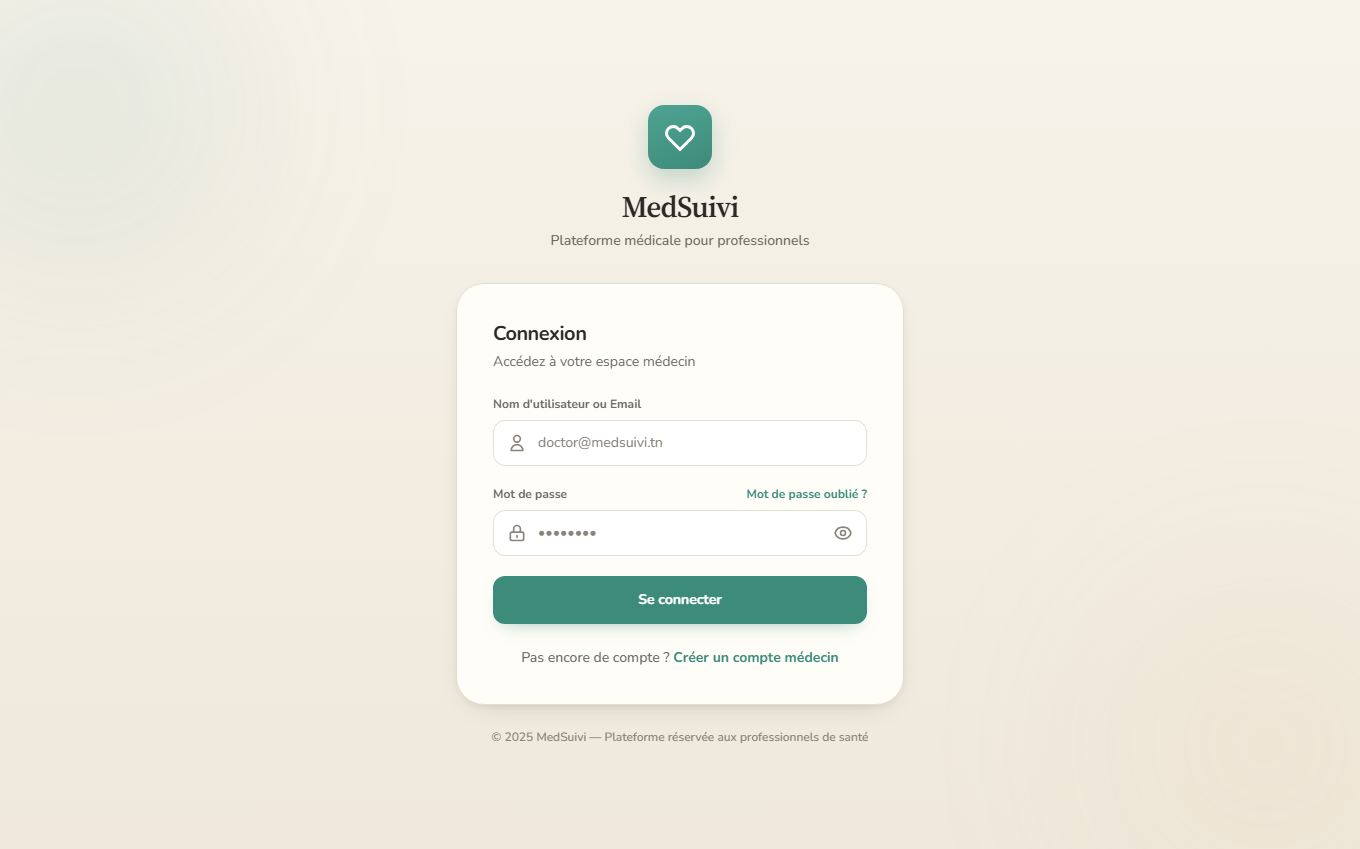
\includegraphics[width=0.8\textwidth]{rapport-screenshots/01-login.png}
  \caption{Écran de connexion --- Authentification du médecin}
  \label{fig:web-login}
\end{figure}

L'écran de connexion (Figure~\ref{fig:web-login}) permet au médecin de
s'authentifier via son identifiant ou adresse email et son mot de passe. Un
contrôle de rôle est effectué côté client : seuls les comptes de type
\texttt{MEDECIN} sont admis sur l'interface web.

% ─── Figure : Inscription médecin ─────────────────────────────────────
\begin{figure}[H]
  \centering
  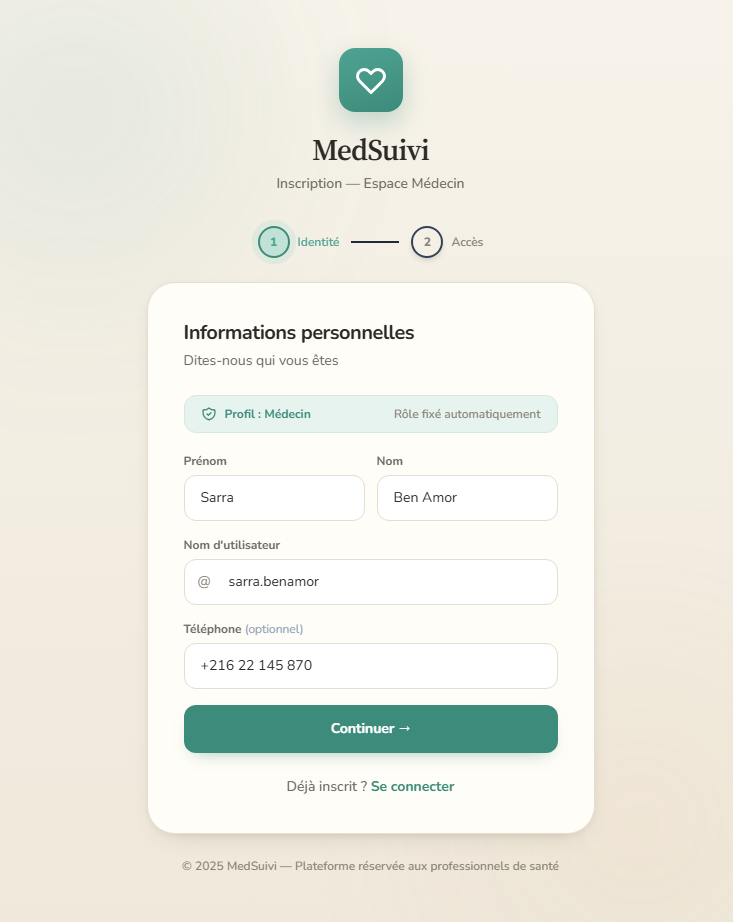
\includegraphics[width=0.8\textwidth]{rapport-screenshots/03-register-step1.png}
  \caption{Inscription du médecin --- Étape 1 : identité}
  \label{fig:web-register1}
\end{figure}

% ─── Figure : Inscription médecin (étape 2) ───────────────────────────
\begin{figure}[H]
  \centering
  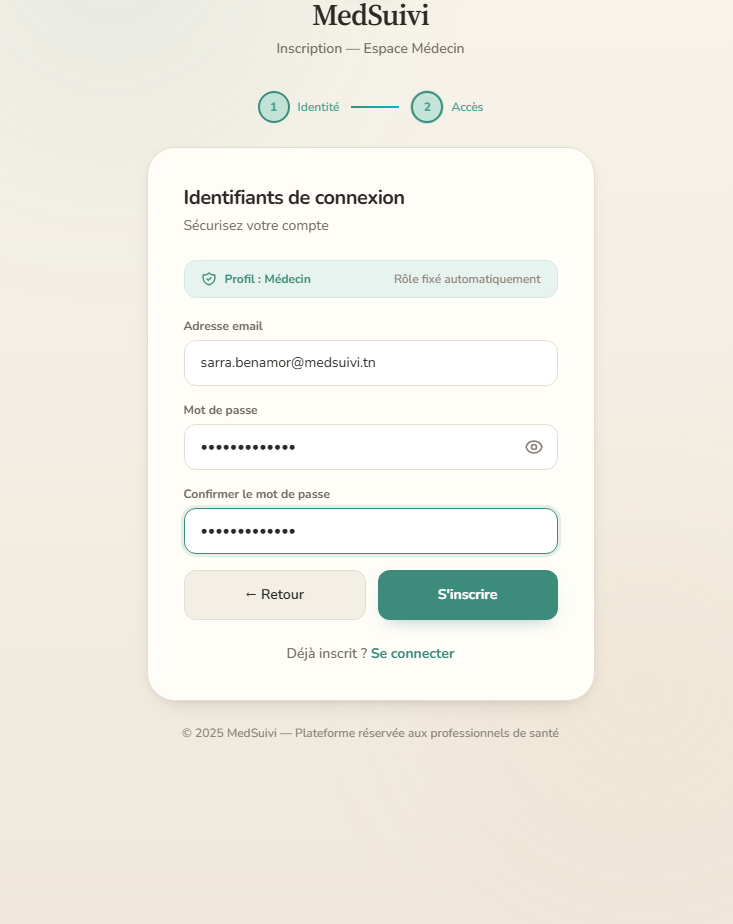
\includegraphics[width=0.8\textwidth]{rapport-screenshots/04-register-step2.png}
  \caption{Inscription du médecin --- Étape 2 : identifiants de connexion}
  \label{fig:web-register2}
\end{figure}

L'inscription d'un médecin (Figures~\ref{fig:web-register1}
et~\ref{fig:web-register2}) s'effectue en deux étapes : la saisie des
informations personnelles (prénom, nom, nom d'utilisateur, téléphone) puis la
définition des identifiants de connexion (email et mot de passe robuste). Le
rôle \texttt{MEDECIN} est fixé automatiquement par l'application.

% ─── Figure : Mot de passe oublié ─────────────────────────────────────
\begin{figure}[H]
  \centering
  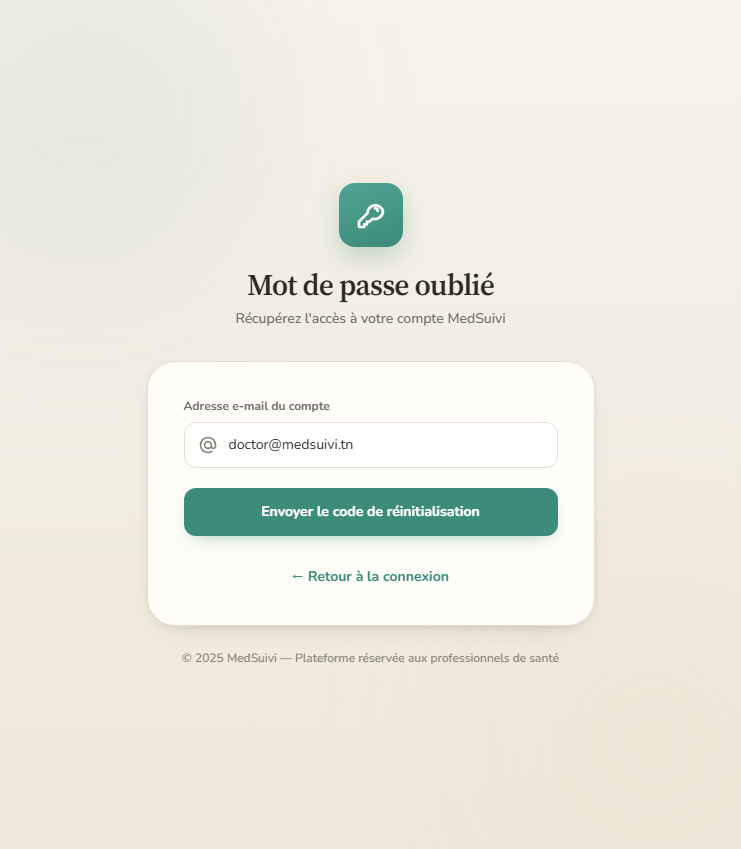
\includegraphics[width=0.8\textwidth]{rapport-screenshots/05-forgot-password.png}
  \caption{Mot de passe oublié --- Demande du code de réinitialisation}
  \label{fig:web-forgot}
\end{figure}

% ─── Figure : Réinitialisation ────────────────────────────────────────
\begin{figure}[H]
  \centering
  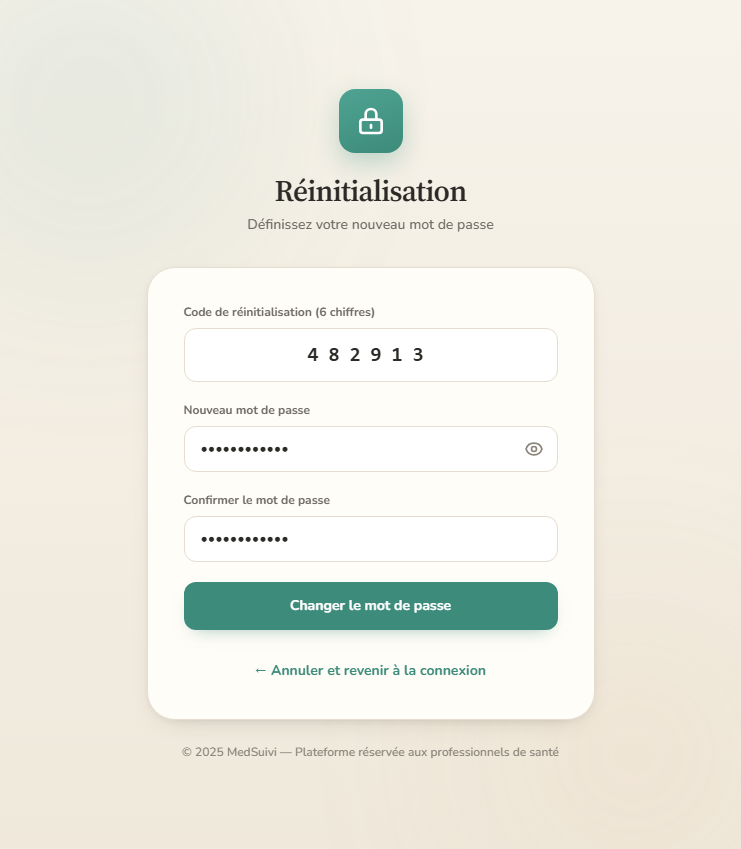
\includegraphics[width=0.8\textwidth]{rapport-screenshots/06-reset-password.png}
  \caption{Réinitialisation --- Définition du nouveau mot de passe}
  \label{fig:web-reset}
\end{figure}

Le parcours de récupération de compte (Figures~\ref{fig:web-forgot}
et~\ref{fig:web-reset}) permet de demander un code de réinitialisation à six
chiffres par email, puis de définir un nouveau mot de passe respectant la
politique de robustesse (huit caractères minimum, une majuscule, un chiffre).

% ─── Figure : Vue d'ensemble ──────────────────────────────────────────
\begin{figure}[H]
  \centering
  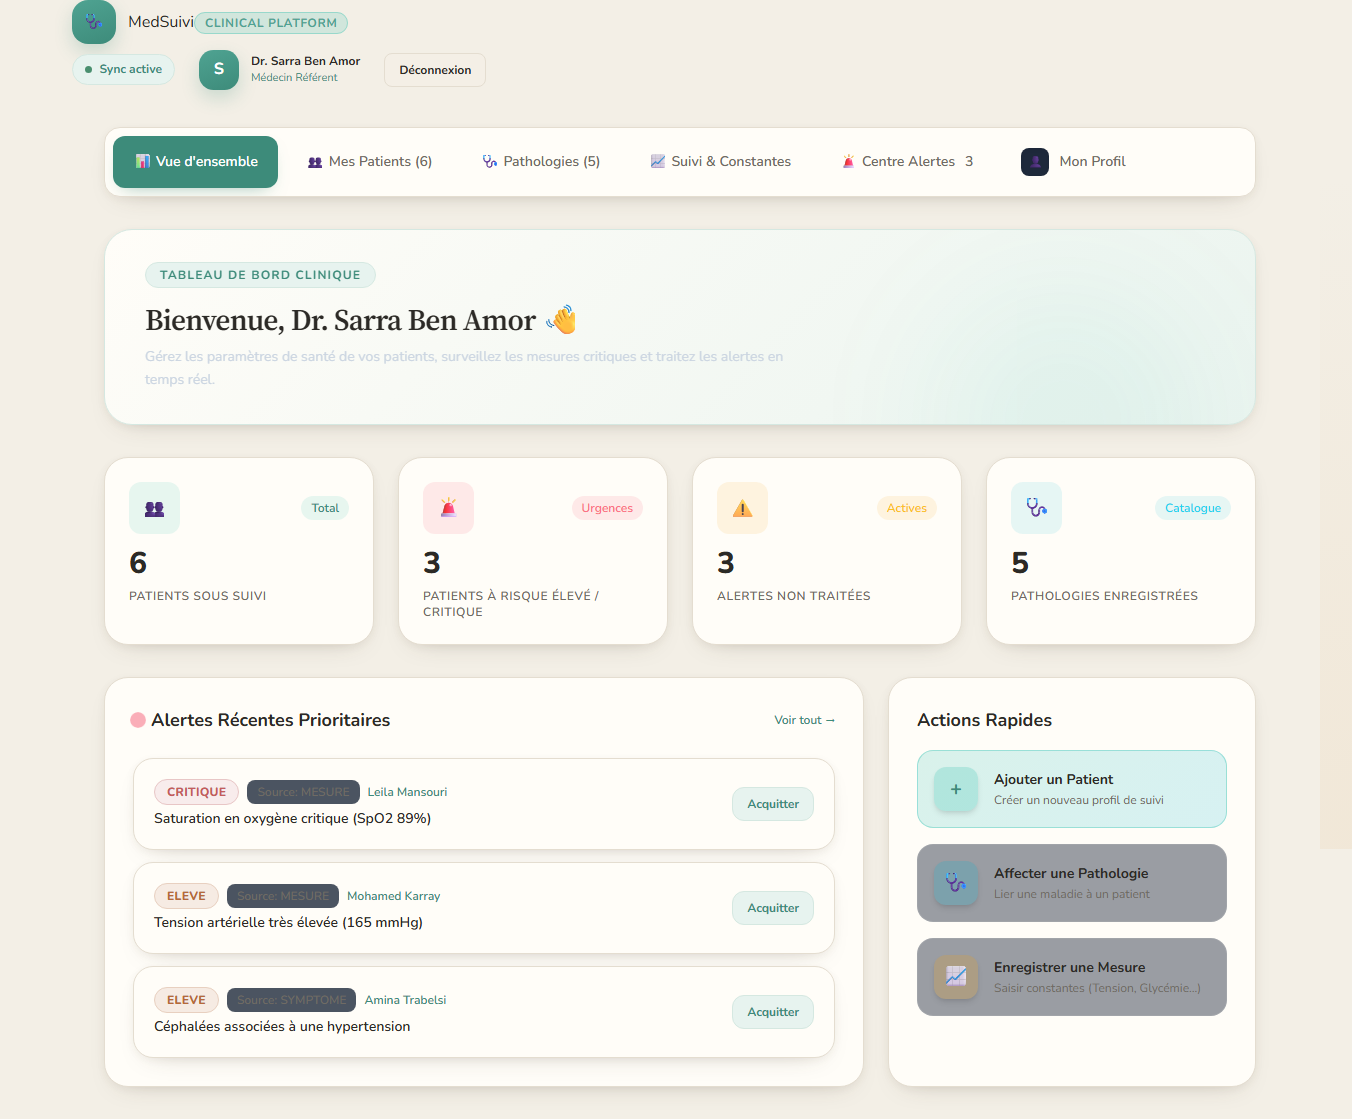
\includegraphics[width=0.8\textwidth]{rapport-screenshots/07-dashboard-overview.png}
  \caption{Tableau de bord médecin --- Vue d'ensemble}
  \label{fig:web-overview}
\end{figure}

La vue d'ensemble (Figure~\ref{fig:web-overview}) affiche les indicateurs
synthétiques de l'activité (patients sous suivi, patients à risque élevé ou
critique, alertes non traitées, pathologies enregistrées), la liste des alertes
récentes prioritaires avec bouton d'acquittement, ainsi que des actions rapides
(ajouter un patient, affecter une pathologie, enregistrer une mesure).

% ─── Figure : Mes Patients ────────────────────────────────────────────
\begin{figure}[H]
  \centering
  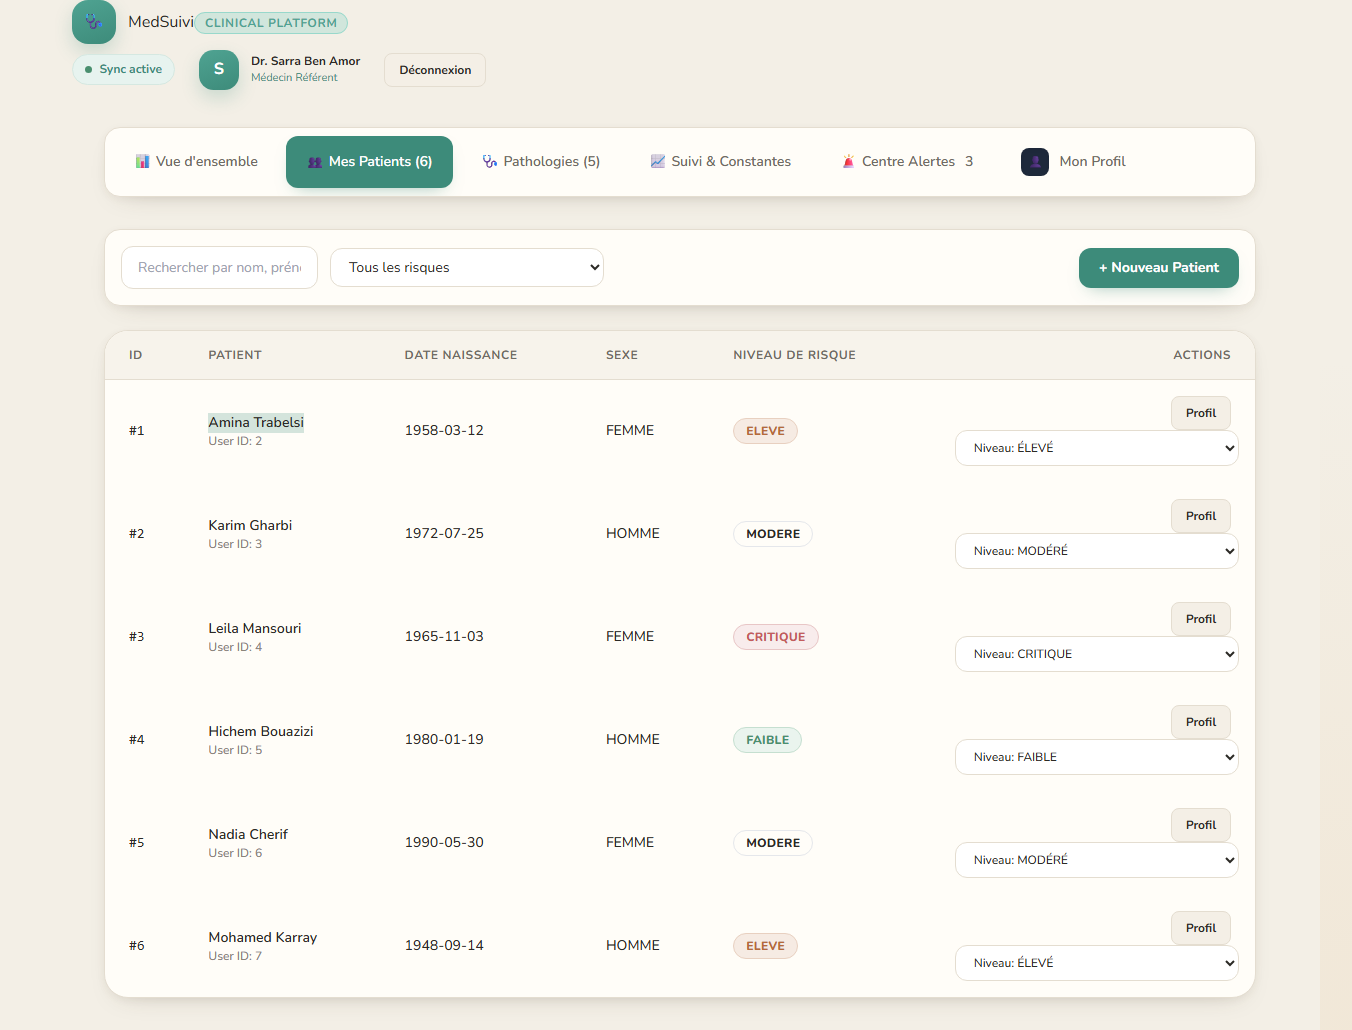
\includegraphics[width=0.8\textwidth]{rapport-screenshots/08-dashboard-patients.png}
  \caption{Onglet Mes Patients --- Liste, recherche et filtrage par risque}
  \label{fig:web-patients}
\end{figure}

L'onglet Mes Patients (Figure~\ref{fig:web-patients}) présente la liste des
patients suivis avec leur niveau de risque respectif. Une barre de recherche et
un filtre par niveau de risque permettent de retrouver rapidement un dossier ;
chaque ligne donne accès à la fiche détaillée du patient et à la modification
de son niveau de risque.

% ─── Figure : Fiche patient & moteur prédictif ────────────────────────
\begin{figure}[H]
  \centering
  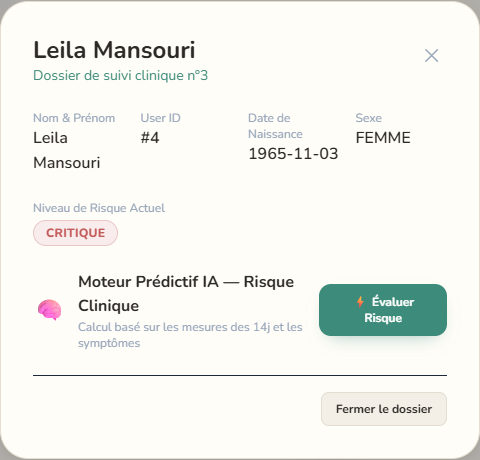
\includegraphics[width=0.6\textwidth]{rapport-screenshots/13-patient-fiche-predict.png}
  \caption{Fiche patient --- Dossier clinique et moteur prédictif IA}
  \label{fig:web-fiche}
\end{figure}

La fiche patient (Figure~\ref{fig:web-fiche}) regroupe les informations
d'identité du patient (nom, prénom, identifiant utilisateur, date de naissance,
sexe) ainsi que son niveau de risque actuel. Elle intègre le moteur prédictif
IA de gravité, accompagné du bouton \textit{« Évaluer Risque »} qui interroge le
micro-service d'analyse (\textit{Predict API}).

% ─── Figure : Résultat de prédiction IA ───────────────────────────────
\begin{figure}[H]
  \centering
  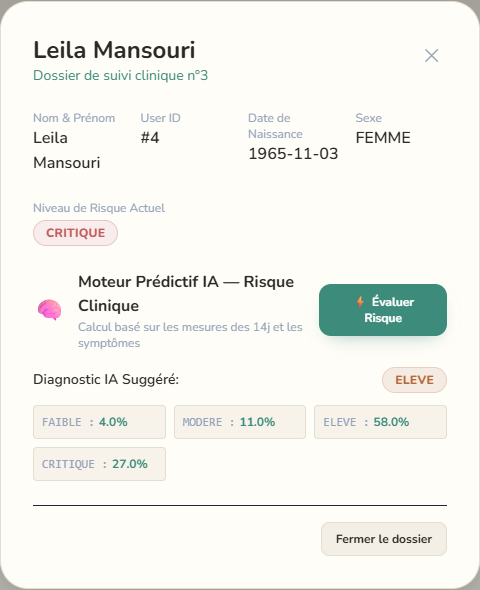
\includegraphics[width=0.6\textwidth]{rapport-screenshots/14-predict-result.png}
  \caption{Prédiction IA --- Gravité suggérée et probabilités par classe}
  \label{fig:web-predict}
\end{figure}

Après lancement de l'analyse (Figure~\ref{fig:web-predict}), le moteur prédictif
retourne la gravité suggérée (ici \texttt{ELEVE}) ainsi que la distribution de
probabilité sur les quatre classes de risque (\texttt{FAIBLE}, \texttt{MODERE},
\texttt{ELEVE}, \texttt{CRITIQUE}), permettant au médecin d'étayer sa décision
clinique.

% ─── Figure : Pathologies ─────────────────────────────────────────────
\begin{figure}[H]
  \centering
  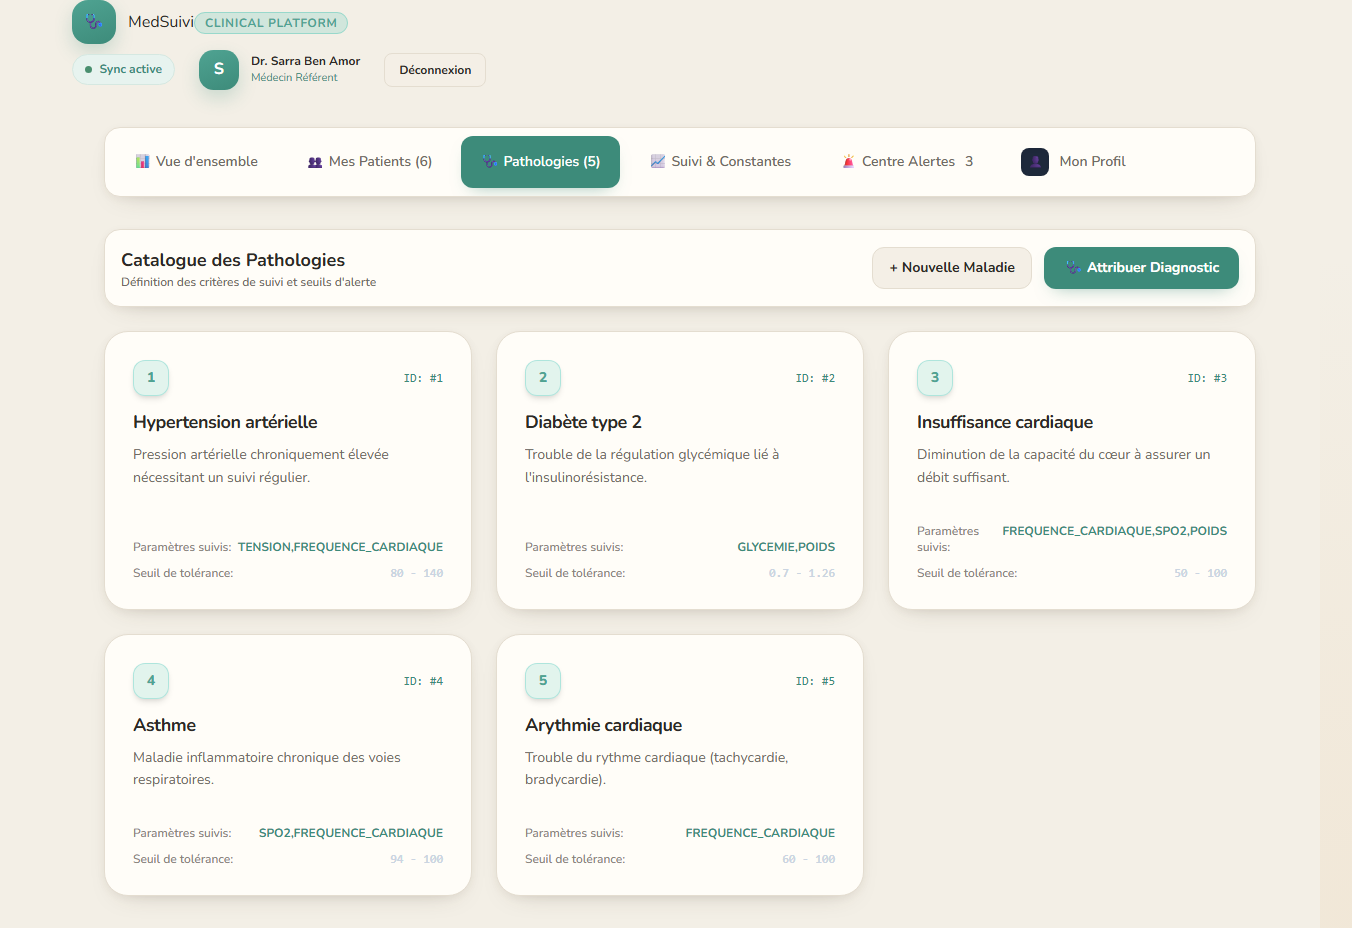
\includegraphics[width=0.8\textwidth]{rapport-screenshots/09-dashboard-pathologies.png}
  \caption{Onglet Pathologies --- Catalogue et seuils de tolérance}
  \label{fig:web-pathologies}
\end{figure}

L'onglet Pathologies (Figure~\ref{fig:web-pathologies}) regroupe le catalogue
des maladies suivies par la plateforme, avec pour chacune les paramètres
surveillés et les seuils de tolérance utilisés pour générer les alertes. Le
médecin peut y créer une nouvelle pathologie ou affecter un diagnostic à un
patient.

% ─── Figure : Suivi & Constantes ──────────────────────────────────────
\begin{figure}[H]
  \centering
  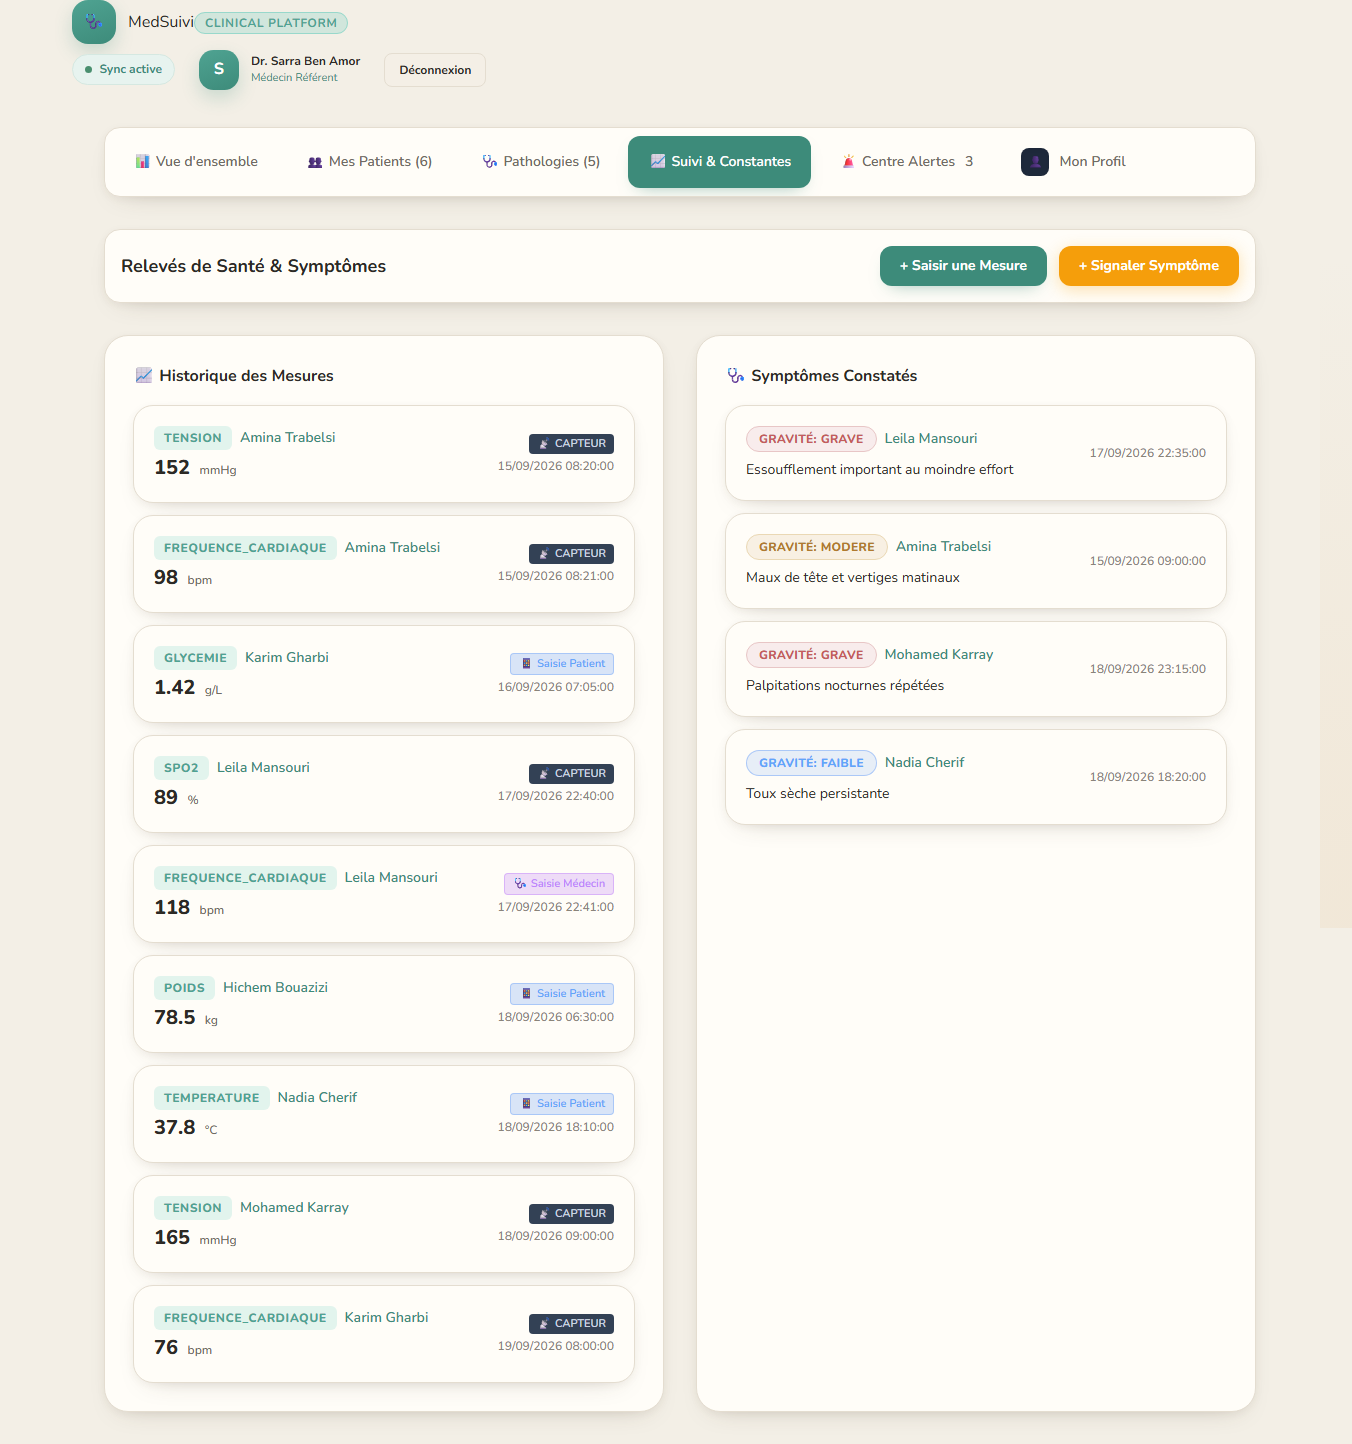
\includegraphics[width=0.8\textwidth]{rapport-screenshots/10-dashboard-suivi.png}
  \caption{Onglet Suivi \& Constantes --- Mesures et symptômes}
  \label{fig:web-suivi}
\end{figure}

L'onglet Suivi \& Constantes (Figure~\ref{fig:web-suivi}) centralise l'historique
des mesures enregistrées (tension, glycémie, fréquence cardiaque, température,
poids, SpO2) avec leur source (capteur, saisie patient ou saisie médecin), ainsi
que les symptômes constatés classés par gravité.

% ─── Figure : Centre Alertes ──────────────────────────────────────────
\begin{figure}[H]
  \centering
  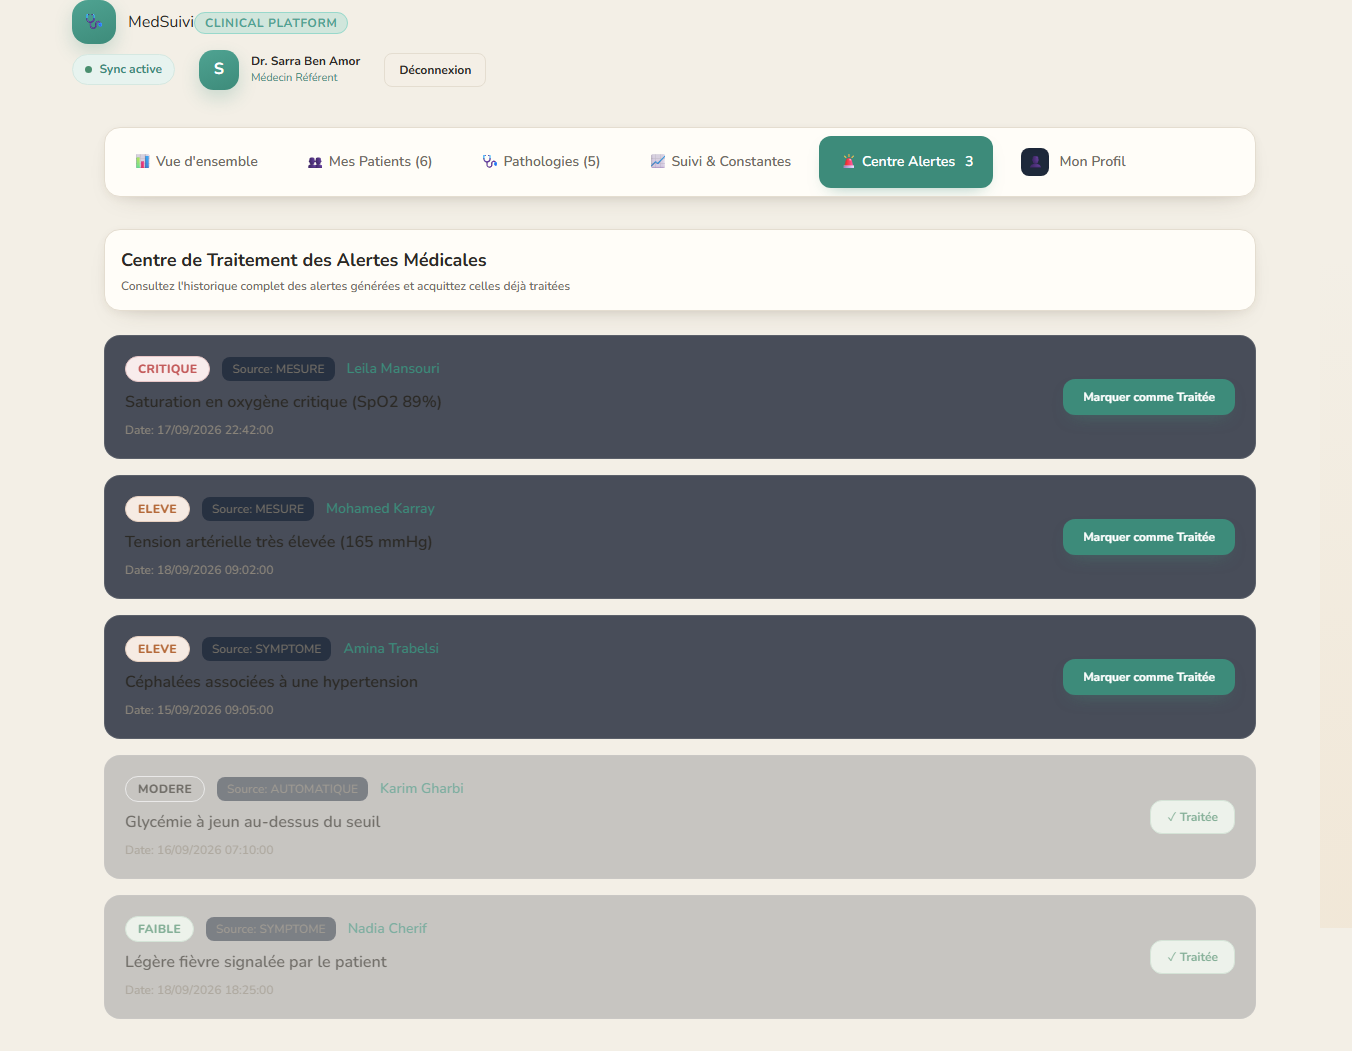
\includegraphics[width=0.8\textwidth]{rapport-screenshots/11-dashboard-alertes.png}
  \caption{Onglet Centre Alertes --- Traitement des alertes médicales}
  \label{fig:web-alertes}
\end{figure}

L'onglet Centre Alertes (Figure~\ref{fig:web-alertes}) liste l'ensemble des
alertes générées (par une mesure hors seuil, un symptôme ou automatiquement),
avec leur niveau de risque, leur source et leur date. Le médecin peut acquitter
chaque alerte une fois traitée.

% ─── Figure : Mon Profil ──────────────────────────────────────────────
\begin{figure}[H]
  \centering
  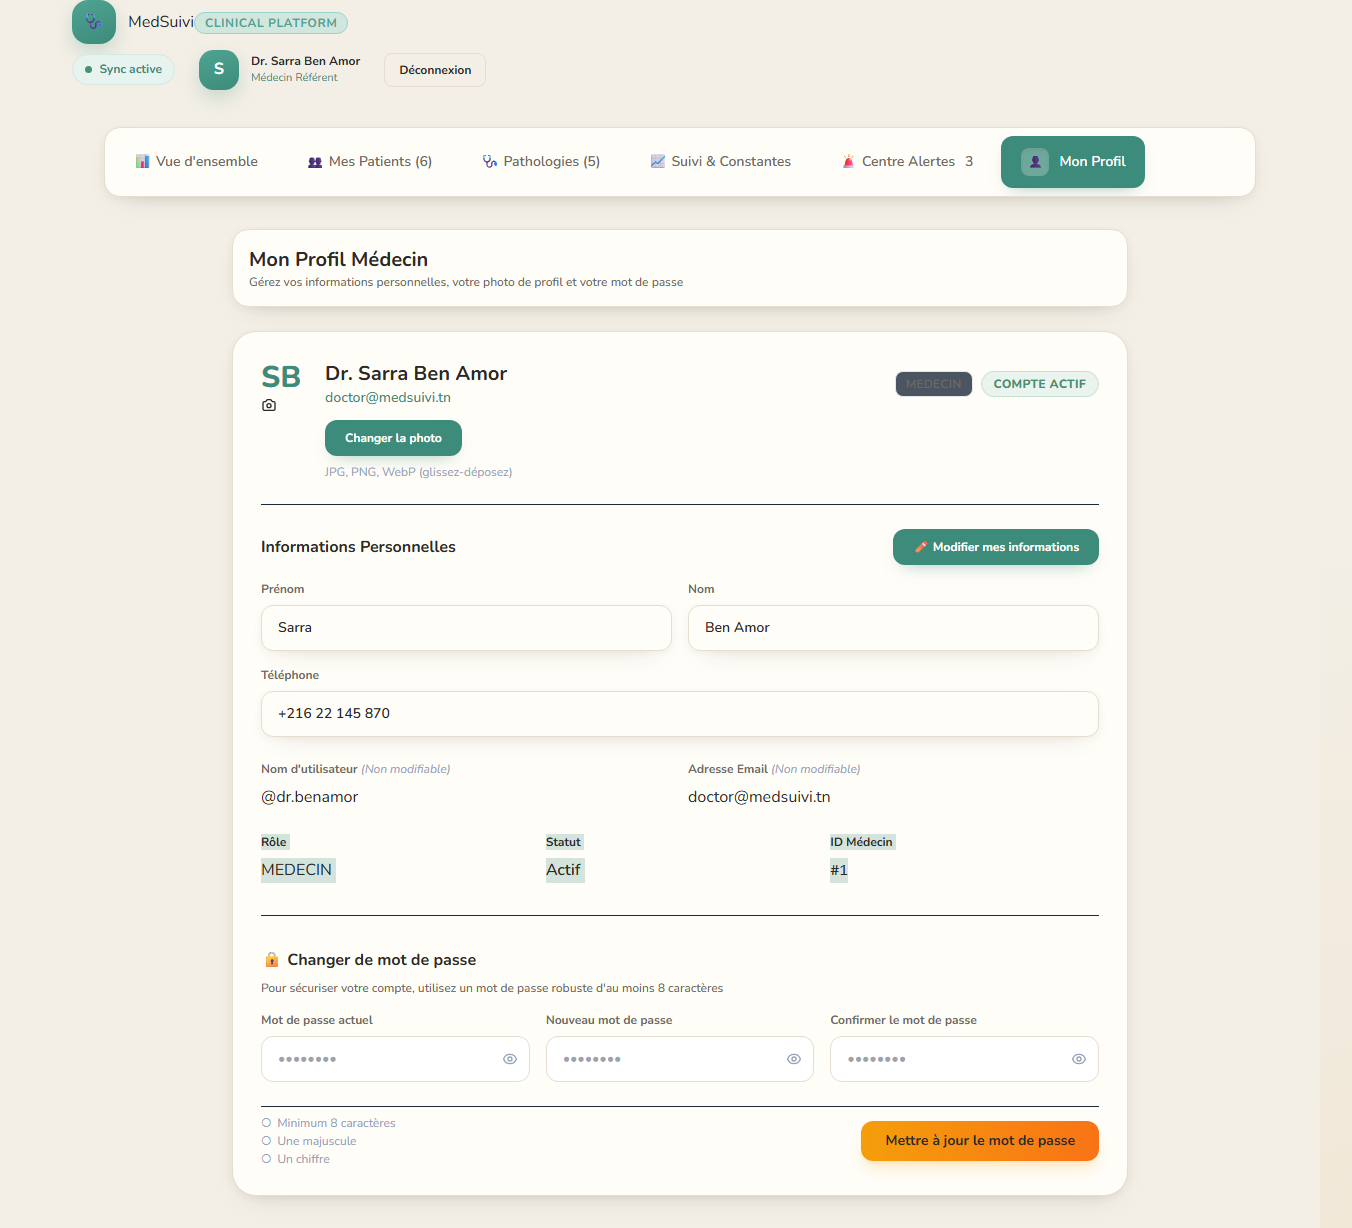
\includegraphics[width=0.8\textwidth]{rapport-screenshots/12-dashboard-profil.png}
  \caption{Onglet Mon Profil --- Informations, photo et mot de passe}
  \label{fig:web-profil}
\end{figure}

L'onglet Mon Profil (Figure~\ref{fig:web-profil}) permet au médecin de consulter
et modifier ses informations personnelles, de gérer sa photo de profil et de
changer son mot de passe, avec un indicateur de robustesse en temps réel.

% ─────────────────────────────────────────────────────────────
\subsection{Communication avec le back-end}
% ─────────────────────────────────────────────────────────────

Les deux clients (mobile et web) suivent le même patron d'interaction avec
le système :

\begin{enumerate}
  \item \textbf{Authentification} : obtention d'un jeton JWT auprès du
    micro-service d'authentification via l'API Gateway.
  \item \textbf{Appels authentifiés} : toutes les requêtes subséquentes
    transportent le jeton dans l'en-tête \texttt{Authorization: Bearer <token>}.
  \item \textbf{Gestion des erreurs} : les codes \texttt{401 Unauthorized}
    entraînent une invalidation locale de la session et une redirection vers
    l'écran de connexion.
  \item \textbf{Isolation des services} : les clients ignorent la topologie
    interne des micro-services ; ils n'adressent que l'API Gateway, qui se
    charge du routage.
\end{enumerate}

% ============================================================
\chapter{Sprint 1 : Authentification et gestion des comptes}

Le premier sprint pose les fondations transverses de la plateforme : création
des comptes, authentification par jeton JWT et gestion du profil utilisateur.
Ces briques, portées par le \texttt{user-service}, sont consommées par tous les
sprints suivants, tant côté web médecin que mobile patient.

\section{User stories du sprint}
\begin{itemize}[leftmargin=1.4em]
  \item En tant que médecin, je m'inscris et je me connecte au portail.
  \item En tant qu'utilisateur, je réinitialise mon mot de passe par e-mail.
  \item En tant que patient, je me connecte à l'application mobile.
  \item En tant qu'utilisateur, je mets à jour mon profil et ma photo.
\end{itemize}

\section{Diagramme de cas d'utilisation « s'authentifier »}
La figure~\ref{fig:uc-auth} cadre le périmètre d'authentification. Médecin et
patient partagent le même mécanisme fourni par le \texttt{user-service} ; le
cas « réinitialiser le mot de passe » est inclus dans le parcours
« mot de passe oublié ».

\begin{figure}[H]
  \centering
  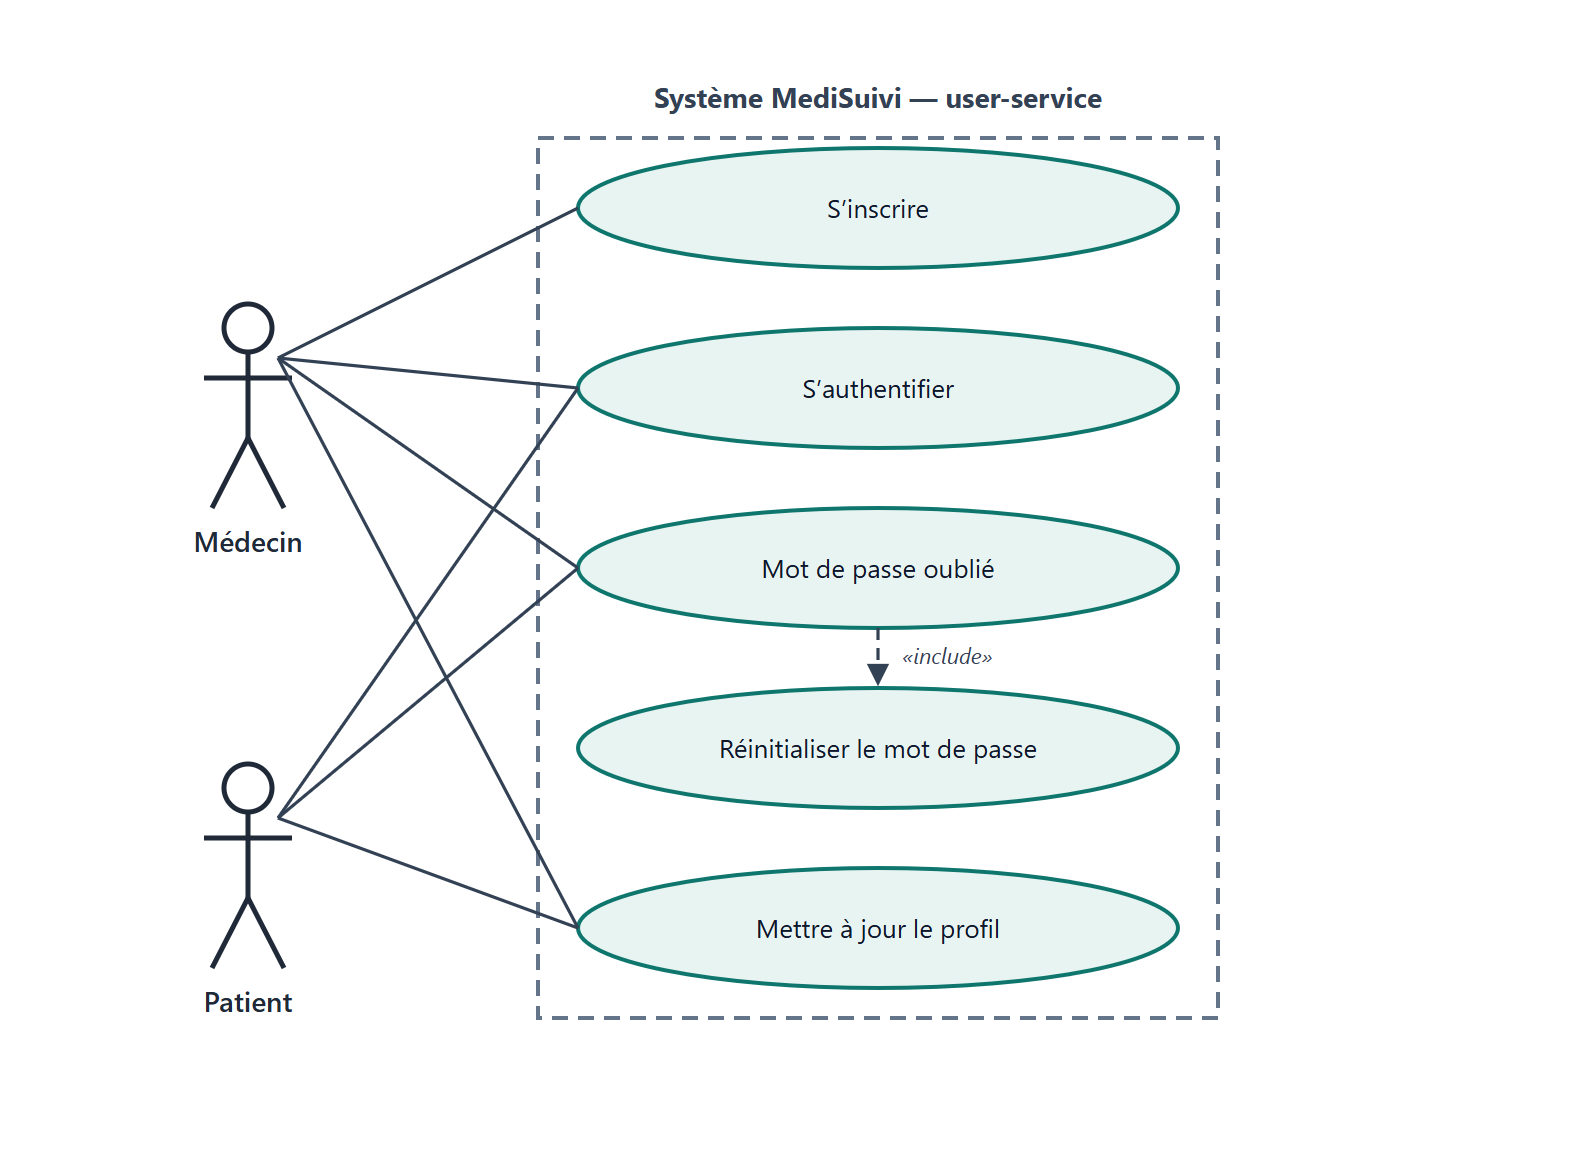
\includegraphics[width=0.75\textwidth]{rapport-screenshots/20-uc-auth.png}
  \caption{Diagramme de cas d'utilisation « s'authentifier »}
  \label{fig:uc-auth}
\end{figure}

\section{Diagramme de séquence système « s'authentifier »}
La figure~\ref{fig:seq-auth} détaille le scénario nominal de connexion : la
requête traverse la Gateway puis le \texttt{user-service}, qui vérifie les
identifiants en base avant de signer et renvoyer un jeton JWT.

\begin{figure}[H]
  \centering
  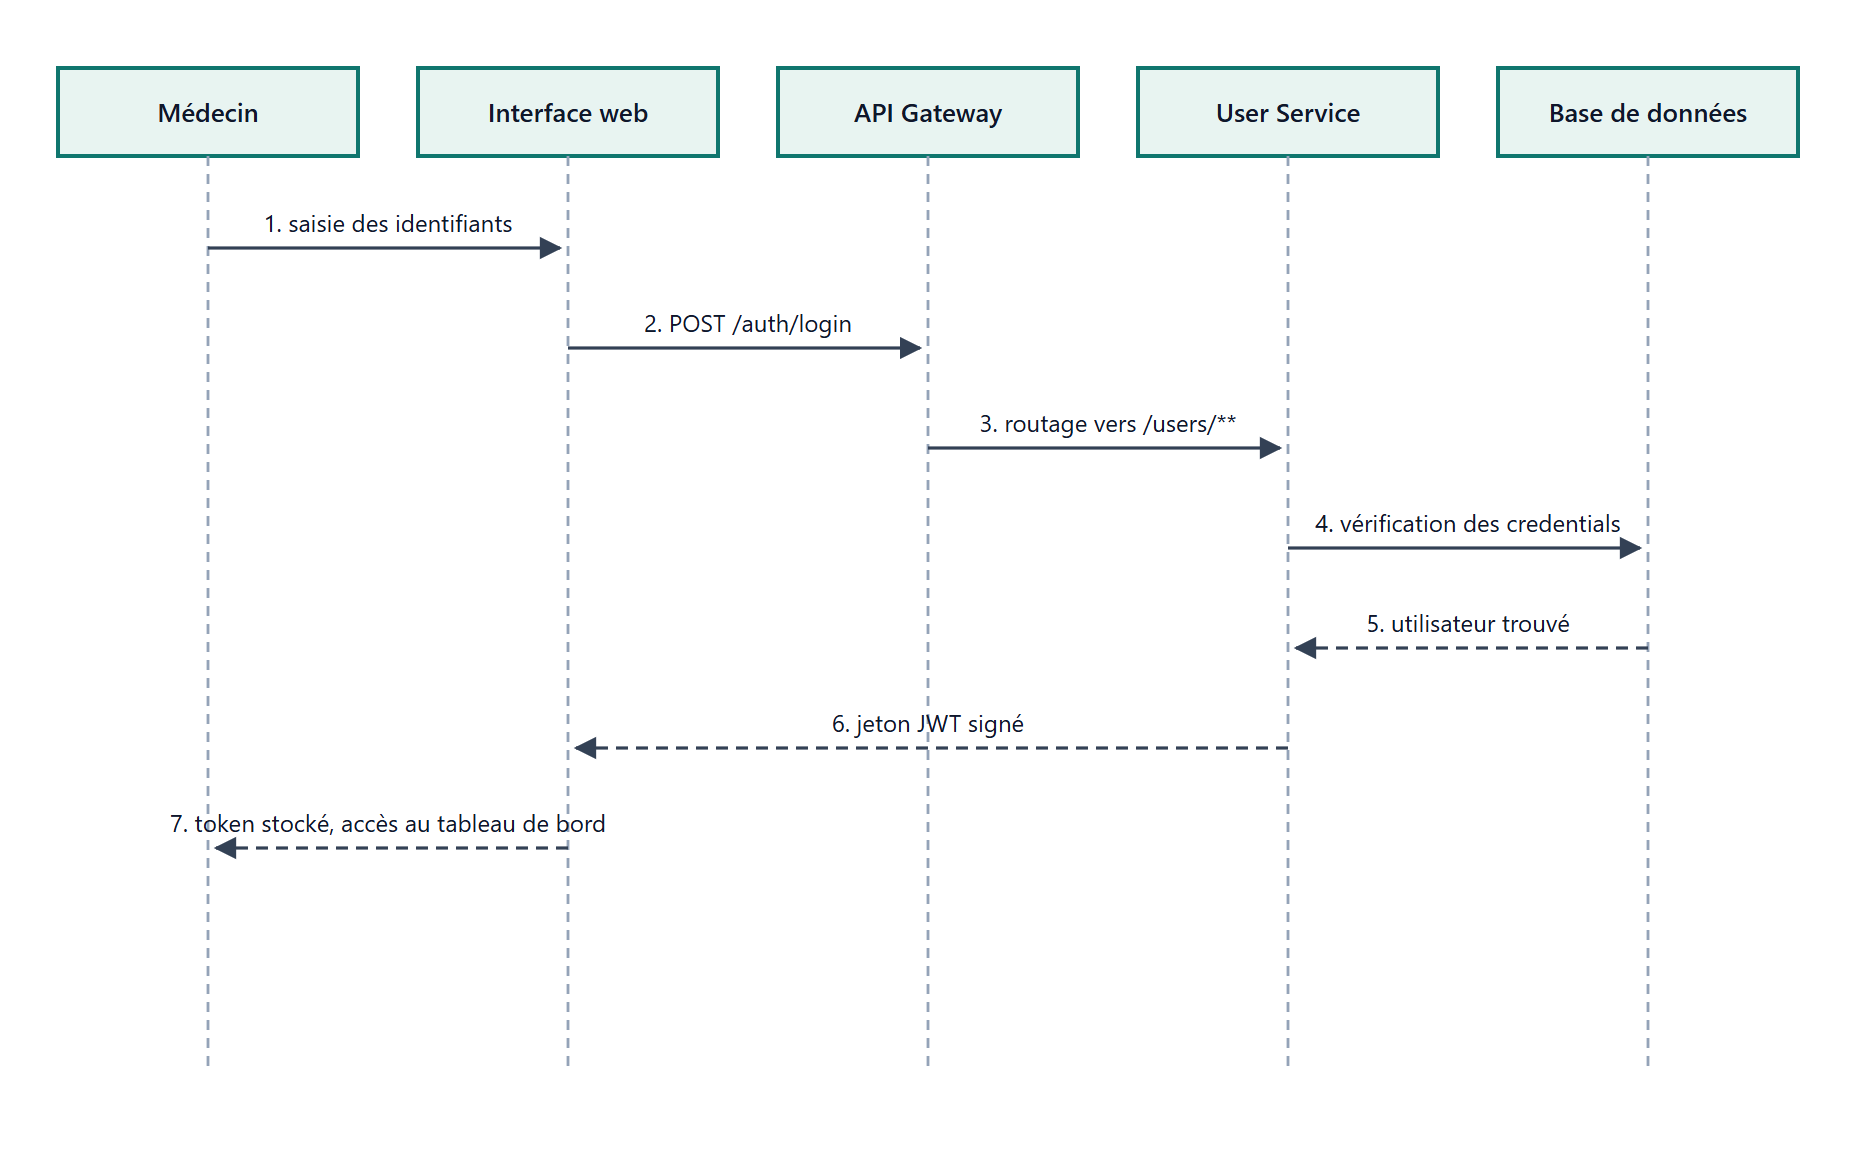
\includegraphics[width=0.92\textwidth]{rapport-screenshots/21-seq-auth.png}
  \caption{Diagramme de séquence système « s'authentifier »}
  \label{fig:seq-auth}
\end{figure}

\section{Diagramme de classes du Sprint 1}
La figure~\ref{fig:class-s1} présente les entités du sprint : le compte
\texttt{User}, son extension métier \texttt{Medecin} et le contrôleur
d'authentification qui orchestre inscription, connexion et réinitialisation.

\begin{figure}[H]
  \centering
  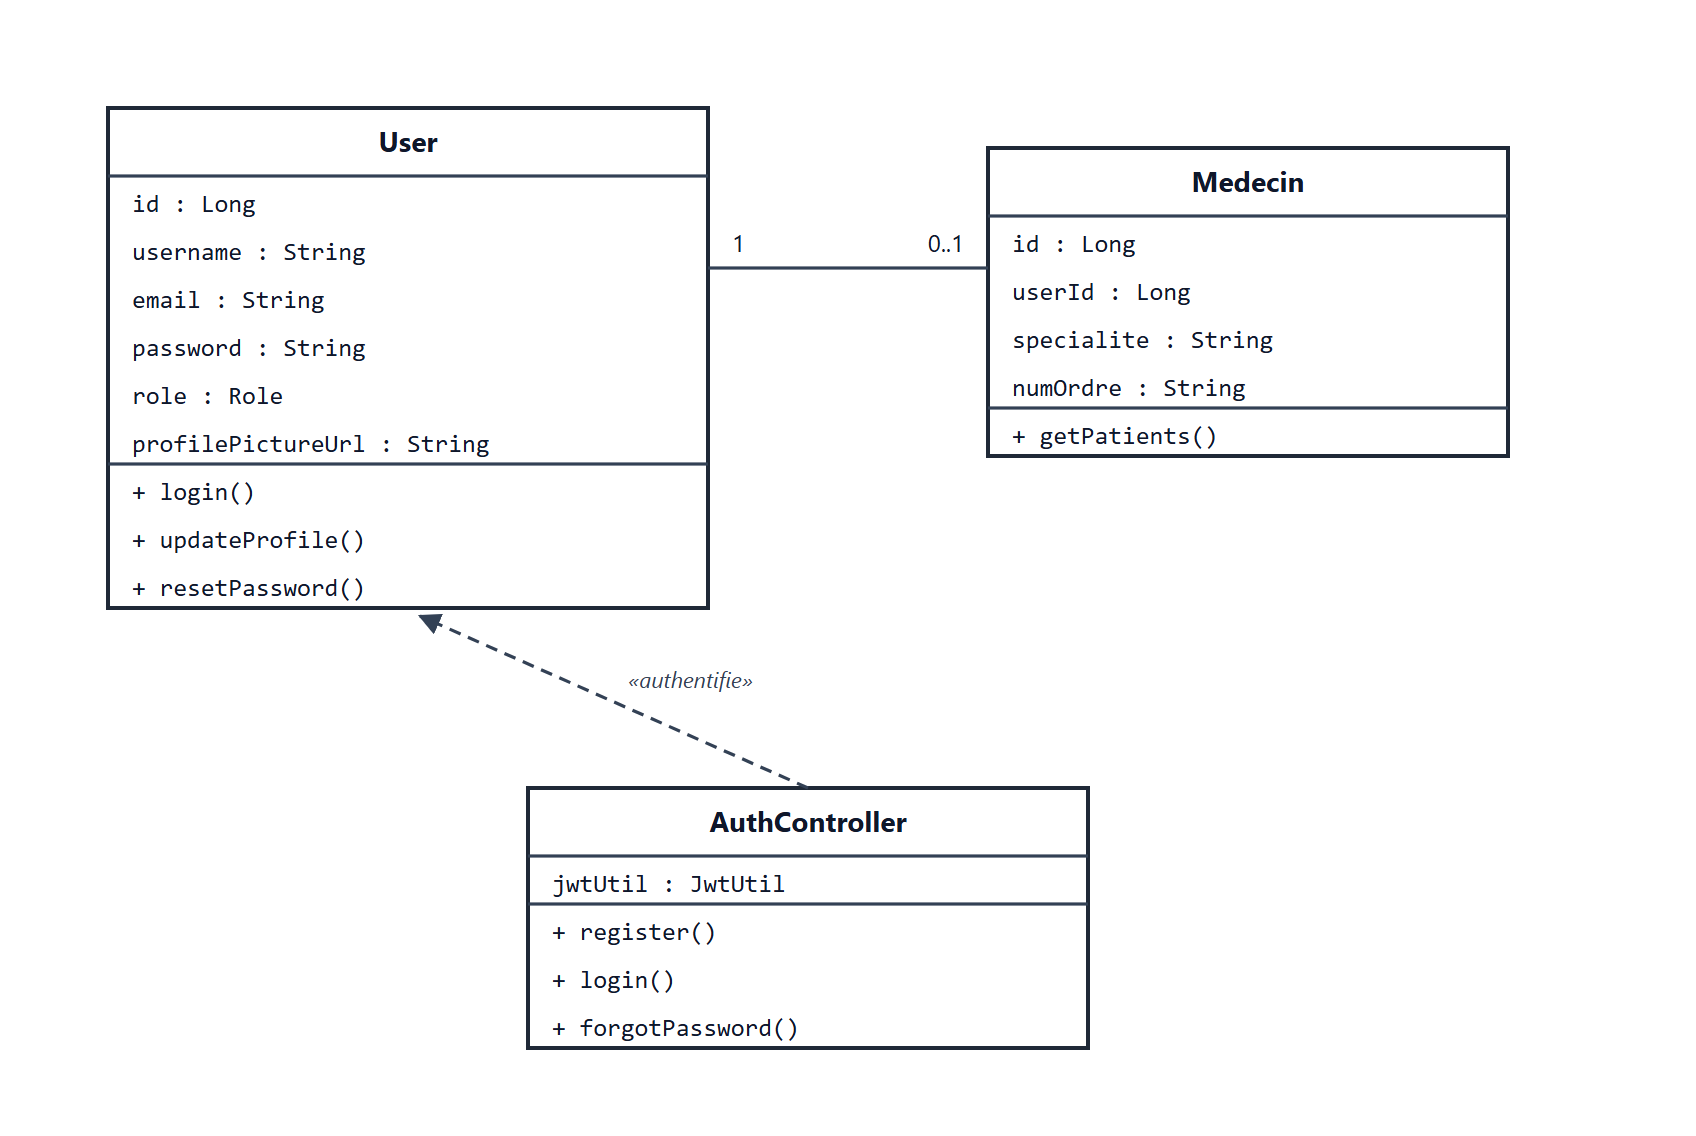
\includegraphics[width=0.8\textwidth]{rapport-screenshots/22-class-s1.png}
  \caption{Diagramme de classes du Sprint 1}
  \label{fig:class-s1}
\end{figure}

\section{Inscription d'un médecin}
L'inscription d'un médecin s'effectue en deux étapes (identité puis
identifiants de connexion) ; le rôle \texttt{MEDECIN} est positionné
automatiquement par l'application (figure~\ref{fig:ui-register}).

\begin{figure}[H]
  \centering
  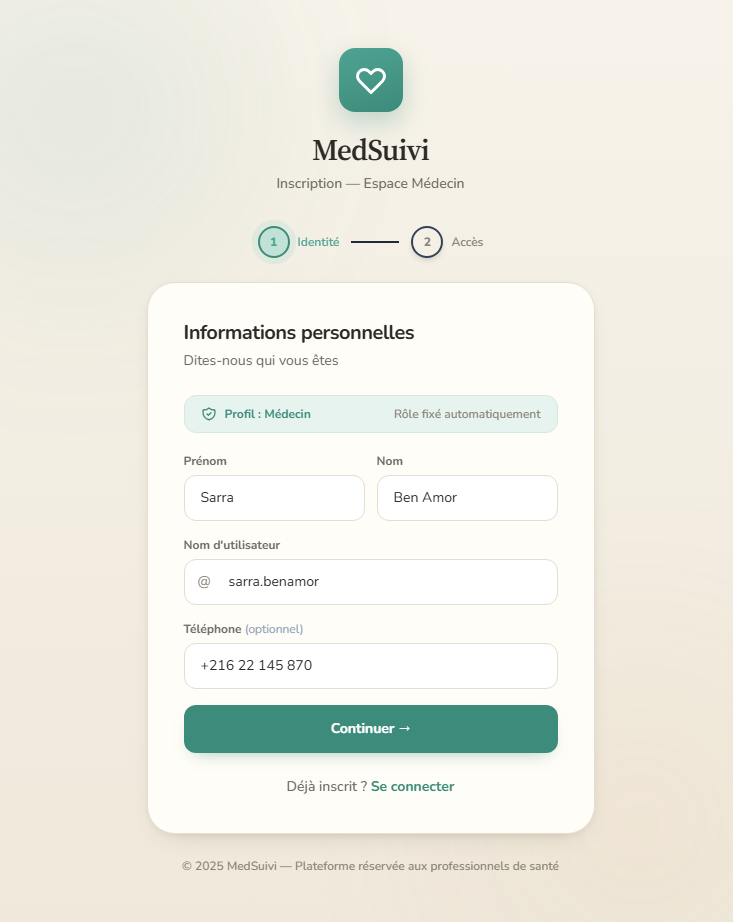
\includegraphics[width=0.8\textwidth]{rapport-screenshots/03-register-step1.png}
  \caption{Interface « inscription médecin »}
  \label{fig:ui-register}
\end{figure}

\section{Connexion (web et mobile)}
Le même compte utilisateur permet d'accéder au portail web
(figure~\ref{fig:ui-login}) ou à l'application mobile
(figure~\ref{fig:ui-login-mobile}) ; un contrôle de rôle oriente chaque client
vers son espace.

\begin{figure}[H]
  \centering
  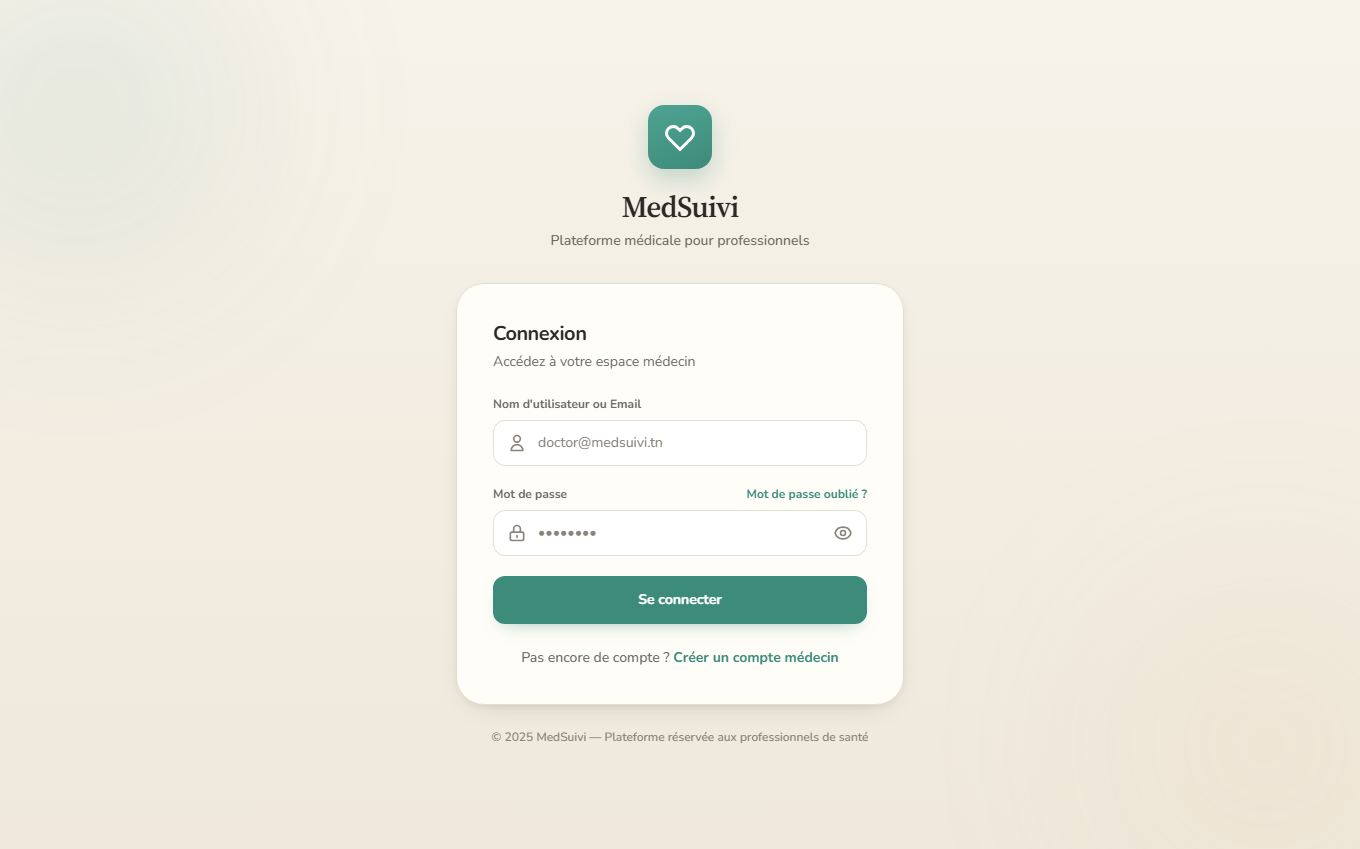
\includegraphics[width=0.8\textwidth]{rapport-screenshots/01-login.png}
  \caption{Interface « authentification » (web médecin)}
  \label{fig:ui-login}
\end{figure}

\begin{figure}[H]
  \centering
  
\includegraphics[width=0.4\textwidth]{login.png}
  \caption{Interface connexion mobile patient}
  \label{fig:ui-login-mobile}
\end{figure}

\section{Mot de passe oublié et réinitialisation}
Le parcours de récupération comprend une demande de code par e-mail
(figure~\ref{fig:ui-forgot}) puis la définition d'un nouveau mot de passe
robuste (figure~\ref{fig:ui-reset}).

\begin{figure}[H]
  \centering
  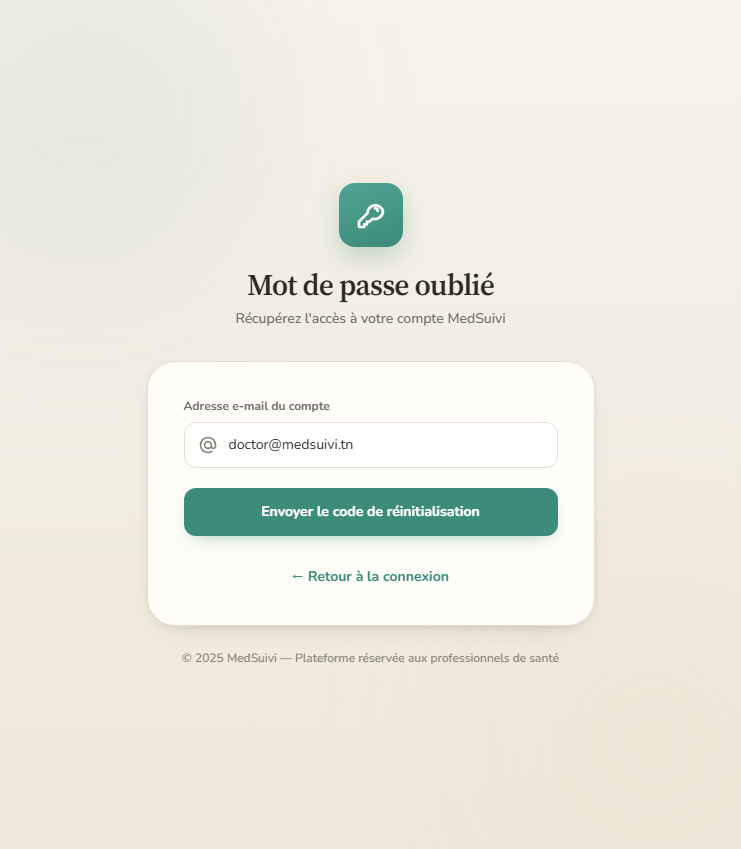
\includegraphics[width=0.8\textwidth]{rapport-screenshots/05-forgot-password.png}
  \caption{Interface authentification (mot de passe oublié)}
  \label{fig:ui-forgot}
\end{figure}

\begin{figure}[H]
  \centering
  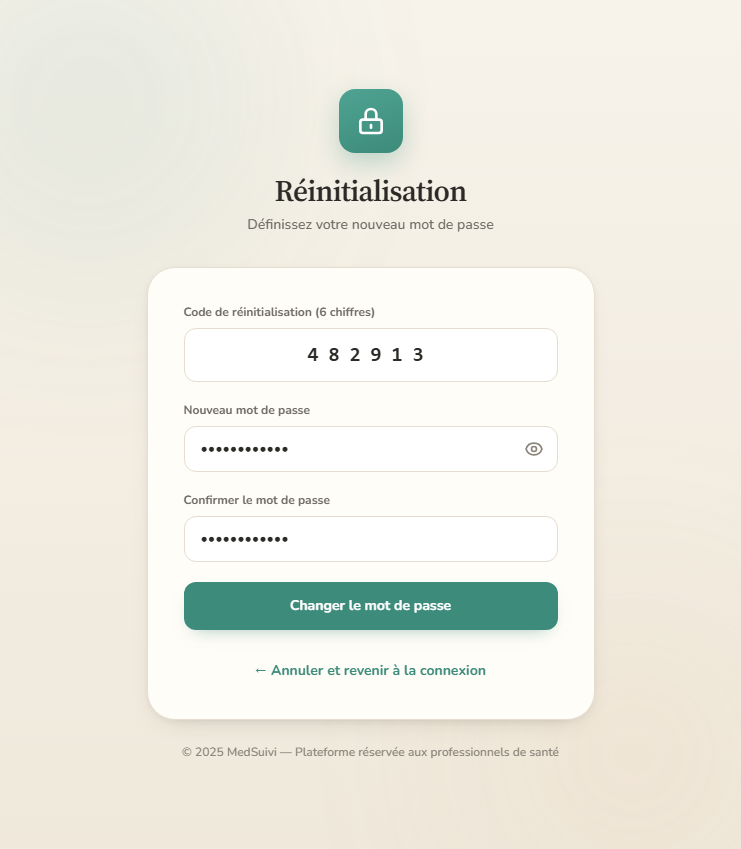
\includegraphics[width=0.8\textwidth]{rapport-screenshots/06-reset-password.png}
  \caption{Interface « réinitialisation du mot de passe »}
  \label{fig:ui-reset}
\end{figure}

\section{Mise à jour du profil et photo}
L'onglet « Mon Profil » du tableau de bord permet de modifier les informations
personnelles et de téléverser ou supprimer une photo de profil
(figure~\ref{fig:ui-profil}).

\begin{figure}[H]
  \centering
  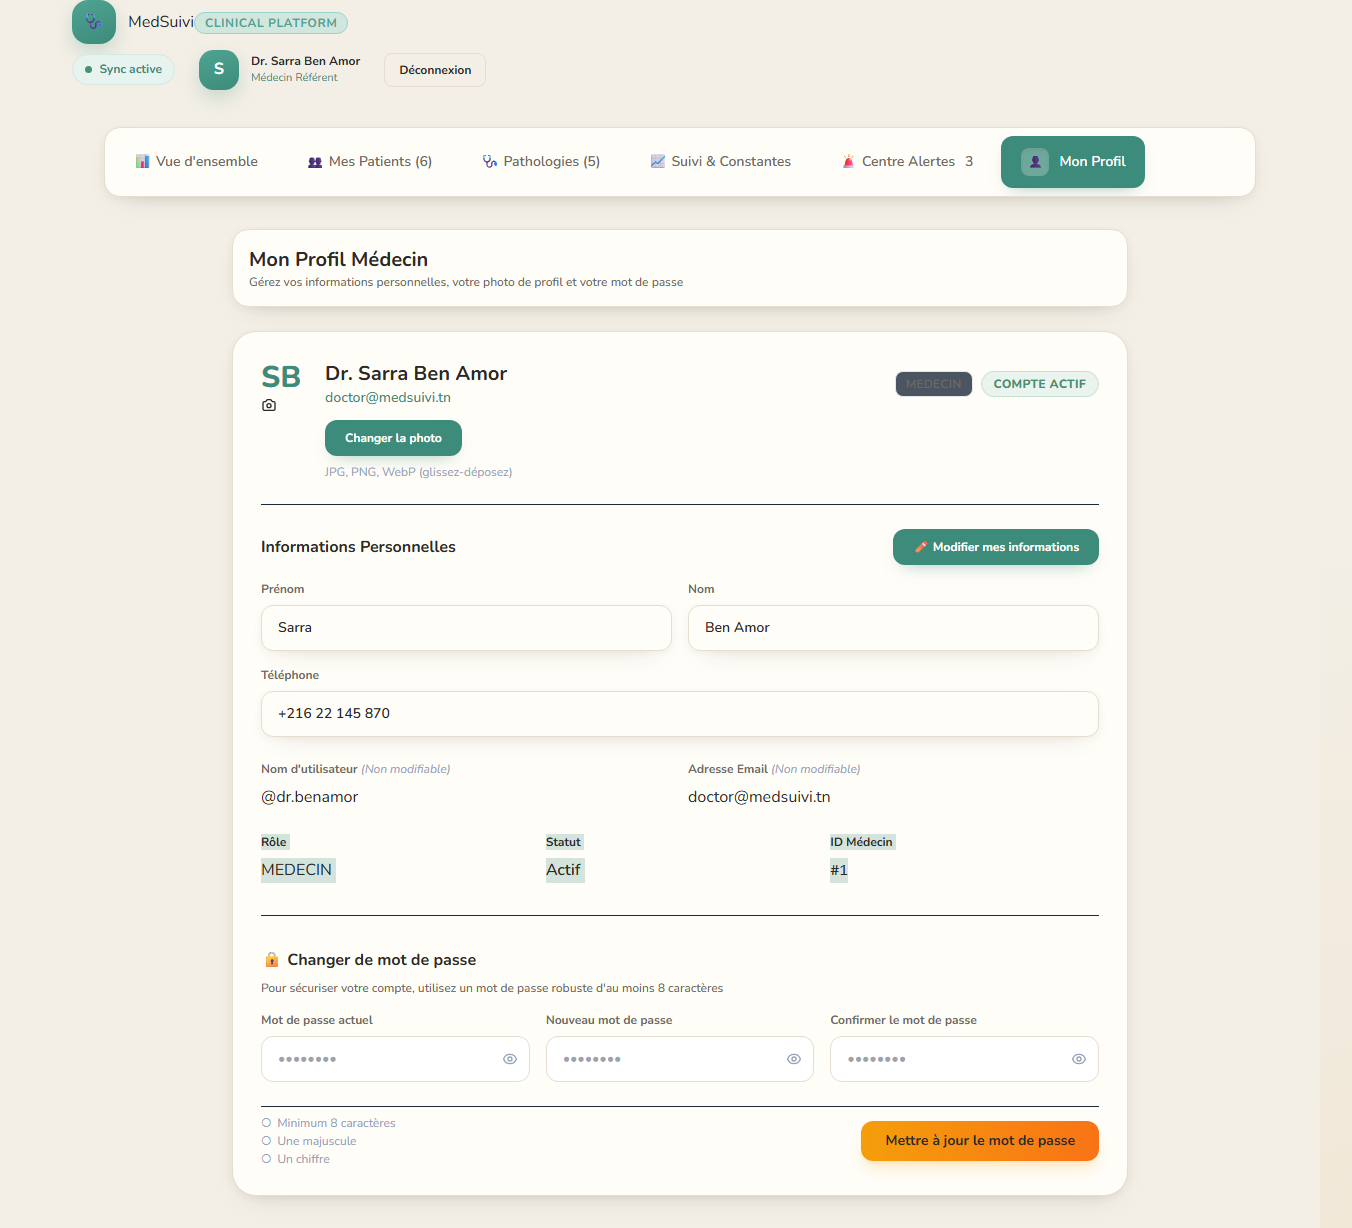
\includegraphics[width=0.8\textwidth]{rapport-screenshots/12-dashboard-profil.png}
  \caption{Interface « mise à jour du profil »}
  \label{fig:ui-profil}
\end{figure}

\section{Sécurité JWT et routes protégées}
Les routes du dashboard web et de l'espace mobile authentifié s'appuient sur un
jeton JWT délivré par le \texttt{user-service} ; chaque appel ultérieur via la
Gateway présente ce jeton dans l'en-tête \texttt{Authorization}.

% ============================================================
\chapter{Sprint 2 : Gestion des patients et des pathologies}

Ce sprint outille le médecin dans la constitution de sa patientèle : vue
d'ensemble de l'activité, CRUD des patients, catalogue de pathologies et
affectation d'un diagnostic à un patient.

\section{User stories du sprint}
\begin{itemize}[leftmargin=1.4em]
  \item En tant que médecin, je consulte la vue d'ensemble de mon activité.
  \item En tant que médecin, j'ajoute, modifie et recherche mes patients.
  \item En tant que médecin, je gère le catalogue de maladies.
  \item En tant que médecin, j'affecte une pathologie à un patient.
\end{itemize}

\section{Diagramme de cas d'utilisation « Gestion des patients »}
La figure~\ref{fig:uc-patients} regroupe les cas d'utilisation du sprint ;
l'affectation d'une pathologie réutilise à la fois la patientèle et le
catalogue de maladies.

\begin{figure}[H]
  \centering
  \begin{tikzpicture}[font=\small, >=Stealth]
    \draw[umlsys] (-1.1,-3.3) rectangle (4.9,3.1);
    \node[font=\small\bfseries] at (1.9,2.75) {Système MediSuivi --- \texttt{patient-service}};
    \umlactor{med}{-3.3,0}{Médecin}
    \node[uc] (ucvue)  at (1.9,1.9)  {Consulter la vue d'ensemble};
    \node[uc] (ucpat)  at (1.9,0.6)  {Gérer mes patients};
    \node[uc] (ucmal)  at (1.9,-0.7) {Gérer le catalogue de maladies};
    \node[uc] (ucaff)  at (1.9,-2.1) {Affecter une pathologie};
    \draw (med) -- (ucvue.west);
    \draw (med) -- (ucpat.west);
    \draw (med) -- (ucmal.west);
    \draw (med) -- (ucaff.west);
    \draw[->, dashed] (ucaff.west) to[out=200, in=200] node[left, font=\scriptsize]{«include»} (ucmal.west);
    \draw[->, dashed] (ucaff.west) to[out=210, in=210] node[left, font=\scriptsize]{«include»} (ucpat.west);
  \end{tikzpicture}
  \caption{Diagramme de cas d'utilisation « Gestion des patients »}
  \label{fig:uc-patients}
\end{figure}

\section{Diagramme de séquence « création d'un patient »}
La création d'un patient (figure~\ref{fig:seq-patient}) combine deux appels :
la création du compte utilisateur de type \texttt{PATIENT} puis
l'enregistrement de la fiche clinique liée à ce compte.

\begin{figure}[H]
  \centering
  \begin{tikzpicture}[font=\small, >=Stealth]
    \node[seqobj] (m)  at (0,0)    {Médecin};
    \node[seqobj] (web) at (3.2,0) {Interface web};
    \node[seqobj] (gw) at (6.4,0)  {API Gateway};
    \node[seqobj] (ps) at (9.6,0)  {Patient Service};
    \node[seqobj] (us) at (12.8,0) {User Service};
    \foreach \n in {m,web,gw,ps,us} { \draw[dashed] (\n.south) -- ++(0,-7.0); }
    \draw[->] (0,-1.0) -- node[above, font=\scriptsize]{1. formulaire nouveau patient} (3.2,-1.0);
    \draw[->] (3.2,-1.8) -- node[above, font=\scriptsize]{2. POST /patients} (6.4,-1.8);
    \draw[->] (6.4,-2.6) -- node[above, font=\scriptsize]{3. routage vers /patients/**} (9.6,-2.6);
    \draw[->] (9.6,-3.4) -- node[above, font=\scriptsize]{4. POST /users (rôle PATIENT)} (12.8,-3.4);
    \draw[->, dashed] (12.8,-4.2) -- node[above, font=\scriptsize]{5. compte créé} (9.6,-4.2);
    \draw[->] (9.6,-5.0) -- ++(1.1,0) |- node[above right, font=\scriptsize]{6. fiche patient + lien user} (9.6,-5.6);
    \draw[->, dashed] (9.6,-6.2) -- node[above, font=\scriptsize]{7. 201 Created} (3.2,-6.2);
    \draw[->, dashed] (3.2,-6.8) -- node[above, font=\scriptsize]{8. liste des patients actualisée} (0,-6.8);
  \end{tikzpicture}
  \caption{Diagramme de séquence « création d'un patient »}
  \label{fig:seq-patient}
\end{figure}

\section{Diagramme de classes du Sprint 2}
La figure~\ref{fig:class-s2} modélise la patientèle : un médecin suit plusieurs
patients, et l'association \texttt{PatientMaladie} porte la date du diagnostic
entre un patient et une pathologie du catalogue.

\begin{figure}[H]
  \centering
  \begin{tikzpicture}[font=\small, >=Stealth]
    \begin{scope}[shift={(0,0)}]
      \umlclass{Medecin}{Medecin}{
        \texttt{id : Long} \\
        \texttt{userId : Long} \\
        \texttt{specialite : String}
      }{
        \texttt{+ getPatients()}
      }
    \end{scope}
    \begin{scope}[shift={(7,0)}]
      \umlclass{Patient}{Patient}{
        \texttt{id : Long} \\
        \texttt{userId : Long} \\
        \texttt{nom / prenom : String} \\
        \texttt{dateNaissance : Date} \\
        \texttt{sexe : Sexe} \\
        \texttt{niveauRisque : NiveauRisque}
      }{
        \texttt{+ getMesures()} \\
        \texttt{+ getMaladies()}
      }
    \end{scope}
    \begin{scope}[shift={(0,-6.5)}]
      \umlclass{PatMal}{PatientMaladie}{
        \texttt{id : Long} \\
        \texttt{patientId : Long} \\
        \texttt{maladieId : Long} \\
        \texttt{dateDiagnostic : Date}
      }{
      }
    \end{scope}
    \begin{scope}[shift={(7,-6.5)}]
      \umlclass{Maladie}{Maladie}{
        \texttt{id : Long} \\
        \texttt{nom : String} \\
        \texttt{description : String} \\
        \texttt{parametresSuivis : String} \\
        \texttt{seuilMin / seuilMax : Double}
      }{
        \texttt{+ estDansSeuil(v)}
      }
    \end{scope}
    \draw[thick] (Medecin.east) -- node[above, font=\scriptsize, pos=0.15]{1}
                             node[above, font=\scriptsize, pos=0.85]{0..*} (Patient.west);
    \draw[thick] (Patient.south) -- node[left, font=\scriptsize, pos=0.15]{1}
                            node[left, font=\scriptsize, pos=0.85]{0..*} (PatMal.north);
    \draw[thick] (PatMal.east) -- node[above, font=\scriptsize, pos=0.15]{0..*}
                           node[above, font=\scriptsize, pos=0.85]{1} (Maladie.west);
  \end{tikzpicture}
  \caption{Diagramme de classes du Sprint 2}
  \label{fig:class-s2}
\end{figure}

\section{Tableau de bord médecin (vue d'ensemble)}
La vue d'ensemble (figure~\ref{fig:ui-overview}) agrège les compteurs
cliniques : nombre de patients, alertes actives, pathologies suivies et
répartition par niveau de risque.

\begin{figure}[H]
  \centering
  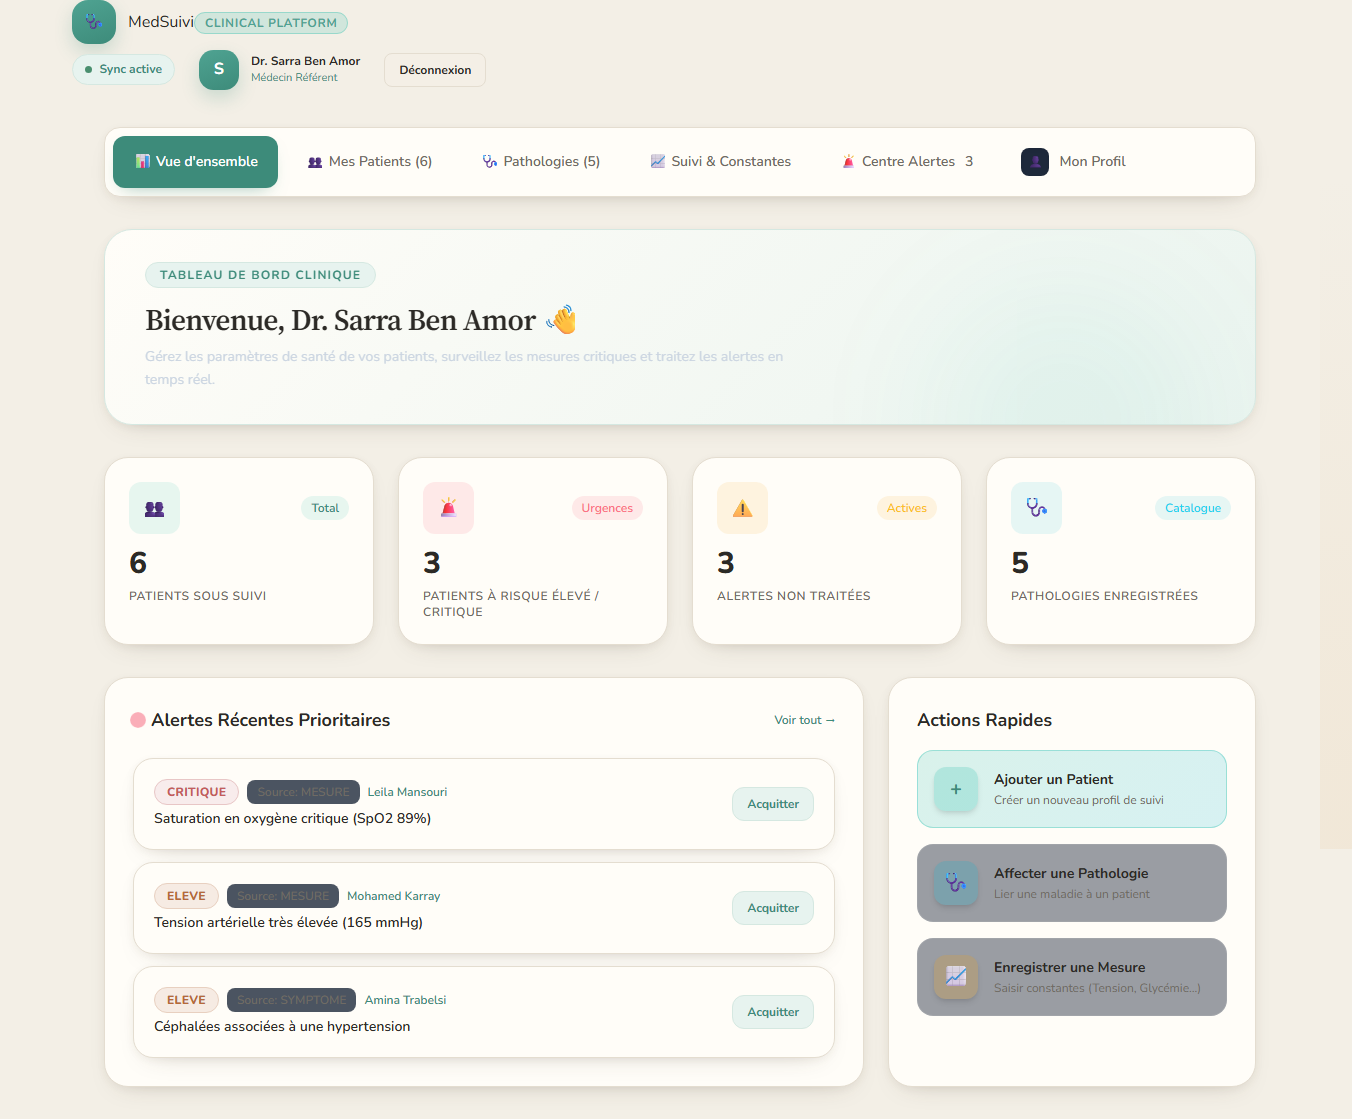
\includegraphics[width=0.85\textwidth]{rapport-screenshots/07-dashboard-overview.png}
  \caption{Interface tableau de bord (vue d'ensemble)}
  \label{fig:ui-overview}
\end{figure}

\section{CRUD patients et filtrage par niveau de risque}
L'onglet « Mes Patients » (figure~\ref{fig:ui-patients}) liste la patientèle
avec recherche et filtres par niveau de risque ; la création passe par un
formulaire modal (figure~\ref{fig:ui-add-patient}).

\begin{figure}[H]
  \centering
  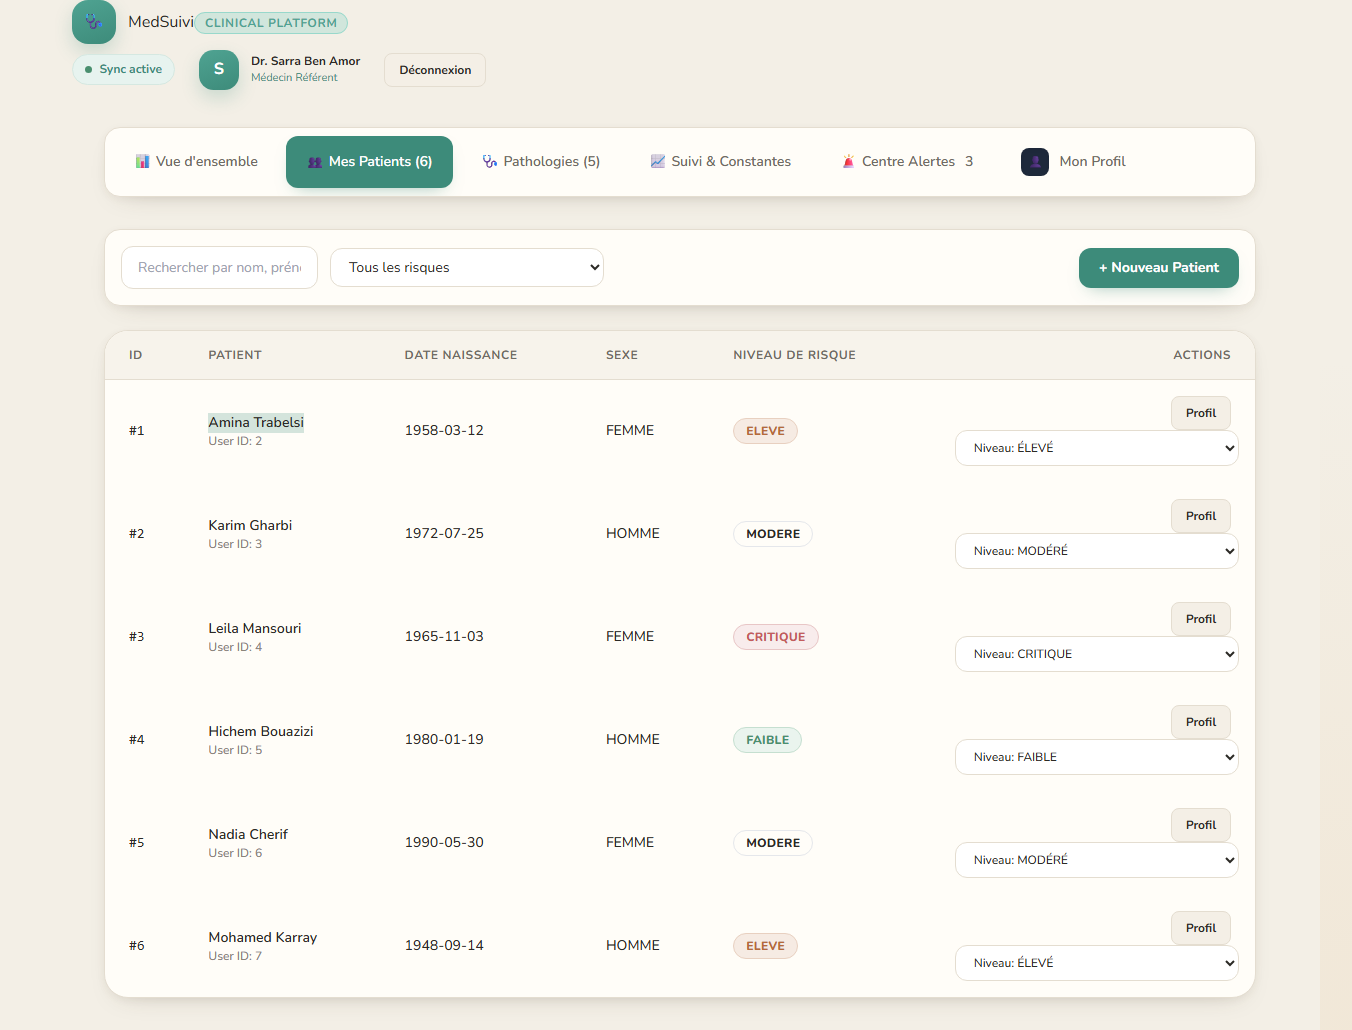
\includegraphics[width=0.85\textwidth]{rapport-screenshots/08-dashboard-patients.png}
  \caption{Interface « Mes patients »}
  \label{fig:ui-patients}
\end{figure}

\begin{figure}[H]
  \centering
  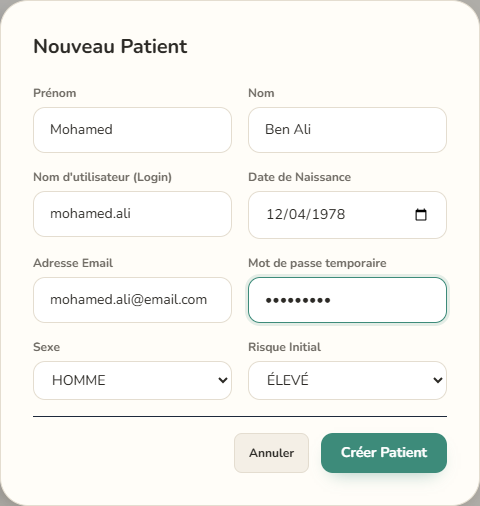
\includegraphics[width=0.5\textwidth]{rapport-screenshots/15-modal-add-patient.png}
  \caption{Interface « Création d'un patient »}
  \label{fig:ui-add-patient}
\end{figure}

\section{Gestion du catalogue de maladies}
L'onglet « Pathologies » (figure~\ref{fig:ui-maladies}) présente le catalogue
de maladies avec leurs paramètres suivis et leurs seuils cliniques.

\begin{figure}[H]
  \centering
  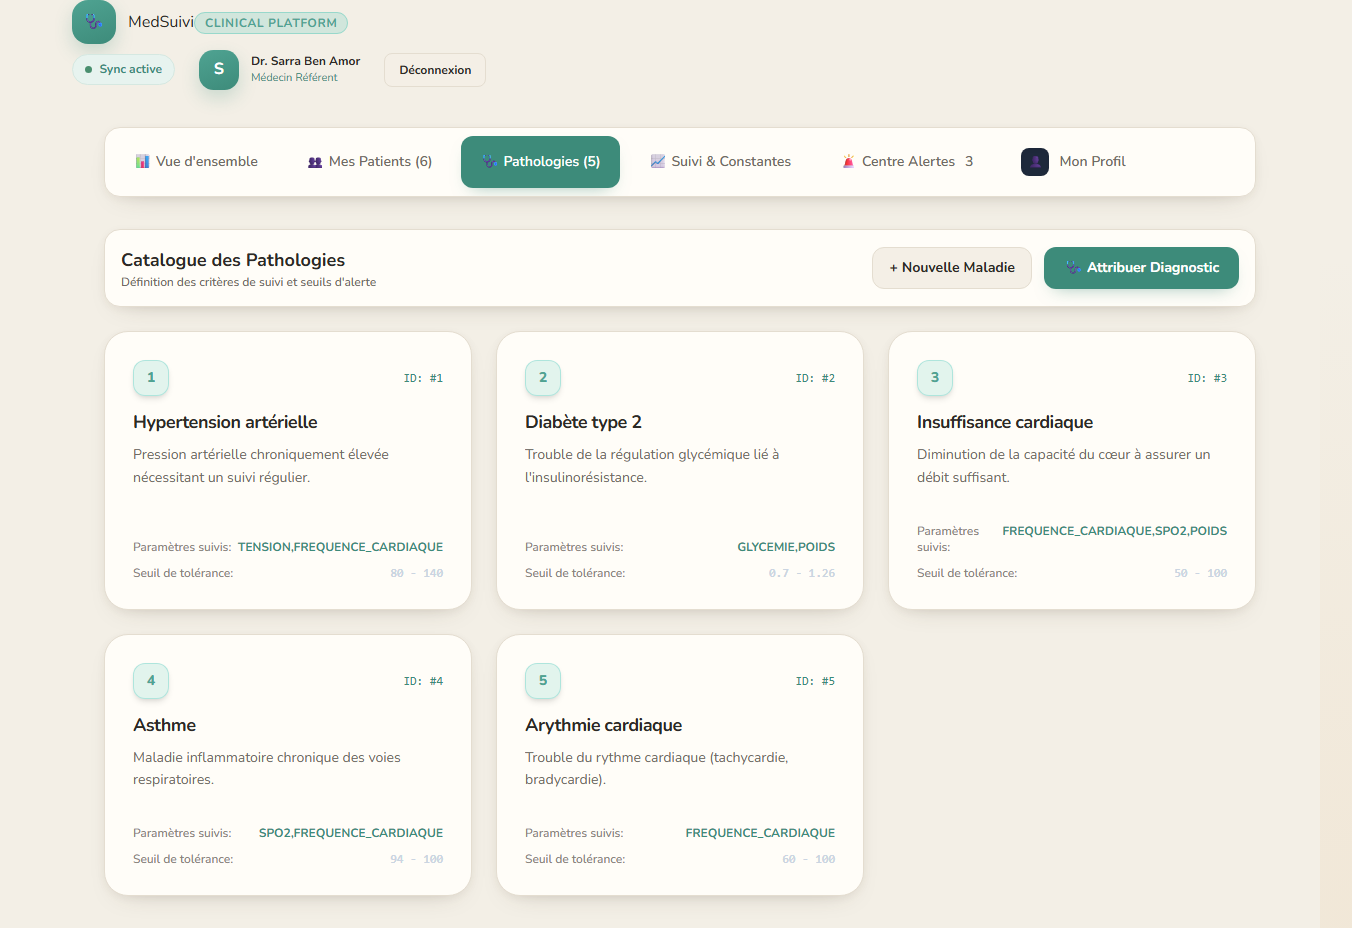
\includegraphics[width=0.85\textwidth]{rapport-screenshots/09-dashboard-pathologies.png}
  \caption{Interface « Pathologies »}
  \label{fig:ui-maladies}
\end{figure}

\section{Affectation d'une maladie à un patient}
L'affectation d'un diagnostic (figure~\ref{fig:ui-assign}) relie un patient à
une pathologie du catalogue en précisant la date du diagnostic.

\begin{figure}[H]
  \centering
  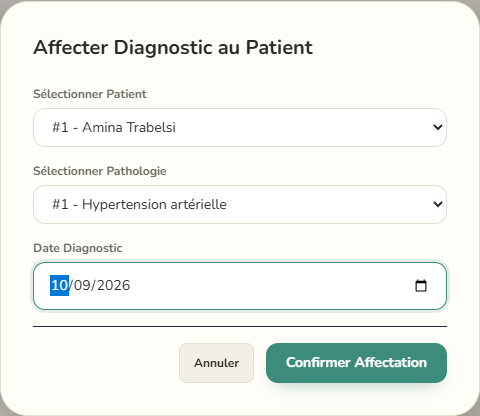
\includegraphics[width=0.5\textwidth]{rapport-screenshots/16-modal-assign-maladie.png}
  \caption{Interface « Affectation d'une maladie »}
  \label{fig:ui-assign}
\end{figure}

\section{Profil médecin (spécialité, numéro d'ordre)}
Le profil métier \texttt{Medecin} est lié au compte utilisateur (spécialité,
numéro d'ordre, liste de patients) ; il est créé automatiquement à la première
connexion du médecin.

% ============================================================
\chapter{Sprint 3 : Suivi médical (mesures et symptômes)}

Ce sprint couvre la collecte des données cliniques : saisie des constantes et
des symptômes par le médecin ou par le patient, puis restitution sous forme
d'historique et de courbe d'évolution.

\section{User stories du sprint}
\begin{itemize}[leftmargin=1.4em]
  \item En tant que médecin ou patient, je saisis une constante (tension, glycémie, \ldots).
  \item En tant que médecin, je consigne un symptôme et sa gravité.
  \item En tant que patient, je consulte l'historique et la courbe d'évolution.
\end{itemize}

\section{Diagramme de cas d'utilisation « Suivi médical »}
La figure~\ref{fig:uc-suivi} montre que la saisie des constantes est partagée
entre médecin et patient (auto-mesure), tandis que la consultation de la
courbe est incluse dans celle de l'historique.

\begin{figure}[H]
  \centering
  \begin{tikzpicture}[font=\small, >=Stealth]
    \draw[umlsys] (-1.1,-3.3) rectangle (4.9,3.1);
    \node[font=\small\bfseries] at (1.9,2.75) {Système MediSuivi --- \texttt{patient-service}};
    \umlactor{med}{-3.3,1.4}{Médecin}
    \umlactor{pat}{-3.3,-1.7}{Patient}
    \node[uc] (ucmes)   at (1.9,1.9)  {Saisir une constante};
    \node[uc] (ucsym)   at (1.9,0.6)  {Signaler un symptôme};
    \node[uc] (uchist)  at (1.9,-0.8) {Consulter l'historique};
    \node[uc] (uccourb) at (1.9,-2.2) {Courbe d'évolution};
    \draw (med) -- (ucmes.west);
    \draw (med) -- (ucsym.west);
    \draw (med) -- (uchist.west);
    \draw (pat) -- (ucmes.west);
    \draw (pat) -- (uchist.west);
    \draw (pat) -- (uccourb.west);
    \draw[->, dashed] (uchist.south) -- node[right, font=\scriptsize]{«include»} (uccourb.north);
  \end{tikzpicture}
  \caption{Diagramme de cas d'utilisation « Suivi médical »}
  \label{fig:uc-suivi}
\end{figure}

\section{Diagramme de séquence « saisie d'une mesure »}
La figure~\ref{fig:seq-mesure} décrit l'enregistrement d'une constante : le
service contrôle la valeur au regard des seuils de la pathologie avant de la
persister et de la restituer dans l'historique.

\begin{figure}[H]
  \centering
  \begin{tikzpicture}[font=\small, >=Stealth]
    \node[seqobj] (a)  at (0,0)    {Acteur};
    \node[seqobj] (ui) at (3.2,0)  {Interface};
    \node[seqobj] (gw) at (6.4,0)  {API Gateway};
    \node[seqobj] (ps) at (9.6,0)  {Patient Service};
    \node[seqobj] (db) at (12.6,0) {Base de données};
    \foreach \n in {a,ui,gw,ps,db} { \draw[dashed] (\n.south) -- ++(0,-6.4); }
    \draw[->] (0,-1.0) -- node[above, font=\scriptsize]{1. type, valeur, unité, source} (3.2,-1.0);
    \draw[->] (3.2,-1.8) -- node[above, font=\scriptsize]{2. POST /mesures} (6.4,-1.8);
    \draw[->] (6.4,-2.6) -- node[above, font=\scriptsize]{3. routage vers /patients/**} (9.6,-2.6);
    \draw[->] (9.6,-3.4) -- node[above, font=\scriptsize]{4. contrôle des seuils} (12.6,-3.4);
    \draw[->] (9.6,-4.2) -- node[above, font=\scriptsize]{5. INSERT mesure} (12.6,-4.2);
    \draw[->, dashed] (12.6,-5.0) -- node[above, font=\scriptsize]{6. 201 Created} (3.2,-5.0);
    \draw[->, dashed] (3.2,-5.8) -- node[above, font=\scriptsize]{7. historique actualisé} (0,-5.8);
  \end{tikzpicture}
  \caption{Diagramme de séquence « saisie d'une mesure »}
  \label{fig:seq-mesure}
\end{figure}

\section{Diagramme de classes du Sprint 3}
La figure~\ref{fig:class-s3} introduit les entités \texttt{Mesure} et
\texttt{Symptome}, toutes deux rattachées au patient qui en est la source.

\begin{figure}[H]
  \centering
  \begin{tikzpicture}[font=\small, >=Stealth]
    \begin{scope}[shift={(3.5,0)}]
      \umlclass{Patient}{Patient}{
        \texttt{id : Long} \\
        \texttt{nom / prenom : String} \\
        \texttt{niveauRisque : NiveauRisque}
      }{
        \texttt{+ getMesures()} \\
        \texttt{+ getSymptomes()}
      }
    \end{scope}
    \begin{scope}[shift={(0,-6)}]
      \umlclass{Mesure}{Mesure}{
        \texttt{id : Long} \\
        \texttt{patientId : Long} \\
        \texttt{typeMesure : TypeMesure} \\
        \texttt{valeur : Double} \\
        \texttt{unite : String} \\
        \texttt{source : Source} \\
        \texttt{dateMesure : DateTime}
      }{
        \texttt{+ depasseSeuil()}
      }
    \end{scope}
    \begin{scope}[shift={(7.5,-6)}]
      \umlclass{Symptome}{Symptome}{
        \texttt{id : Long} \\
        \texttt{patientId : Long} \\
        \texttt{description : String} \\
        \texttt{gravite : Gravite} \\
        \texttt{dateSymptome : DateTime}
      }{
        \texttt{+ estGrave()}
      }
    \end{scope}
    \draw[thick] (Patient.south) -- node[left, font=\scriptsize, pos=0.2]{1}
                             node[left, font=\scriptsize, pos=0.8]{0..*} (Mesure.north);
    \draw[thick] (Patient.south) -- node[right, font=\scriptsize, pos=0.2]{1}
                              node[right, font=\scriptsize, pos=0.8]{0..*} (Symptome.north);
  \end{tikzpicture}
  \caption{Diagramme de classes du Sprint 3}
  \label{fig:class-s3}
\end{figure}

\section{Saisie des constantes (tension, glycémie, etc.)}
Côté web, l'onglet « Suivi \& Constantes » (figure~\ref{fig:ui-suivi}) liste
les relevés et ouvre le formulaire de saisie
(figure~\ref{fig:ui-add-mesure}) ; côté mobile, l'écran « Saisie » propose le
même service au patient (figure~\ref{fig:ui-mesure-mobile}).

\begin{figure}[H]
  \centering
  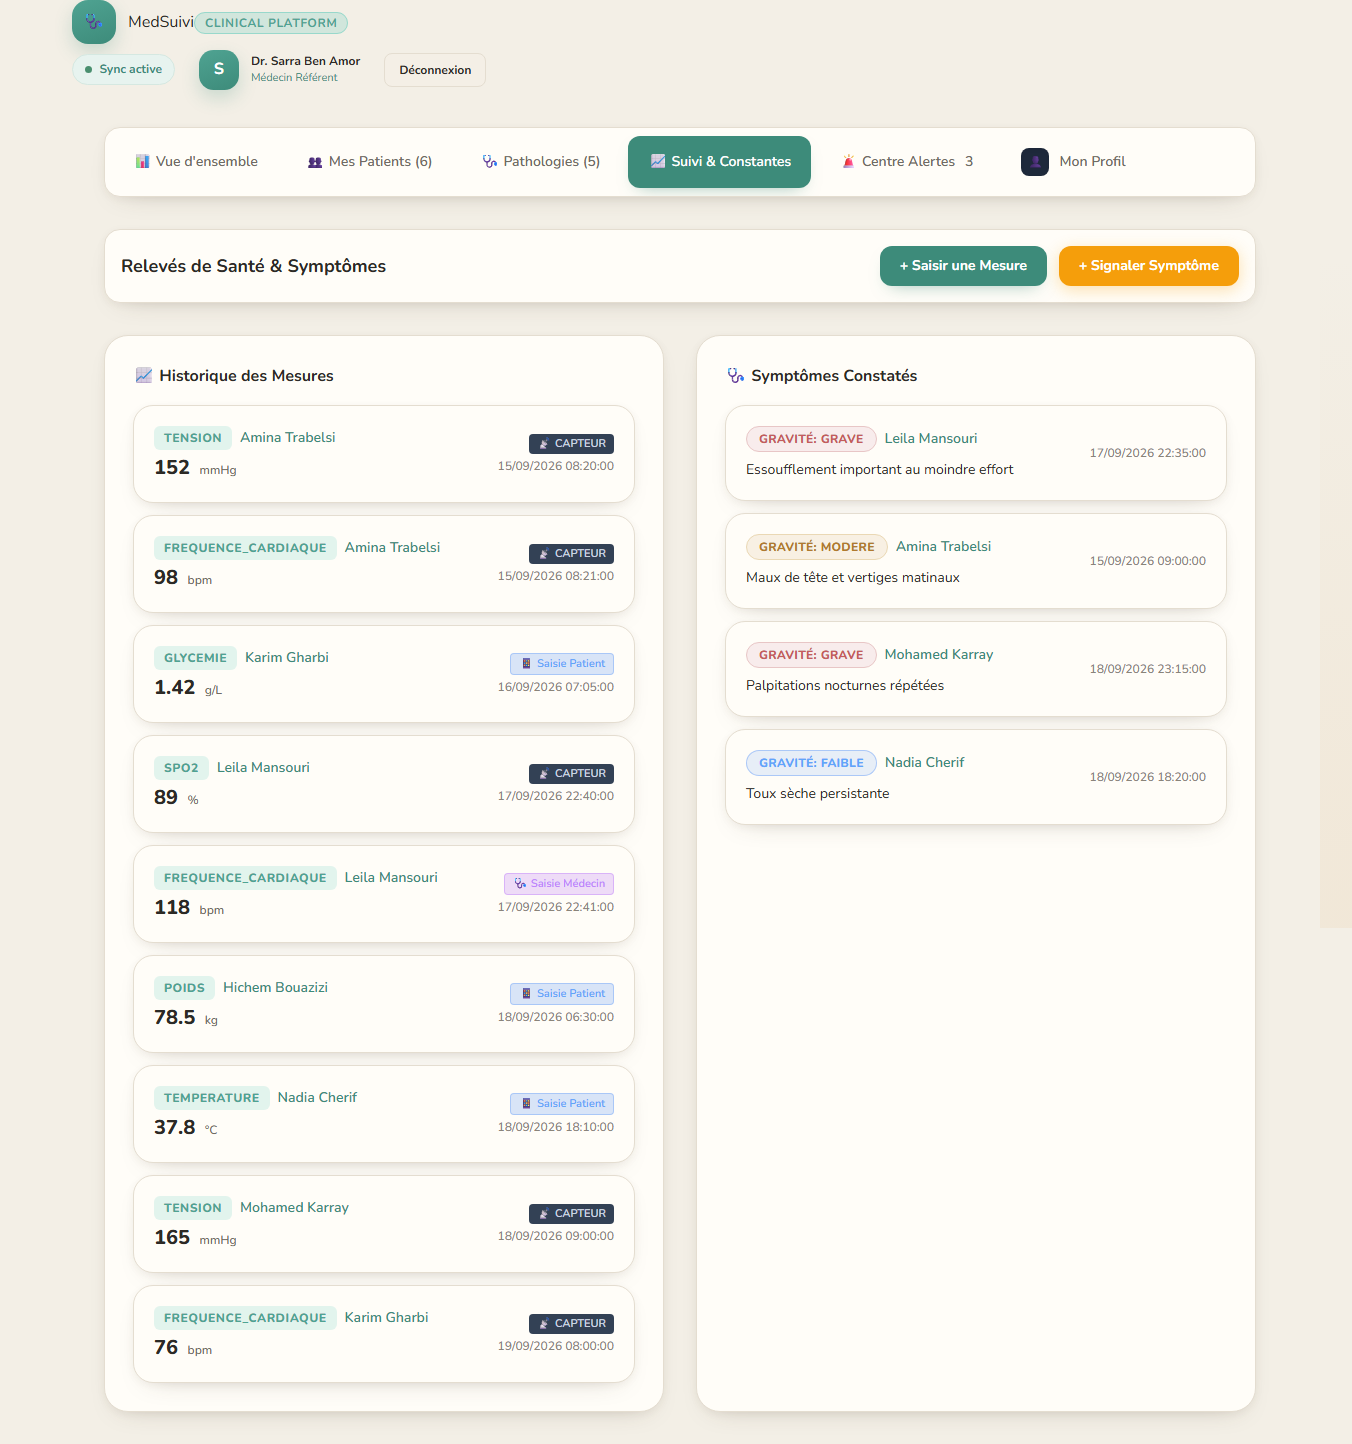
\includegraphics[width=0.85\textwidth]{rapport-screenshots/10-dashboard-suivi.png}
  \caption{Interface « Suivi \& Constantes » (web)}
  \label{fig:ui-suivi}
\end{figure}

\begin{figure}[H]
  \centering
  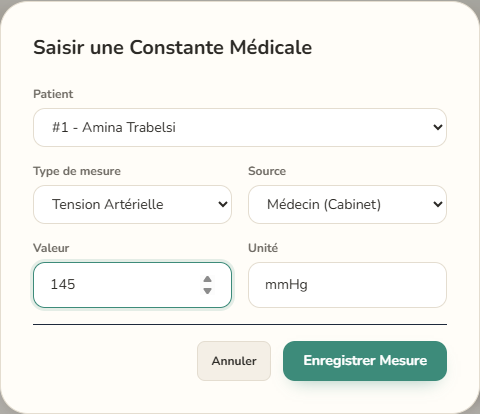
\includegraphics[width=0.5\textwidth]{rapport-screenshots/17-modal-add-mesure.png}
  \caption{Interface « Ajout d'une mesure » (web)}
  \label{fig:ui-add-mesure}
\end{figure}

\begin{figure}[H]
  \centering
  
\includegraphics[width=0.4\textwidth]{add_measure.png}
  \caption{Interface « Nouvelle mesure » (mobile)}
  \label{fig:ui-mesure-mobile}
\end{figure}

\section{Saisie des symptômes et gravité}
Le signalement d'un symptôme (figure~\ref{fig:ui-symptome}) précise une
description libre et un niveau de gravité (faible, modéré, grave).

\begin{figure}[H]
  \centering
  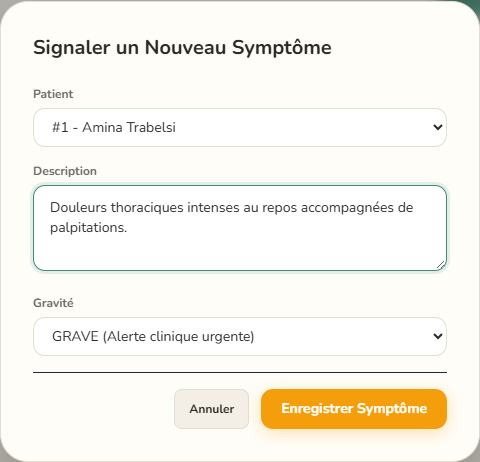
\includegraphics[width=0.5\textwidth]{rapport-screenshots/18-modal-add-symptome.png}
  \caption{Interface « Ajout d'un symptôme »}
  \label{fig:ui-symptome}
\end{figure}

\section{Historique des relevés (web et mobile)}
L'historique regroupe chronologiquement les mesures et symptômes d'un patient ;
la figure~\ref{fig:ui-historique} en donne la lecture côté mobile, avec
filtrage par période (7, 30 ou 90 jours).

\begin{figure}[H]
  \centering
  
\includegraphics[width=0.4\textwidth]{history.png}
  \caption{Interface « Historique des relevés »}
  \label{fig:ui-historique}
\end{figure}

\section{Courbe d'évolution des mesures}
Le mode « courbe » de l'écran historique (figure~\ref{fig:ui-courbe}) trace
l'évolution d'une constante sur la période choisie, ce qui permet de repérer
visuellement une dégradation.

\begin{figure}[H]
  \centering
  
\includegraphics[width=0.4\textwidth]{history.png}
  \caption{Courbe d'évolution des mesures}
  \label{fig:ui-courbe}
\end{figure}

% ============================================================
\chapter{Sprint 4 : Alertes médicales et urgence}

Ce sprint ferme la boucle de surveillance : toute situation à risque ---
alerte SOS du patient ou dépassement de seuil détecté automatiquement ---
remonte vers le médecin, qui la traite depuis son centre d'alertes.

\section{User stories du sprint}
\begin{itemize}[leftmargin=1.4em]
  \item En tant que patient, j'envoie une alerte SOS avec un niveau de risque.
  \item En tant que médecin, je consulte le centre d'alertes.
  \item En tant que médecin, je traite / clôture une alerte.
\end{itemize}

\section{Diagramme de cas d'utilisation « Gestion des alertes »}
La figure~\ref{fig:uc-alertes} distingue les alertes émises par le patient,
celles générées automatiquement par le système lors d'un dépassement de seuil,
et leur traitement par le médecin.

\begin{figure}[H]
  \centering
  \begin{tikzpicture}[font=\small, >=Stealth]
    \draw[umlsys] (-1.1,-3.3) rectangle (4.9,3.1);
    \node[font=\small\bfseries] at (1.9,2.75) {Système MediSuivi --- \texttt{patient-service}};
    \umlactor{pat}{-3.3,1.5}{Patient}
    \umlactor{sys}{-3.3,-1.0}{Système}
    \umlactor{med}{7.1,0}{Médecin}
    \node[uc] (ucsos)   at (1.9,1.9)  {Envoyer une alerte SOS};
    \node[uc] (ucauto)  at (1.9,0.5)  {Générer une alerte automatique};
    \node[uc] (uccons)  at (1.9,-0.9) {Consulter le centre d'alertes};
    \node[uc] (uctrait) at (1.9,-2.3) {Traiter / clôturer une alerte};
    \draw (pat) -- (ucsos.west);
    \draw (sys) -- (ucauto.west);
    \draw (med) -- (uccons.east);
    \draw (med) -- (uctrait.east);
    \draw[->, dashed] (uctrait.north) -- node[right, font=\scriptsize]{«include»} (uccons.south);
  \end{tikzpicture}
  \caption{Diagramme de cas d'utilisation « Gestion des alertes »}
  \label{fig:uc-alertes}
\end{figure}

\section{Diagramme de séquence « envoi d'une alerte SOS »}
La figure~\ref{fig:seq-alerte} suit une alerte SOS depuis l'application mobile
jusqu'à sa clôture par le médecin : l'alerte est créée non traitée, puis
acquittée via un appel dédié.

\begin{figure}[H]
  \centering
  \begin{tikzpicture}[font=\small, >=Stealth]
    \node[seqobj] (p)  at (0,0)    {Patient};
    \node[seqobj] (mo) at (3.2,0)  {App mobile};
    \node[seqobj] (gw) at (6.4,0)  {API Gateway};
    \node[seqobj] (ps) at (9.6,0)  {Patient Service};
    \node[seqobj] (md) at (12.8,0) {Médecin};
    \foreach \n in {p,mo,gw,ps,md} { \draw[dashed] (\n.south) -- ++(0,-7.0); }
    \draw[->] (0,-1.0) -- node[above, font=\scriptsize]{1. gravité + description} (3.2,-1.0);
    \draw[->] (3.2,-1.8) -- node[above, font=\scriptsize]{2. POST /alertes} (6.4,-1.8);
    \draw[->] (6.4,-2.6) -- node[above, font=\scriptsize]{3. routage vers /patients/**} (9.6,-2.6);
    \draw[->] (9.6,-3.4) -- ++(1.1,0) |- node[above right, font=\scriptsize]{4. INSERT alerte (traitee = false)} (9.6,-4.0);
    \draw[->, dashed] (9.6,-4.6) -- node[above, font=\scriptsize]{5. 201 Created} (3.2,-4.6);
    \draw[->, dashed] (3.2,-5.2) -- node[above, font=\scriptsize]{6. confirmation d'envoi} (0,-5.2);
    \draw[->] (12.8,-5.8) -- node[above, font=\scriptsize]{7. consultation du centre d'alertes} (9.6,-5.8);
    \draw[->] (12.8,-6.4) -- node[above, font=\scriptsize]{8. PATCH /alertes/\{id\}/traiter} (9.6,-6.4);
    \draw[->, dashed] (9.6,-6.9) -- node[above, font=\scriptsize]{9. alerte marquée traitée} (12.8,-6.9);
  \end{tikzpicture}
  \caption{Diagramme de séquence « alerte SOS »}
  \label{fig:seq-alerte}
\end{figure}

\section{Diagramme de classes du Sprint 4}
La figure~\ref{fig:class-s4} modélise l'entité \texttt{Alerte}, produite par un
patient et acquittée par un médecin.

\begin{figure}[H]
  \centering
  \begin{tikzpicture}[font=\small, >=Stealth]
    \begin{scope}[shift={(0,0)}]
      \umlclass{Patient}{Patient}{
        \texttt{id : Long} \\
        \texttt{nom / prenom : String}
      }{
        \texttt{+ sendAlerte()}
      }
    \end{scope}
    \begin{scope}[shift={(7,0)}]
      \umlclass{Alerte}{Alerte}{
        \texttt{id : Long} \\
        \texttt{patientId : Long} \\
        \texttt{niveauRisque : NiveauRisque} \\
        \texttt{source : Source} \\
        \texttt{description : String} \\
        \texttt{dateCreation : DateTime} \\
        \texttt{traitee : Boolean}
      }{
        \texttt{+ marquerTraitee()}
      }
    \end{scope}
    \begin{scope}[shift={(0,-6.5)}]
      \umlclass{Medecin}{Medecin}{
        \texttt{id : Long} \\
        \texttt{userId : Long}
      }{
        \texttt{+ getAlertes()} \\
        \texttt{+ traiterAlerte()}
      }
    \end{scope}
    \draw[thick] (Patient.east) -- node[above, font=\scriptsize, pos=0.15]{1}
                             node[above, font=\scriptsize, pos=0.85]{0..*} (Alerte.west);
    \draw[thick] (Medecin.east) -- node[left, font=\scriptsize, pos=0.2]{1}
                              node[left, font=\scriptsize, pos=0.8]{0..*} (Alerte.south);
  \end{tikzpicture}
  \caption{Diagramme de classes du Sprint 4}
  \label{fig:class-s4}
\end{figure}

\section{Envoi d'alerte depuis l'application patient}
L'écran « Alerte SOS » de l'application mobile
(figure~\ref{fig:ui-sos}) permet au patient de qualifier la gravité de son
alerte avant de l'envoyer au médecin associé à son dossier.

\begin{figure}[H]
  \centering
  
\includegraphics[width=0.4\textwidth]{alert.png}
  \caption{Interface « Alerte médicale \& urgence » (mobile)}
  \label{fig:ui-sos}
\end{figure}

\section{Centre d'alertes du médecin}
Le centre d'alertes (figure~\ref{fig:ui-alertes}) classe les alertes par
niveau de risque et indique leur source (mesure, symptôme ou génération
automatique) ainsi que leur état de traitement.

\begin{figure}[H]
  \centering
  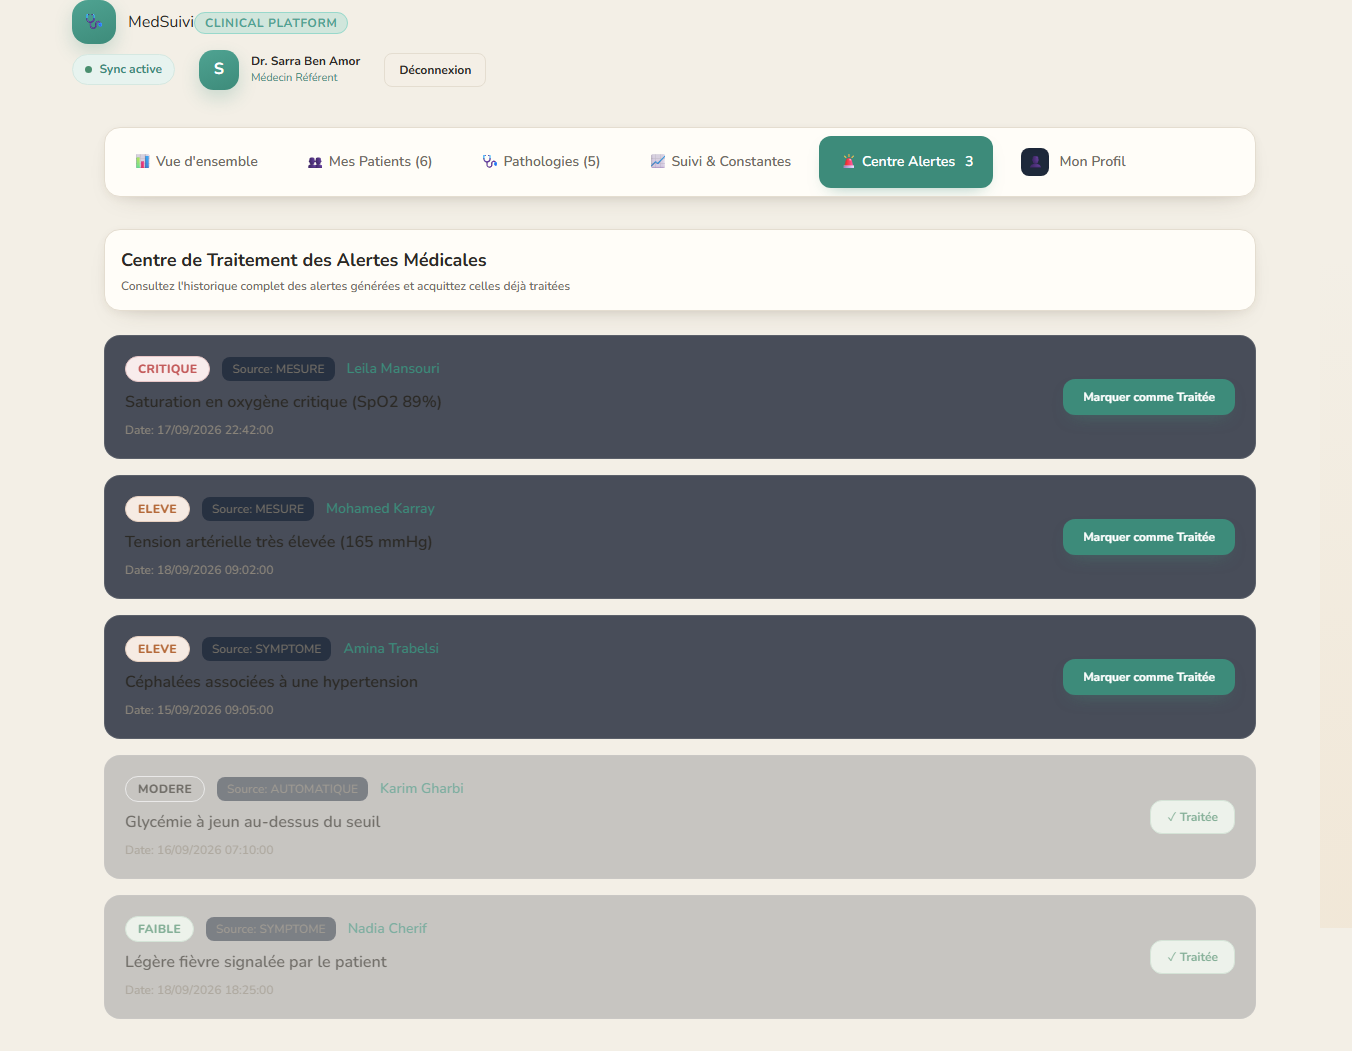
\includegraphics[width=0.85\textwidth]{rapport-screenshots/11-dashboard-alertes.png}
  \caption{Interface « Centre Alertes » (web)}
  \label{fig:ui-alertes}
\end{figure}

\section{Traitement / clôture d'une alerte}
Une fois prise en charge, l'alerte est acquittée par le médecin : la carte
passe à l'état « Traitée » et reste consultable dans l'historique
(figure~\ref{fig:ui-traiter}).

\begin{figure}[H]
  \centering
  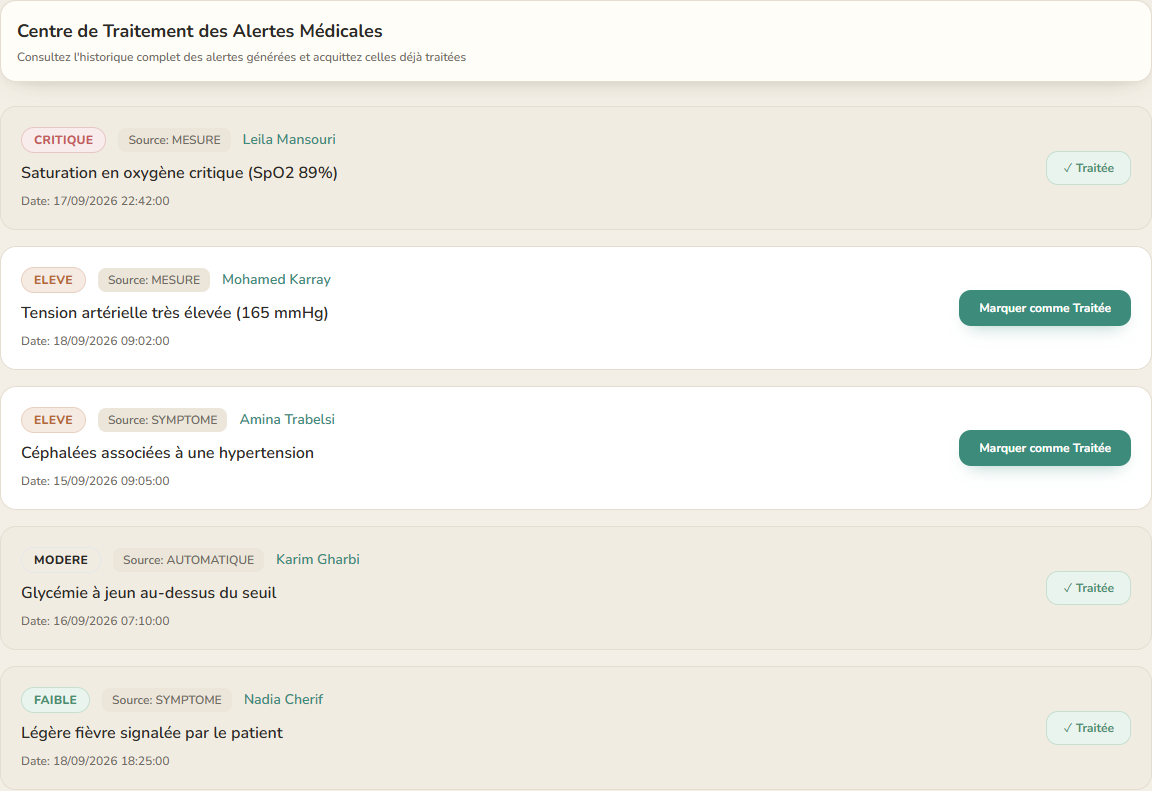
\includegraphics[width=0.85\textwidth]{rapport-screenshots/19-alertes-traitee.png}
  \caption{Interface « Traitement d'une alerte »}
  \label{fig:ui-traiter}
\end{figure}

\section{Appel d'urgence et contact du médecin traitant}
L'écran SOS mobile permet d'indiquer la gravité (faible à critique) et de
joindre le médecin associé au dossier.

% ============================================================
\chapter{Sprint 5 : Prédiction IA de la gravité}

\section{User stories du sprint}
\begin{itemize}[leftmargin=1.4em]
  \item En tant que médecin, je lance une prédiction de gravité pour un patient.
  \item En tant que système, je calcule des features (tendance 14~j, symptômes 7~j).
  \item En tant que médecin, je visualise les probabilités par classe de gravité.
\end{itemize}

\section{Diagramme de cas d'utilisation « Prédiction du risque »}
La figure~\ref{fig:uc-ia} cadre le périmètre du sprint : le médecin déclenche
la prédiction depuis la fiche patient ; le \texttt{patient-service} calcule les
features, interroge le service de prédiction puis met à jour le niveau de
risque. Si le service ML est injoignable, un cas d'extension applique une
évaluation par règles cliniques afin de ne jamais laisser la demande sans
réponse.

\begin{figure}[H]
  \centering
  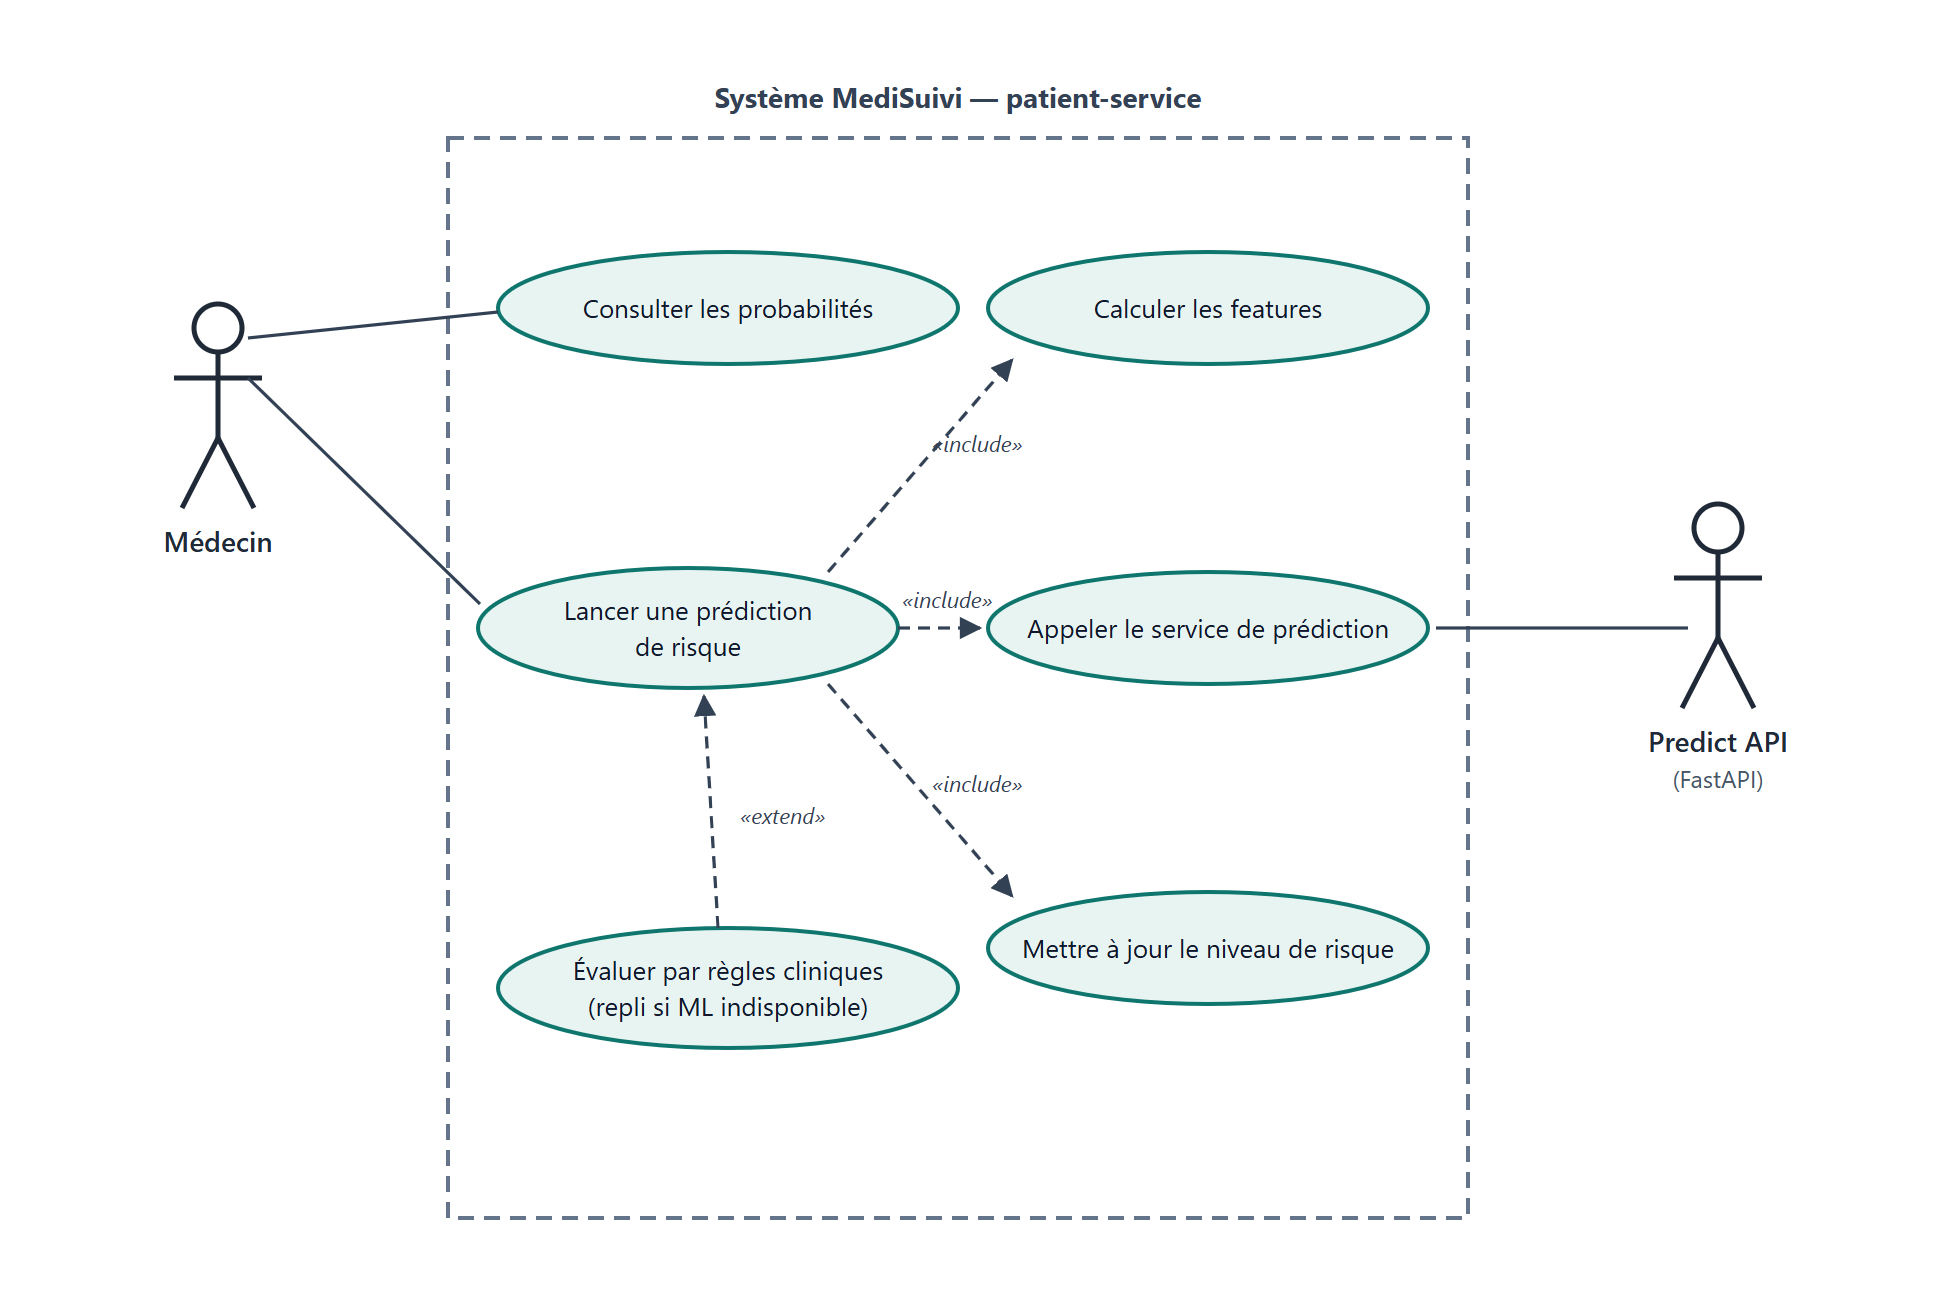
\includegraphics[width=0.95\textwidth]{rapport-screenshots/23-uc-ia.png}
  \caption{Diagramme de cas d'utilisation « Prédiction du risque »}
  \label{fig:uc-ia}
\end{figure}

\section{Pipeline de features (âge, maladie, tendance 14 j, symptômes 7 j)}
Le modèle ne reçoit pas les mesures brutes : le \texttt{patient-service} les
transforme d'abord en caractéristiques cliniques stables. La
figure~\ref{fig:features} détaille ce pipeline : les tables \texttt{Patient},
\texttt{PatientMaladie}, \texttt{Mesure} et \texttt{Symptome} alimentent
\texttt{buildRequestPayload()}, qui produit les dix variables attendues par le
modèle, dont la tendance glissante sur 14 jours (moyenne, écart-type, pente) et
le nombre de symptômes sur 7 jours.

\begin{figure}[H]
  \centering
  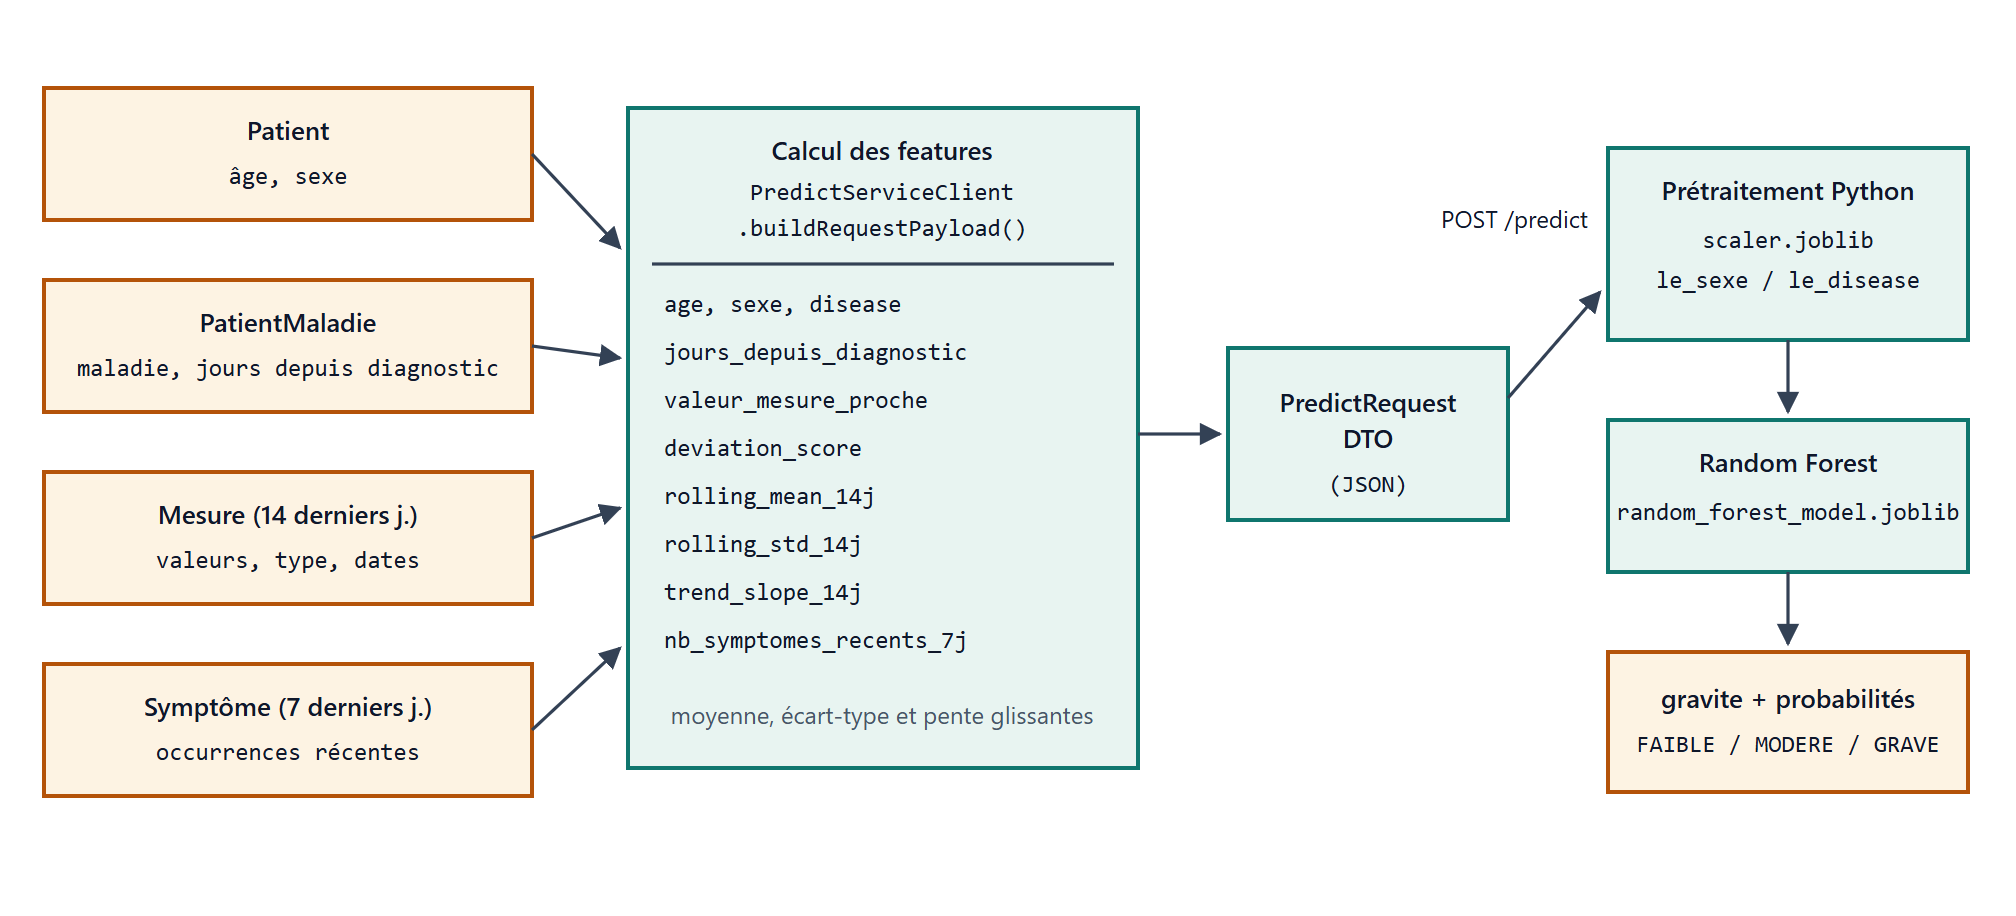
\includegraphics[width=0.98\textwidth]{rapport-screenshots/24-features-pipeline.png}
  \caption{Pipeline de features : des tables métier au vecteur d'entrée du modèle}
  \label{fig:features}
\end{figure}

Les variables exposées à l'API comprennent notamment : âge, sexe, maladie, jours depuis le diagnostic, valeur de mesure proche, score de déviation, moyenne / écart-type / pente sur 14 jours, nombre de symptômes récents sur 7 jours.

\section{Modèle Random Forest et API FastAPI}
La figure~\ref{fig:arch-rf} présente l'architecture logique du service Python.
L'endpoint \texttt{POST /predict} du service FastAPI valide la requête avec un
schéma Pydantic (\texttt{PatientFeatures}), normalise le sexe et la maladie
puis applique le scaler et les encodeurs sérialisés avant d'interroger le
modèle Random Forest (\texttt{random\_forest\_model.joblib}) chargé une seule
fois au démarrage. La réponse (\texttt{PredictionResponse}) contient la classe
de gravité prédite et les probabilités par classe ; l'endpoint
\texttt{GET /health} sert de sonde de vie pour le conteneur Docker.

\begin{figure}[H]
  \centering
  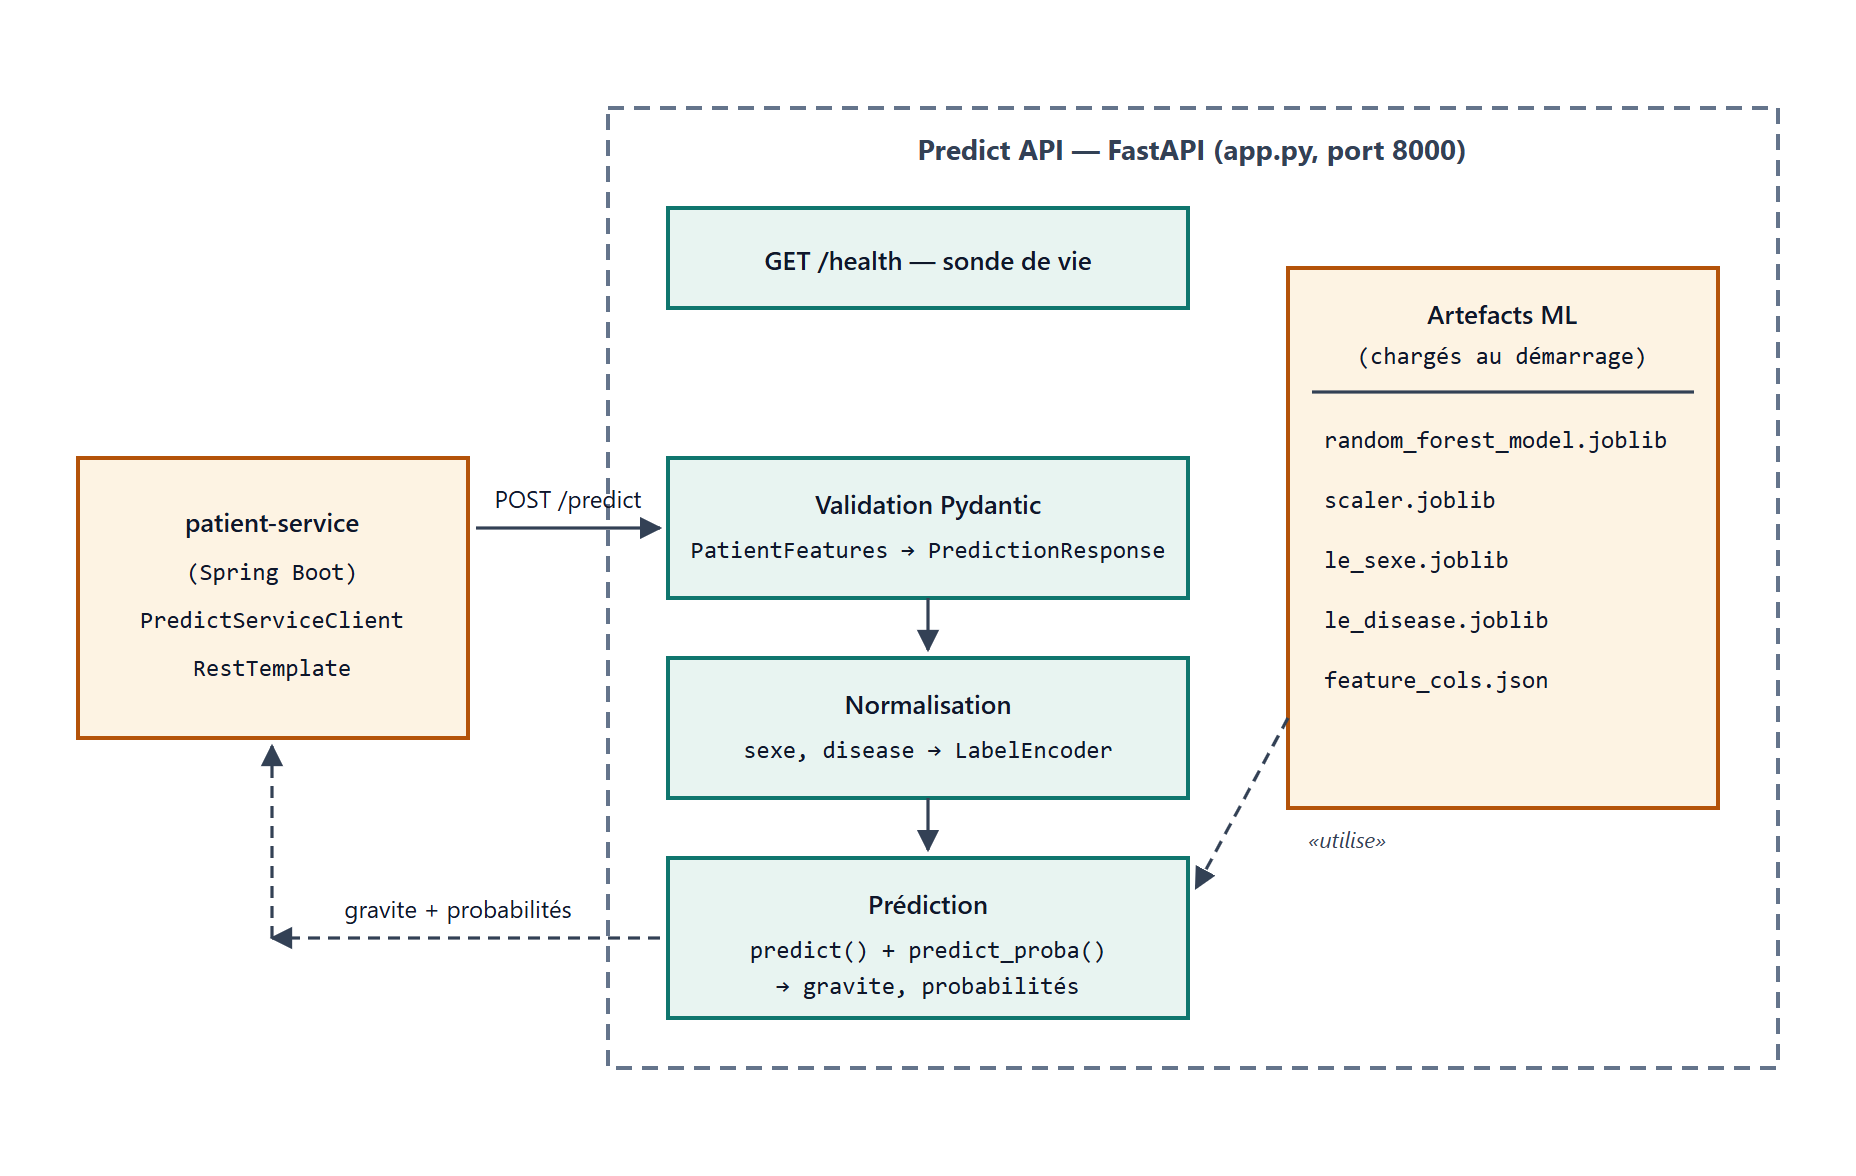
\includegraphics[width=0.95\textwidth]{rapport-screenshots/25-arch-predict-api.png}
  \caption{Architecture logique de la Predict API (FastAPI)}
  \label{fig:arch-rf}
\end{figure}

\section{Intégration Patient Service → Predict API}
Le \texttt{patient-service} appelle l'API Python via
\texttt{PredictServiceClient} (route \texttt{/patients/\{id\}/predict-risk}).
La figure~\ref{fig:class-s5} donne la structure des classes côté Java : le
contrôleur délègue au client, qui construit le \texttt{PredictRequestDTO},
consomme le \texttt{PredictResponseDTO} et reporte la gravité obtenue sur le
niveau de risque du patient ; en cas d'indisponibilité du service ML,
\texttt{evaluateRuleBasedRisk()} applique le repli clinique décrit plus haut.

\begin{figure}[H]
  \centering
  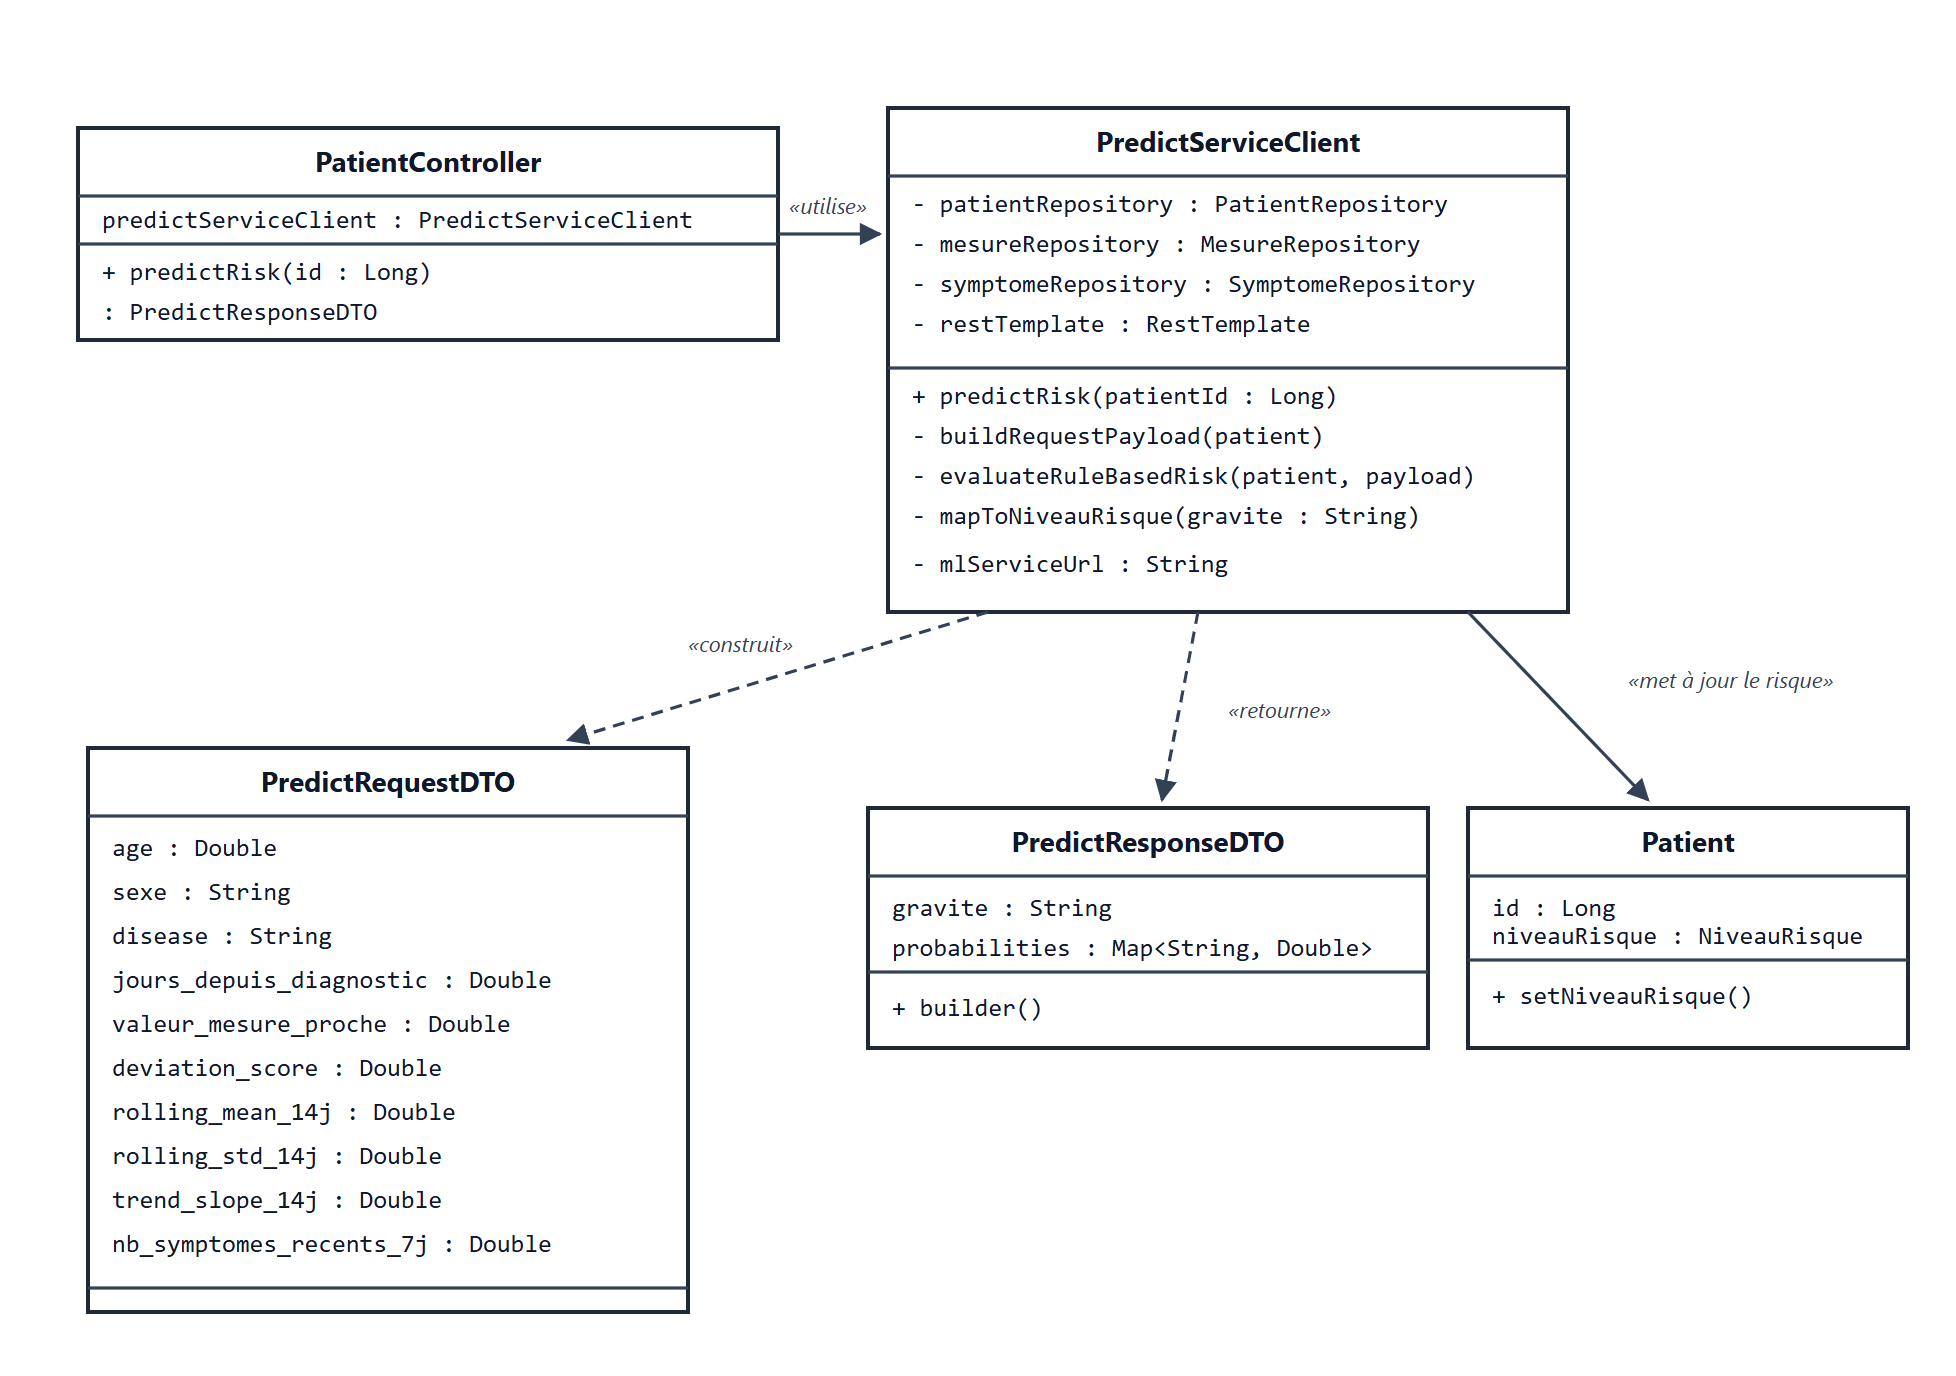
\includegraphics[width=0.95\textwidth]{rapport-screenshots/26-class-s5.png}
  \caption{Diagramme de classes du Sprint 5}
  \label{fig:class-s5}
\end{figure}

\section{Interface de scoring / prédiction côté médecin}
Depuis la fiche patient (figure~\ref{fig:ui-predict}), le médecin lance la
prédiction : le portail affiche alors la classe de gravité retenue ainsi que
les probabilités par classe renvoyées par le modèle
(figure~\ref{fig:ui-scoring}), ce qui permet de justifier la décision auprès du
patient.

\begin{figure}[H]
  \centering
  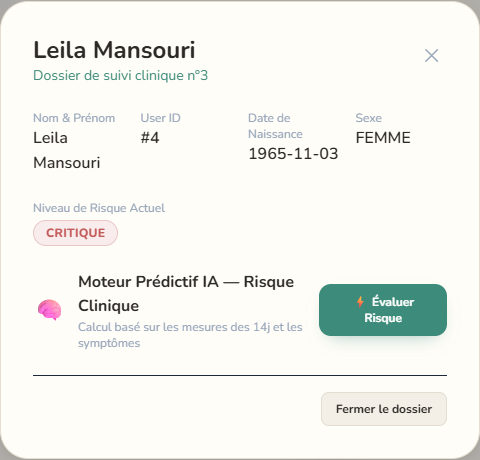
\includegraphics[width=0.85\textwidth]{rapport-screenshots/13-patient-fiche-predict.png}
  \caption{Fiche patient — lancement de la prédiction de gravité}
  \label{fig:ui-predict}
\end{figure}

\begin{figure}[H]
  \centering
  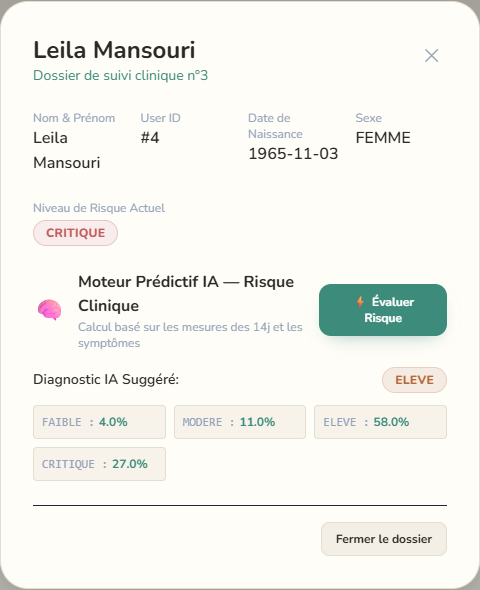
\includegraphics[width=0.85\textwidth]{rapport-screenshots/14-predict-result.png}
  \caption{Résultat du scoring : gravité prédite et probabilités par classe}
  \label{fig:ui-scoring}
\end{figure}

\section{Mise à jour du niveau de risque patient}
La gravité prédite (\texttt{FAIBLE}, \texttt{MODERE}, \texttt{GRAVE}) est
convertie en \texttt{NiveauRisque} puis persistée sur le patient : la liste des
patients (figure~\ref{fig:ui-badge}) reflète immédiatement le nouveau niveau,
ce qui permet au médecin de filtrer et de prioriser sa file active.

\begin{figure}[H]
  \centering
  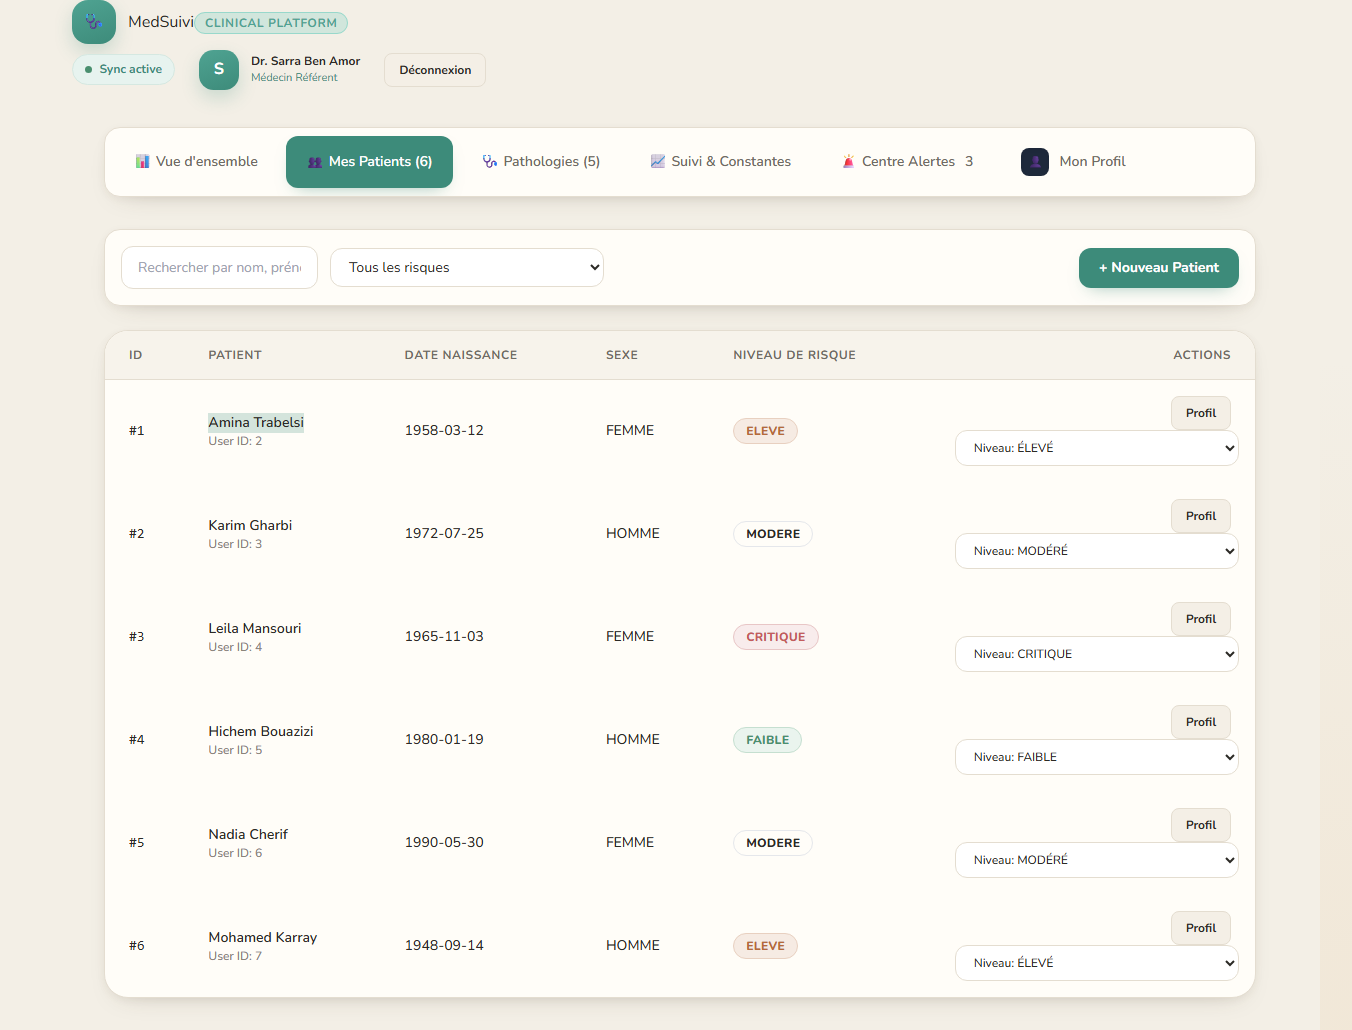
\includegraphics[width=0.85\textwidth]{rapport-screenshots/08-dashboard-patients.png}
  \caption{Badge de niveau de risque sur la liste des patients}
  \label{fig:ui-badge}
\end{figure}

% ============================================================
\chapter{Application mobile patient}

\section{Architecture de l'application Expo / React Native}
Navigation par pile (auth / espace connecté) et onglets : Accueil, Saisie, Alerte SOS, Historique, Profil.

\figplaceholder{fig:nav-mobile}{Navigation par onglets de l'application patient}

\section{Authentification patient}
Connexion au \texttt{user-service} via la Gateway, conservation de la session et chargement du profil patient.

\section{Tableau de bord patient et badge de risque}
\figplaceholder{fig:ui-dash-mobile}{Interface tableau de bord patient}

\section{Nouvelle mesure}
Saisie d'un type de constante et d'une valeur, envoi au \texttt{patient-service}.

\section{Alerte SOS}
Création d'une alerte non traitée, visible ensuite dans le centre d'alertes du médecin.

\section{Historique des relevés}
Liste chronologique des mesures du patient.

\section{Profil patient}
\figplaceholder{fig:ui-profil-mobile}{Interface profil patient}

% ============================================================
\chapter{Tests, qualité et DevOps}

\section{Tests unitaires et d'intégration (backend)}
Tests JUnit des contrôleurs, services et dépôts (\texttt{user-service}, \texttt{patient-service}).

\section{Tests frontend (Vitest) et couverture Jacoco / pytest}
\figplaceholder{fig:jacoco}{Couverture des tests (Jacoco)}

\section{Analyse SonarQube}
\figplaceholder{fig:sonar}{Interface SonarQube}

\section{Pipeline Jenkins backend}
Checkout, compilation Maven multi-modules, tests, Sonar, package, build \& push Docker (gateway, discovery, config-server, user-service, patient-service).

\figplaceholder{fig:jenkins-back}{Pipeline Jenkins backend}

\section{Pipeline Jenkins Predict API}
Installation des dépendances, build Docker, pytest + coverage, Sonar, push Docker Hub.

\figplaceholder{fig:jenkins-ml}{Pipeline Jenkins Predict API}

\section{Docker et Docker Hub}
Images des microservices et de l'API de prédiction publiées pour le déploiement.

\section{Architecture DevOps}
\begin{figure}[H]
  \centering
  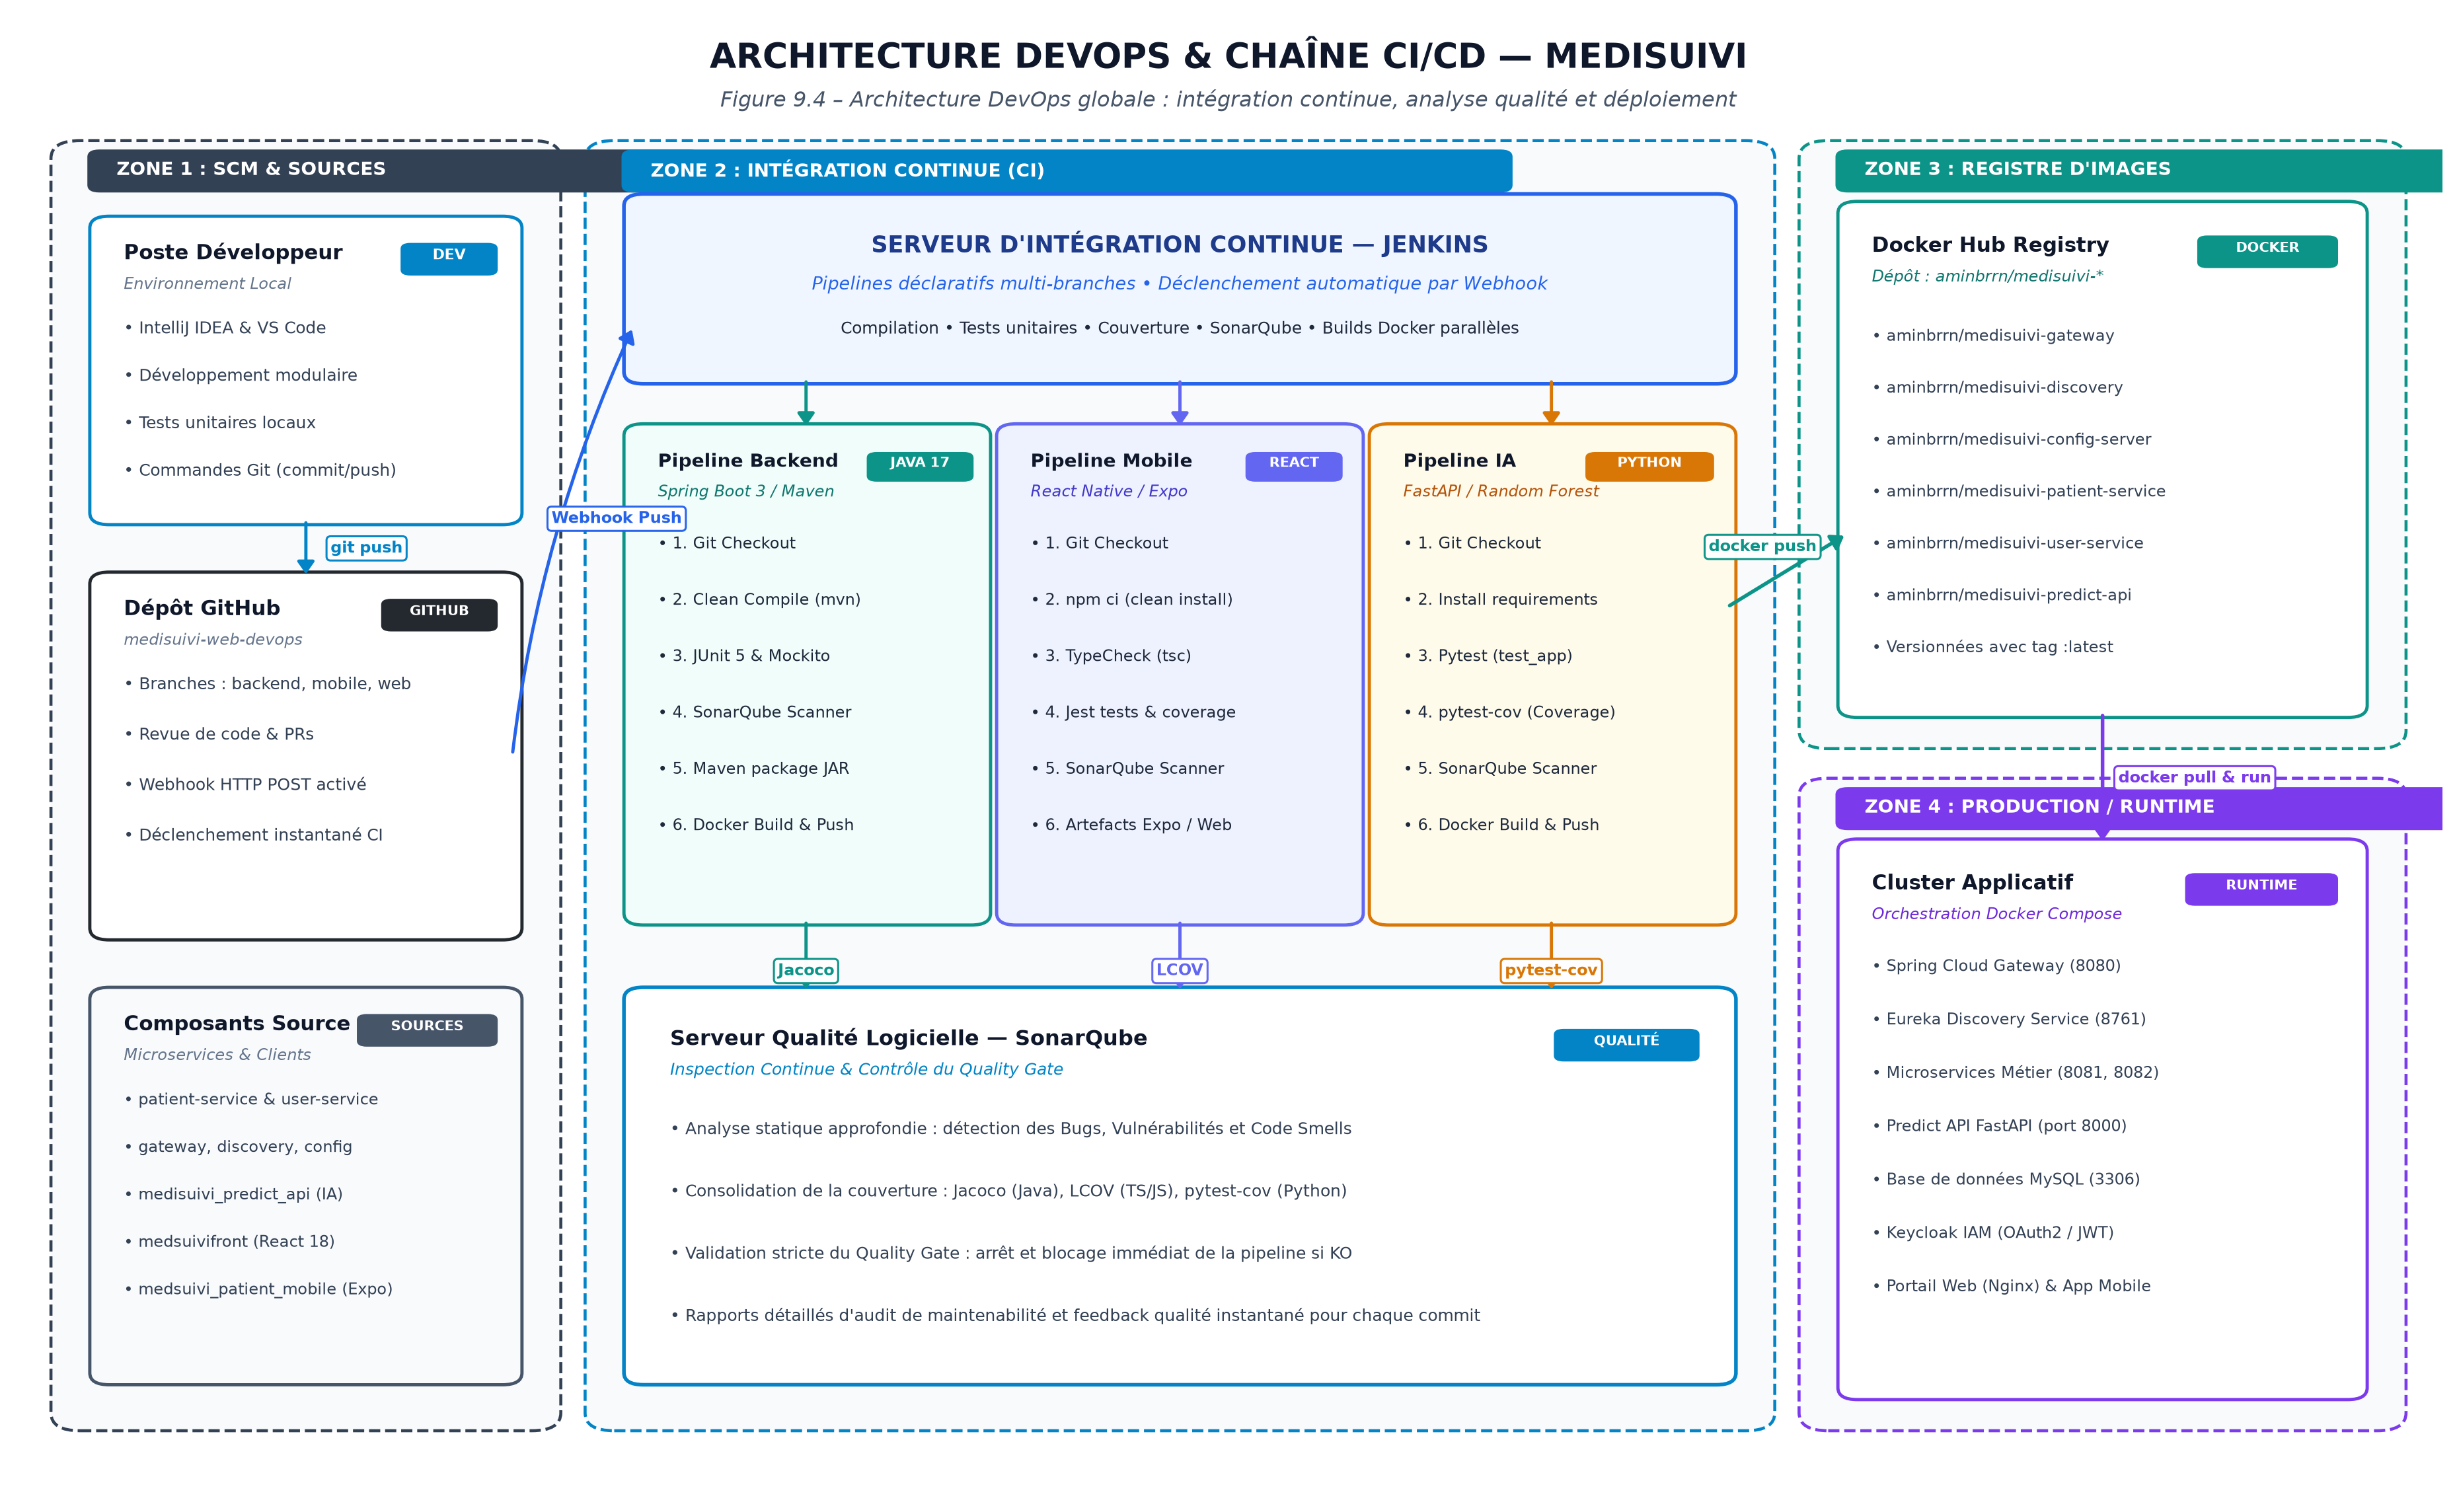
\includegraphics[width=0.98\textwidth]{rapport-screenshots/27-arch-devops.png}
  \caption{Architecture DevOps}
  \label{fig:arch-devops}
\end{figure}

\begin{figure}[H]
  \centering
  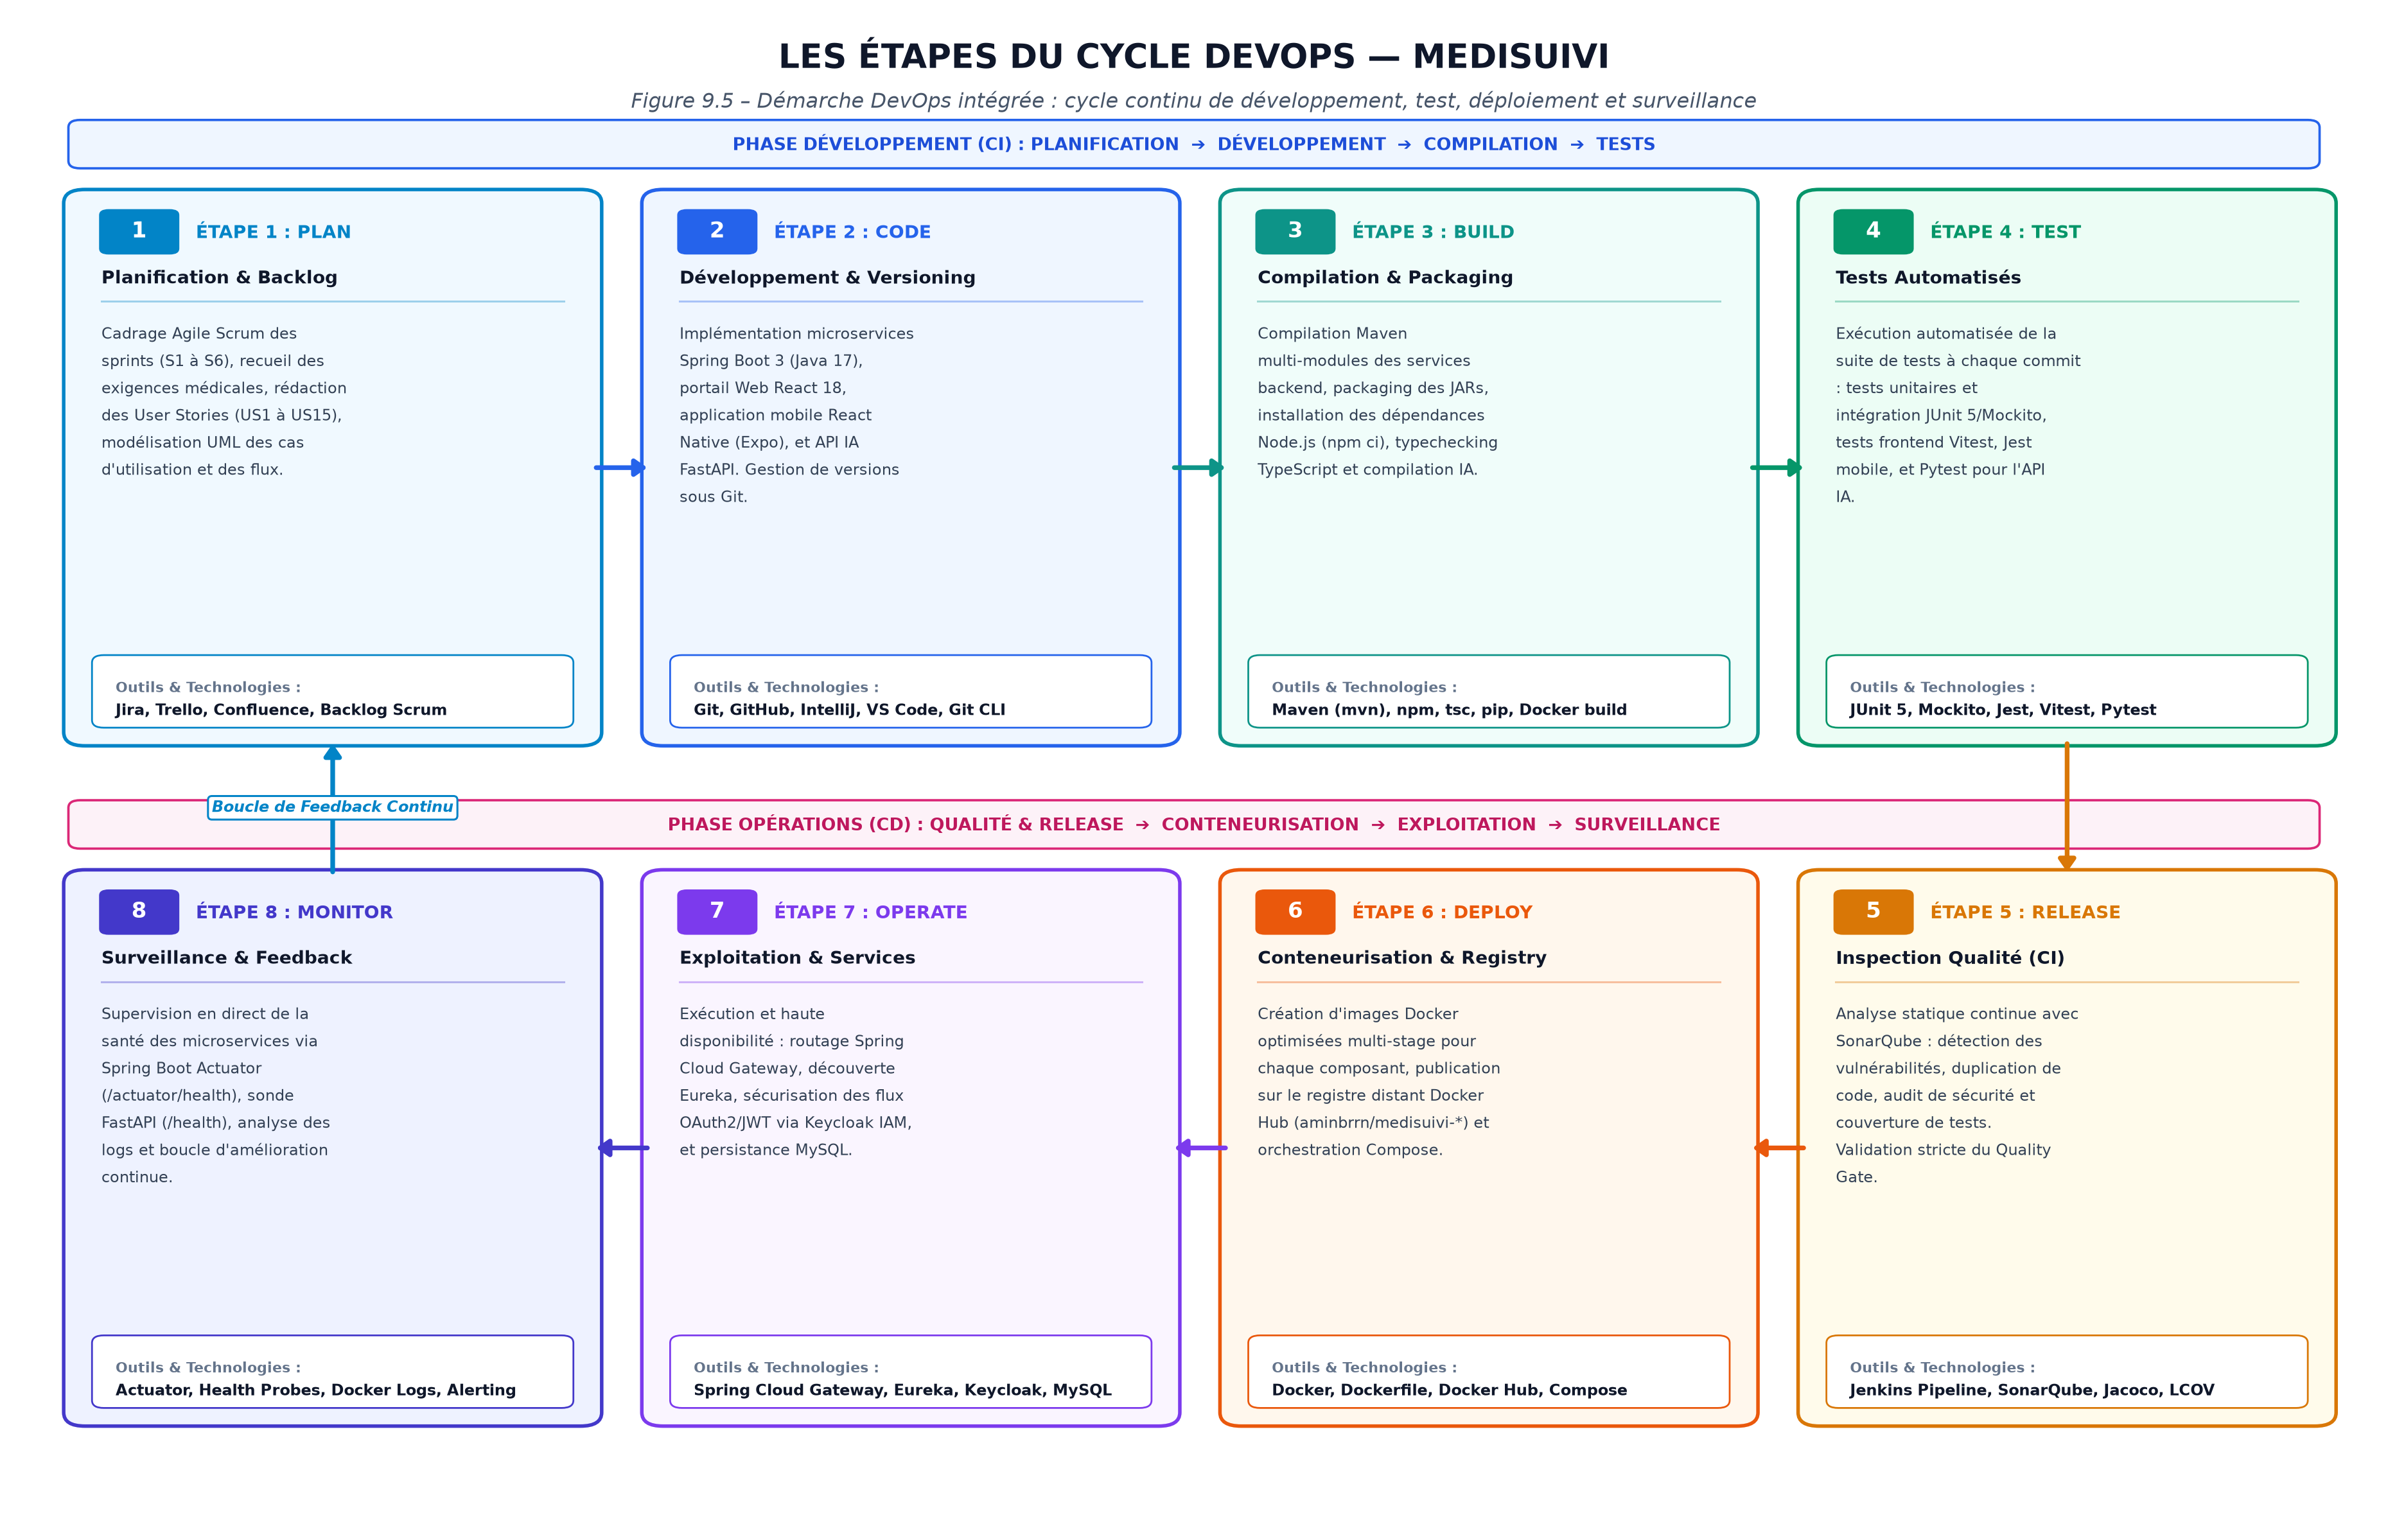
\includegraphics[width=0.98\textwidth]{rapport-screenshots/28-etapes-devops.png}
  \caption{Les étapes du DevOps}
  \label{fig:etapes-devops}
\end{figure}

% ============================================================
\chapter*{Conclusion et perspectives}
\addcontentsline{toc}{chapter}{Conclusion et perspectives}

MediSuivi relie un portail médecin, une application patient, une architecture microservices et un service de prédiction de gravité. Les perspectives incluent les notifications push temps réel, un suivi multi-pathologies plus fin, et le déploiement Kubernetes.

\chapter*{Bibliographie}
\addcontentsline{toc}{chapter}{Bibliographie}
\begin{itemize}[leftmargin=1.4em]
  \item Documentation Spring Cloud, React, React Native / Expo, FastAPI, scikit-learn.
  \item \textit{À compléter avec les ouvrages et normes réellement cités.}
\end{itemize}

\chapter*{Webographie}
\addcontentsline{toc}{chapter}{Webographie}
\begin{itemize}[leftmargin=1.4em]
  \item \url{https://spring.io/projects/spring-cloud}
  \item \url{https://react.dev}
  \item \url{https://docs.expo.dev}
  \item \url{https://fastapi.tiangolo.com}
\end{itemize}

\chapter*{Annexes}
\addcontentsline{toc}{chapter}{Annexes}
Annexe A : extraits d'API. Annexe B : user stories détaillées. Annexe C : captures d'écran supplémentaires.

\end{document}
